\documentclass[11pt,letterpaper]{article}

\usepackage[margin=0.9in]{geometry}
\usepackage{amsmath,amssymb}
\usepackage{graphicx}
\usepackage{booktabs}
\usepackage{enumitem}
\usepackage{float}
\usepackage{caption}
\usepackage[colorlinks=true,linkcolor=blue,citecolor=blue,urlcolor=blue]{hyperref}

\setlist{itemsep=2pt,topsep=3pt}
\captionsetup{font=small}
\graphicspath{{../results/figures/}}

\newcommand{\EoneNLLERfifty}{0.242}
\newcommand{\EoneNLMean}{0.144}
\newcommand{\EoneNLTrials}{60{,}000}
\newcommand{\EoneNLEvents}{14542}
\newcommand{\EoneBayesLERfifty}{8.5\!\times\!10^{-4}}
\newcommand{\EoneBayesMean}{1.5\!\times\!10^{-3}}
\newcommand{\EoneBayesTrials}{60{,}000}
\newcommand{\EoneBayesEvents}{51}
\newcommand{\EoneBayesPRLERfifty}{0.012}
\newcommand{\EoneBayesPRMean}{0.011}
\newcommand{\EoneBayesPRTrials}{60{,}000}
\newcommand{\EoneBayesPREvents}{718}
\newcommand{\EoneBayesBroadLERfifty}{9.7\!\times\!10^{-4}}
\newcommand{\EoneBayesBroadMean}{1.9\!\times\!10^{-3}}
\newcommand{\EoneBayesBroadTrials}{60{,}000}
\newcommand{\EoneBayesBroadEvents}{58}
\newcommand{\EoneLSTMnomLERfifty}{6.6\!\times\!10^{-3}}
\newcommand{\EoneLSTMnomMean}{5.5\!\times\!10^{-3}}
\newcommand{\EoneLSTMnomTrials}{60{,}000}
\newcommand{\EoneLSTMnomEvents}{1196}
\newcommand{\EoneLSTMbroadLERfifty}{0.015}
\newcommand{\EoneLSTMbroadMean}{0.010}
\newcommand{\EoneLSTMbroadTrials}{60{,}000}
\newcommand{\EoneLSTMbroadEvents}{2691}
\newcommand{\EoneLSTMkzeroLERfifty}{0.020}
\newcommand{\EoneLSTMkzeroMean}{0.017}
\newcommand{\EoneLSTMkzeroTrials}{60{,}000}
\newcommand{\EoneLSTMkzeroEvents}{1211}
\newcommand{\EoneNoneLERfifty}{0.501}
\newcommand{\EoneNoneMean}{0.481}
\newcommand{\EoneNoneTrials}{60{,}000}
\newcommand{\EoneNoneEvents}{30061}
\newcommand{\EoneGain}{95}
\newcommand{\EoneLSTMoverBayes}{3.7}
\newcommand{\EfiveSmHalfMean}{2.0\!\times\!10^{-3}}
\newcommand{\EfiveSmTwoMean}{3.0\!\times\!10^{-3}}
\newcommand{\EfiveNLMean}{0.141}
\newcommand{\EfiveLSTMnomMean}{5.3\!\times\!10^{-3}}
\newcommand{\EfiveLSTMbroadMean}{0.010}
\newcommand{\EfiveBayesMean}{1.5\!\times\!10^{-3}}
\newcommand{\EfiveRhoZeroMean}{0.195}
\newcommand{\EfiveRhoHalfMean}{7.8\!\times\!10^{-3}}
\newcommand{\EfiveRhoHighMean}{0.014}
\newcommand{\EfiveSqTwoMean}{2.2\!\times\!10^{-3}}
\newcommand{\EfiveSqHalfMean}{4.5\!\times\!10^{-3}}
\newcommand{\EfiveTrials}{40{,}000}
\newcommand{\EsixNLMean}{0.195}
\newcommand{\EsixBayesregimeawareMean}{0.130}
\newcommand{\EsixBayesrhozeronineMean}{0.162}
\newcommand{\EsixBayesrhozeroninesevenMean}{0.191}
\newcommand{\EsixBayesbroadMean}{0.147}
\newcommand{\EsixLSTMnominalMean}{0.176}
\newcommand{\EsixLSTMbroadMean}{0.142}
\newcommand{\EsixLSTMswitchingMean}{0.143}
\newcommand{\GPUname}{NVIDIA GeForce RTX 5080 Laptop GPU}
\newcommand{\ErevBayes}{1.5\!\times\!10^{-3}}
\newcommand{\ErevBayesPR}{0.011}
\newcommand{\ErevLSTM}{6.3\!\times\!10^{-3}}
\newcommand{\ErevLSTMkzero}{0.017}
\newcommand{\EhzNLFifty}{0.240}
\newcommand{\EhzNLTwohundred}{0.463}
\newcommand{\EhzBayesFifty}{9.5\!\times\!10^{-4}}
\newcommand{\EhzBayesTwohundred}{2.6\!\times\!10^{-3}}
\newcommand{\EhzLSTMnomFifty}{6.8\!\times\!10^{-3}}
\newcommand{\EhzLSTMnomTwohundred}{0.018}
\newcommand{\EhzLSTMbroadFifty}{6.0\!\times\!10^{-3}}
\newcommand{\EhzLSTMbroadTwohundred}{0.016}
\newcommand{\EpairZero}{0.05}
\newcommand{\EcancelZero}{0.04}
\newcommand{\EpairNominal}{0.48}
\newcommand{\EcancelNominal}{0.29}
\newcommand{\EpairHigh}{0.55}
\newcommand{\EcancelHigh}{0.31}
\newcommand{\EdiagDisagree}{5.9\!\times\!10^{-3}}
\newcommand{\EdiagBayesRight}{98}
\makeatletter
\newcommand{\res}[3]{\@ifundefined{res@#1@#2@#3}{??}{\csname res@#1@#2@#3\endcsname}}
\newcommand{\resfifty}[3]{\@ifundefined{rfifty@#1@#2@#3}{??}{\csname rfifty@#1@#2@#3\endcsname}}
\newcommand{\resratio}[3]{\@ifundefined{rratio@#1@#2@#3}{??}{\csname rratio@#1@#2@#3\endcsname}}
\newcommand{\tim}[4]{\@ifundefined{tim@#1@#2@#3@#4}{??}{\csname tim@#1@#2@#3@#4\endcsname}}
\makeatother
\expandafter\def\csname res@E1@nominal@Bayes-broad\endcsname{1.9\!\times\!10^{-3}}
\expandafter\def\csname rfifty@E1@nominal@Bayes-broad\endcsname{$9.7\!\times\!10^{-4}$}
\expandafter\def\csname rratio@E1@nominal@Bayes-broad\endcsname{1.24}
\expandafter\def\csname res@E1@nominal@Bayes (matched)\endcsname{1.5\!\times\!10^{-3}}
\expandafter\def\csname rfifty@E1@nominal@Bayes (matched)\endcsname{$8.5\!\times\!10^{-4}$}
\expandafter\def\csname rratio@E1@nominal@Bayes (matched)\endcsname{1}
\expandafter\def\csname res@E1@nominal@Bayes (per-round)\endcsname{0.011}
\expandafter\def\csname rfifty@E1@nominal@Bayes (per-round)\endcsname{$0.012$}
\expandafter\def\csname rratio@E1@nominal@Bayes (per-round)\endcsname{7.07}
\expandafter\def\csname res@E1@nominal@LSTM-broad s0\endcsname{5.4\!\times\!10^{-3}}
\expandafter\def\csname rfifty@E1@nominal@LSTM-broad s0\endcsname{$6.5\!\times\!10^{-3}$}
\expandafter\def\csname rratio@E1@nominal@LSTM-broad s0\endcsname{3.58}
\expandafter\def\csname res@E1@nominal@LSTM-broad s1\endcsname{0.017}
\expandafter\def\csname rfifty@E1@nominal@LSTM-broad s1\endcsname{$0.028$}
\expandafter\def\csname rratio@E1@nominal@LSTM-broad s1\endcsname{11.4}
\expandafter\def\csname res@E1@nominal@LSTM-broad s2\endcsname{8.2\!\times\!10^{-3}}
\expandafter\def\csname rfifty@E1@nominal@LSTM-broad s2\endcsname{$0.010$}
\expandafter\def\csname rratio@E1@nominal@LSTM-broad s2\endcsname{5.4}
\expandafter\def\csname res@E1@nominal@LSTM-nominal s0\endcsname{6.3\!\times\!10^{-3}}
\expandafter\def\csname rfifty@E1@nominal@LSTM-nominal s0\endcsname{$7.6\!\times\!10^{-3}$}
\expandafter\def\csname rratio@E1@nominal@LSTM-nominal s0\endcsname{4.19}
\expandafter\def\csname res@E1@nominal@LSTM-nominal s0 (k0 head)\endcsname{0.017}
\expandafter\def\csname rfifty@E1@nominal@LSTM-nominal s0 (k0 head)\endcsname{$0.020$}
\expandafter\def\csname rratio@E1@nominal@LSTM-nominal s0 (k0 head)\endcsname{11.1}
\expandafter\def\csname res@E1@nominal@LSTM-nominal s1\endcsname{5.3\!\times\!10^{-3}}
\expandafter\def\csname rfifty@E1@nominal@LSTM-nominal s1\endcsname{$6.3\!\times\!10^{-3}$}
\expandafter\def\csname rratio@E1@nominal@LSTM-nominal s1\endcsname{3.51}
\expandafter\def\csname res@E1@nominal@LSTM-nominal s2\endcsname{4.9\!\times\!10^{-3}}
\expandafter\def\csname rfifty@E1@nominal@LSTM-nominal s2\endcsname{$6.0\!\times\!10^{-3}$}
\expandafter\def\csname rratio@E1@nominal@LSTM-nominal s2\endcsname{3.26}
\expandafter\def\csname res@E1@nominal@NL\endcsname{0.144}
\expandafter\def\csname rfifty@E1@nominal@NL\endcsname{$0.242$}
\expandafter\def\csname rratio@E1@nominal@NL\endcsname{95.2}
\expandafter\def\csname res@E1@nominal@No correction\endcsname{0.481}
\expandafter\def\csname rfifty@E1@nominal@No correction\endcsname{$0.501$}
\expandafter\def\csname rratio@E1@nominal@No correction\endcsname{319}
\expandafter\def\csname res@E1@nominal@LSTM-broad\endcsname{0.010}
\expandafter\def\csname rfifty@E1@nominal@LSTM-broad\endcsname{$0.015$}
\expandafter\def\csname rratio@E1@nominal@LSTM-broad\endcsname{6.78}
\expandafter\def\csname res@E1@nominal@LSTM-nominal\endcsname{5.5\!\times\!10^{-3}}
\expandafter\def\csname rfifty@E1@nominal@LSTM-nominal\endcsname{$6.6\!\times\!10^{-3}$}
\expandafter\def\csname rratio@E1@nominal@LSTM-nominal\endcsname{3.65}
\expandafter\def\csname res@E2@A_rho0.0@Bayes-broad\endcsname{0.289}
\expandafter\def\csname rfifty@E2@A_rho0.0@Bayes-broad\endcsname{$0.420$}
\expandafter\def\csname rratio@E2@A_rho0.0@Bayes-broad\endcsname{1.06}
\expandafter\def\csname res@E2@A_rho0.0@Bayes (matched)\endcsname{0.273}
\expandafter\def\csname rfifty@E2@A_rho0.0@Bayes (matched)\endcsname{$0.415$}
\expandafter\def\csname rratio@E2@A_rho0.0@Bayes (matched)\endcsname{1}
\expandafter\def\csname res@E2@A_rho0.0@Bayes (nominal)\endcsname{0.357}
\expandafter\def\csname rfifty@E2@A_rho0.0@Bayes (nominal)\endcsname{$0.479$}
\expandafter\def\csname rratio@E2@A_rho0.0@Bayes (nominal)\endcsname{1.31}
\expandafter\def\csname res@E2@A_rho0.0@LSTM-broad s0\endcsname{0.304}
\expandafter\def\csname rfifty@E2@A_rho0.0@LSTM-broad s0\endcsname{$0.434$}
\expandafter\def\csname rratio@E2@A_rho0.0@LSTM-broad s0\endcsname{1.11}
\expandafter\def\csname res@E2@A_rho0.0@LSTM-broad s1\endcsname{0.304}
\expandafter\def\csname rfifty@E2@A_rho0.0@LSTM-broad s1\endcsname{$0.434$}
\expandafter\def\csname rratio@E2@A_rho0.0@LSTM-broad s1\endcsname{1.11}
\expandafter\def\csname res@E2@A_rho0.0@LSTM-broad s2\endcsname{0.305}
\expandafter\def\csname rfifty@E2@A_rho0.0@LSTM-broad s2\endcsname{$0.435$}
\expandafter\def\csname rratio@E2@A_rho0.0@LSTM-broad s2\endcsname{1.12}
\expandafter\def\csname res@E2@A_rho0.0@LSTM-nominal s0\endcsname{0.357}
\expandafter\def\csname rfifty@E2@A_rho0.0@LSTM-nominal s0\endcsname{$0.466$}
\expandafter\def\csname rratio@E2@A_rho0.0@LSTM-nominal s0\endcsname{1.31}
\expandafter\def\csname res@E2@A_rho0.0@LSTM-nominal s1\endcsname{0.351}
\expandafter\def\csname rfifty@E2@A_rho0.0@LSTM-nominal s1\endcsname{$0.459$}
\expandafter\def\csname rratio@E2@A_rho0.0@LSTM-nominal s1\endcsname{1.29}
\expandafter\def\csname res@E2@A_rho0.0@LSTM-nominal s2\endcsname{0.395}
\expandafter\def\csname rfifty@E2@A_rho0.0@LSTM-nominal s2\endcsname{$0.503$}
\expandafter\def\csname rratio@E2@A_rho0.0@LSTM-nominal s2\endcsname{1.45}
\expandafter\def\csname res@E2@A_rho0.0@NL\endcsname{0.278}
\expandafter\def\csname rfifty@E2@A_rho0.0@NL\endcsname{$0.421$}
\expandafter\def\csname rratio@E2@A_rho0.0@NL\endcsname{1.02}
\expandafter\def\csname res@E2@A_rho0.3@Bayes-broad\endcsname{0.255}
\expandafter\def\csname rfifty@E2@A_rho0.3@Bayes-broad\endcsname{$0.406$}
\expandafter\def\csname rratio@E2@A_rho0.3@Bayes-broad\endcsname{1.1}
\expandafter\def\csname res@E2@A_rho0.3@Bayes (matched)\endcsname{0.231}
\expandafter\def\csname rfifty@E2@A_rho0.3@Bayes (matched)\endcsname{$0.370$}
\expandafter\def\csname rratio@E2@A_rho0.3@Bayes (matched)\endcsname{1}
\expandafter\def\csname res@E2@A_rho0.3@Bayes (nominal)\endcsname{0.278}
\expandafter\def\csname rfifty@E2@A_rho0.3@Bayes (nominal)\endcsname{$0.420$}
\expandafter\def\csname rratio@E2@A_rho0.3@Bayes (nominal)\endcsname{1.2}
\expandafter\def\csname res@E2@A_rho0.3@LSTM-broad s0\endcsname{0.242}
\expandafter\def\csname rfifty@E2@A_rho0.3@LSTM-broad s0\endcsname{$0.382$}
\expandafter\def\csname rratio@E2@A_rho0.3@LSTM-broad s0\endcsname{1.04}
\expandafter\def\csname res@E2@A_rho0.3@LSTM-broad s1\endcsname{0.241}
\expandafter\def\csname rfifty@E2@A_rho0.3@LSTM-broad s1\endcsname{$0.386$}
\expandafter\def\csname rratio@E2@A_rho0.3@LSTM-broad s1\endcsname{1.04}
\expandafter\def\csname res@E2@A_rho0.3@LSTM-broad s2\endcsname{0.241}
\expandafter\def\csname rfifty@E2@A_rho0.3@LSTM-broad s2\endcsname{$0.383$}
\expandafter\def\csname rratio@E2@A_rho0.3@LSTM-broad s2\endcsname{1.04}
\expandafter\def\csname res@E2@A_rho0.3@LSTM-nominal s0\endcsname{0.282}
\expandafter\def\csname rfifty@E2@A_rho0.3@LSTM-nominal s0\endcsname{$0.414$}
\expandafter\def\csname rratio@E2@A_rho0.3@LSTM-nominal s0\endcsname{1.22}
\expandafter\def\csname res@E2@A_rho0.3@LSTM-nominal s1\endcsname{0.288}
\expandafter\def\csname rfifty@E2@A_rho0.3@LSTM-nominal s1\endcsname{$0.423$}
\expandafter\def\csname rratio@E2@A_rho0.3@LSTM-nominal s1\endcsname{1.24}
\expandafter\def\csname res@E2@A_rho0.3@LSTM-nominal s2\endcsname{0.307}
\expandafter\def\csname rfifty@E2@A_rho0.3@LSTM-nominal s2\endcsname{$0.444$}
\expandafter\def\csname rratio@E2@A_rho0.3@LSTM-nominal s2\endcsname{1.33}
\expandafter\def\csname res@E2@A_rho0.3@NL\endcsname{0.271}
\expandafter\def\csname rfifty@E2@A_rho0.3@NL\endcsname{$0.415$}
\expandafter\def\csname rratio@E2@A_rho0.3@NL\endcsname{1.17}
\expandafter\def\csname res@E2@A_rho0.5@Bayes-broad\endcsname{0.150}
\expandafter\def\csname rfifty@E2@A_rho0.5@Bayes-broad\endcsname{$0.253$}
\expandafter\def\csname rratio@E2@A_rho0.5@Bayes-broad\endcsname{1.12}
\expandafter\def\csname res@E2@A_rho0.5@Bayes (matched)\endcsname{0.133}
\expandafter\def\csname rfifty@E2@A_rho0.5@Bayes (matched)\endcsname{$0.235$}
\expandafter\def\csname rratio@E2@A_rho0.5@Bayes (matched)\endcsname{1}
\expandafter\def\csname res@E2@A_rho0.5@Bayes (nominal)\endcsname{0.172}
\expandafter\def\csname rfifty@E2@A_rho0.5@Bayes (nominal)\endcsname{$0.293$}
\expandafter\def\csname rratio@E2@A_rho0.5@Bayes (nominal)\endcsname{1.29}
\expandafter\def\csname res@E2@A_rho0.5@LSTM-broad s0\endcsname{0.146}
\expandafter\def\csname rfifty@E2@A_rho0.5@LSTM-broad s0\endcsname{$0.255$}
\expandafter\def\csname rratio@E2@A_rho0.5@LSTM-broad s0\endcsname{1.1}
\expandafter\def\csname res@E2@A_rho0.5@LSTM-broad s1\endcsname{0.150}
\expandafter\def\csname rfifty@E2@A_rho0.5@LSTM-broad s1\endcsname{$0.267$}
\expandafter\def\csname rratio@E2@A_rho0.5@LSTM-broad s1\endcsname{1.12}
\expandafter\def\csname res@E2@A_rho0.5@LSTM-broad s2\endcsname{0.146}
\expandafter\def\csname rfifty@E2@A_rho0.5@LSTM-broad s2\endcsname{$0.259$}
\expandafter\def\csname rratio@E2@A_rho0.5@LSTM-broad s2\endcsname{1.1}
\expandafter\def\csname res@E2@A_rho0.5@LSTM-matched\endcsname{0.136}
\expandafter\def\csname rfifty@E2@A_rho0.5@LSTM-matched\endcsname{$0.242$}
\expandafter\def\csname rratio@E2@A_rho0.5@LSTM-matched\endcsname{1.02}
\expandafter\def\csname res@E2@A_rho0.5@LSTM-nominal s0\endcsname{0.190}
\expandafter\def\csname rfifty@E2@A_rho0.5@LSTM-nominal s0\endcsname{$0.320$}
\expandafter\def\csname rratio@E2@A_rho0.5@LSTM-nominal s0\endcsname{1.43}
\expandafter\def\csname res@E2@A_rho0.5@LSTM-nominal s1\endcsname{0.195}
\expandafter\def\csname rfifty@E2@A_rho0.5@LSTM-nominal s1\endcsname{$0.325$}
\expandafter\def\csname rratio@E2@A_rho0.5@LSTM-nominal s1\endcsname{1.46}
\expandafter\def\csname res@E2@A_rho0.5@LSTM-nominal s2\endcsname{0.199}
\expandafter\def\csname rfifty@E2@A_rho0.5@LSTM-nominal s2\endcsname{$0.331$}
\expandafter\def\csname rratio@E2@A_rho0.5@LSTM-nominal s2\endcsname{1.49}
\expandafter\def\csname res@E2@A_rho0.5@NL\endcsname{0.258}
\expandafter\def\csname rfifty@E2@A_rho0.5@NL\endcsname{$0.403$}
\expandafter\def\csname rratio@E2@A_rho0.5@NL\endcsname{1.94}
\expandafter\def\csname res@E2@A_rho0.7@Bayes-broad\endcsname{0.040}
\expandafter\def\csname rfifty@E2@A_rho0.7@Bayes-broad\endcsname{$0.067$}
\expandafter\def\csname rratio@E2@A_rho0.7@Bayes-broad\endcsname{1.18}
\expandafter\def\csname res@E2@A_rho0.7@Bayes (matched)\endcsname{0.033}
\expandafter\def\csname rfifty@E2@A_rho0.7@Bayes (matched)\endcsname{$0.060$}
\expandafter\def\csname rratio@E2@A_rho0.7@Bayes (matched)\endcsname{1}
\expandafter\def\csname res@E2@A_rho0.7@Bayes (nominal)\endcsname{0.047}
\expandafter\def\csname rfifty@E2@A_rho0.7@Bayes (nominal)\endcsname{$0.083$}
\expandafter\def\csname rratio@E2@A_rho0.7@Bayes (nominal)\endcsname{1.39}
\expandafter\def\csname res@E2@A_rho0.7@LSTM-broad s0\endcsname{0.045}
\expandafter\def\csname rfifty@E2@A_rho0.7@LSTM-broad s0\endcsname{$0.080$}
\expandafter\def\csname rratio@E2@A_rho0.7@LSTM-broad s0\endcsname{1.34}
\expandafter\def\csname res@E2@A_rho0.7@LSTM-broad s1\endcsname{0.053}
\expandafter\def\csname rfifty@E2@A_rho0.7@LSTM-broad s1\endcsname{$0.098$}
\expandafter\def\csname rratio@E2@A_rho0.7@LSTM-broad s1\endcsname{1.59}
\expandafter\def\csname res@E2@A_rho0.7@LSTM-broad s2\endcsname{0.046}
\expandafter\def\csname rfifty@E2@A_rho0.7@LSTM-broad s2\endcsname{$0.082$}
\expandafter\def\csname rratio@E2@A_rho0.7@LSTM-broad s2\endcsname{1.37}
\expandafter\def\csname res@E2@A_rho0.7@LSTM-nominal s0\endcsname{0.065}
\expandafter\def\csname rfifty@E2@A_rho0.7@LSTM-nominal s0\endcsname{$0.122$}
\expandafter\def\csname rratio@E2@A_rho0.7@LSTM-nominal s0\endcsname{1.94}
\expandafter\def\csname res@E2@A_rho0.7@LSTM-nominal s1\endcsname{0.067}
\expandafter\def\csname rfifty@E2@A_rho0.7@LSTM-nominal s1\endcsname{$0.127$}
\expandafter\def\csname rratio@E2@A_rho0.7@LSTM-nominal s1\endcsname{2.01}
\expandafter\def\csname res@E2@A_rho0.7@LSTM-nominal s2\endcsname{0.066}
\expandafter\def\csname rfifty@E2@A_rho0.7@LSTM-nominal s2\endcsname{$0.123$}
\expandafter\def\csname rratio@E2@A_rho0.7@LSTM-nominal s2\endcsname{1.96}
\expandafter\def\csname res@E2@A_rho0.7@NL\endcsname{0.222}
\expandafter\def\csname rfifty@E2@A_rho0.7@NL\endcsname{$0.359$}
\expandafter\def\csname rratio@E2@A_rho0.7@NL\endcsname{6.64}
\expandafter\def\csname res@E2@A_rho0.8@Bayes-broad\endcsname{0.012}
\expandafter\def\csname rfifty@E2@A_rho0.8@Bayes-broad\endcsname{$0.018$}
\expandafter\def\csname rratio@E2@A_rho0.8@Bayes-broad\endcsname{1.19}
\expandafter\def\csname res@E2@A_rho0.8@Bayes (matched)\endcsname{9.9\!\times\!10^{-3}}
\expandafter\def\csname rfifty@E2@A_rho0.8@Bayes (matched)\endcsname{$0.017$}
\expandafter\def\csname rratio@E2@A_rho0.8@Bayes (matched)\endcsname{1}
\expandafter\def\csname res@E2@A_rho0.8@Bayes (nominal)\endcsname{0.012}
\expandafter\def\csname rfifty@E2@A_rho0.8@Bayes (nominal)\endcsname{$0.020$}
\expandafter\def\csname rratio@E2@A_rho0.8@Bayes (nominal)\endcsname{1.17}
\expandafter\def\csname res@E2@A_rho0.8@LSTM-broad s0\endcsname{0.016}
\expandafter\def\csname rfifty@E2@A_rho0.8@LSTM-broad s0\endcsname{$0.026$}
\expandafter\def\csname rratio@E2@A_rho0.8@LSTM-broad s0\endcsname{1.64}
\expandafter\def\csname res@E2@A_rho0.8@LSTM-broad s1\endcsname{0.026}
\expandafter\def\csname rfifty@E2@A_rho0.8@LSTM-broad s1\endcsname{$0.045$}
\expandafter\def\csname rratio@E2@A_rho0.8@LSTM-broad s1\endcsname{2.59}
\expandafter\def\csname res@E2@A_rho0.8@LSTM-broad s2\endcsname{0.018}
\expandafter\def\csname rfifty@E2@A_rho0.8@LSTM-broad s2\endcsname{$0.030$}
\expandafter\def\csname rratio@E2@A_rho0.8@LSTM-broad s2\endcsname{1.85}
\expandafter\def\csname res@E2@A_rho0.8@LSTM-nominal s0\endcsname{0.020}
\expandafter\def\csname rfifty@E2@A_rho0.8@LSTM-nominal s0\endcsname{$0.038$}
\expandafter\def\csname rratio@E2@A_rho0.8@LSTM-nominal s0\endcsname{2.03}
\expandafter\def\csname res@E2@A_rho0.8@LSTM-nominal s1\endcsname{0.022}
\expandafter\def\csname rfifty@E2@A_rho0.8@LSTM-nominal s1\endcsname{$0.041$}
\expandafter\def\csname rratio@E2@A_rho0.8@LSTM-nominal s1\endcsname{2.23}
\expandafter\def\csname res@E2@A_rho0.8@LSTM-nominal s2\endcsname{0.021}
\expandafter\def\csname rfifty@E2@A_rho0.8@LSTM-nominal s2\endcsname{$0.039$}
\expandafter\def\csname rratio@E2@A_rho0.8@LSTM-nominal s2\endcsname{2.13}
\expandafter\def\csname res@E2@A_rho0.8@NL\endcsname{0.187}
\expandafter\def\csname rfifty@E2@A_rho0.8@NL\endcsname{$0.309$}
\expandafter\def\csname rratio@E2@A_rho0.8@NL\endcsname{18.9}
\expandafter\def\csname res@E2@A_rho0.9@Bayes-broad\endcsname{1.7\!\times\!10^{-3}}
\expandafter\def\csname rfifty@E2@A_rho0.9@Bayes-broad\endcsname{$7.2\!\times\!10^{-4}$}
\expandafter\def\csname rratio@E2@A_rho0.9@Bayes-broad\endcsname{1.26}
\expandafter\def\csname res@E2@A_rho0.9@Bayes (matched)\endcsname{1.3\!\times\!10^{-3}}
\expandafter\def\csname rfifty@E2@A_rho0.9@Bayes (matched)\endcsname{$6.0\!\times\!10^{-4}$}
\expandafter\def\csname rratio@E2@A_rho0.9@Bayes (matched)\endcsname{1}
\expandafter\def\csname res@E2@A_rho0.9@Bayes (nominal)\endcsname{1.3\!\times\!10^{-3}}
\expandafter\def\csname rfifty@E2@A_rho0.9@Bayes (nominal)\endcsname{$6.0\!\times\!10^{-4}$}
\expandafter\def\csname rratio@E2@A_rho0.9@Bayes (nominal)\endcsname{1}
\expandafter\def\csname res@E2@A_rho0.9@LSTM-broad s0\endcsname{5.2\!\times\!10^{-3}}
\expandafter\def\csname rfifty@E2@A_rho0.9@LSTM-broad s0\endcsname{$5.8\!\times\!10^{-3}$}
\expandafter\def\csname rratio@E2@A_rho0.9@LSTM-broad s0\endcsname{3.87}
\expandafter\def\csname res@E2@A_rho0.9@LSTM-broad s1\endcsname{0.017}
\expandafter\def\csname rfifty@E2@A_rho0.9@LSTM-broad s1\endcsname{$0.028$}
\expandafter\def\csname rratio@E2@A_rho0.9@LSTM-broad s1\endcsname{12.5}
\expandafter\def\csname res@E2@A_rho0.9@LSTM-broad s2\endcsname{8.0\!\times\!10^{-3}}
\expandafter\def\csname rfifty@E2@A_rho0.9@LSTM-broad s2\endcsname{$9.9\!\times\!10^{-3}$}
\expandafter\def\csname rratio@E2@A_rho0.9@LSTM-broad s2\endcsname{5.95}
\expandafter\def\csname res@E2@A_rho0.9@LSTM-nominal s0\endcsname{6.0\!\times\!10^{-3}}
\expandafter\def\csname rfifty@E2@A_rho0.9@LSTM-nominal s0\endcsname{$6.8\!\times\!10^{-3}$}
\expandafter\def\csname rratio@E2@A_rho0.9@LSTM-nominal s0\endcsname{4.48}
\expandafter\def\csname res@E2@A_rho0.9@LSTM-nominal s1\endcsname{5.5\!\times\!10^{-3}}
\expandafter\def\csname rfifty@E2@A_rho0.9@LSTM-nominal s1\endcsname{$6.8\!\times\!10^{-3}$}
\expandafter\def\csname rratio@E2@A_rho0.9@LSTM-nominal s1\endcsname{4.08}
\expandafter\def\csname res@E2@A_rho0.9@LSTM-nominal s2\endcsname{4.9\!\times\!10^{-3}}
\expandafter\def\csname rfifty@E2@A_rho0.9@LSTM-nominal s2\endcsname{$5.9\!\times\!10^{-3}$}
\expandafter\def\csname rratio@E2@A_rho0.9@LSTM-nominal s2\endcsname{3.69}
\expandafter\def\csname res@E2@A_rho0.9@NL\endcsname{0.142}
\expandafter\def\csname rfifty@E2@A_rho0.9@NL\endcsname{$0.244$}
\expandafter\def\csname rratio@E2@A_rho0.9@NL\endcsname{106}
\expandafter\def\csname res@E2@A_rho0.95@Bayes-broad\endcsname{1.7\!\times\!10^{-3}}
\expandafter\def\csname rfifty@E2@A_rho0.95@Bayes-broad\endcsname{$7.5\!\times\!10^{-5}$$^\dagger$}
\expandafter\def\csname rratio@E2@A_rho0.95@Bayes-broad\endcsname{1.04}
\expandafter\def\csname res@E2@A_rho0.95@Bayes (matched)\endcsname{1.6\!\times\!10^{-3}}
\expandafter\def\csname rfifty@E2@A_rho0.95@Bayes (matched)\endcsname{$7.5\!\times\!10^{-5}$$^\dagger$}
\expandafter\def\csname rratio@E2@A_rho0.95@Bayes (matched)\endcsname{1}
\expandafter\def\csname res@E2@A_rho0.95@Bayes (nominal)\endcsname{1.7\!\times\!10^{-3}}
\expandafter\def\csname rfifty@E2@A_rho0.95@Bayes (nominal)\endcsname{$7.5\!\times\!10^{-5}$$^\dagger$}
\expandafter\def\csname rratio@E2@A_rho0.95@Bayes (nominal)\endcsname{1.01}
\expandafter\def\csname res@E2@A_rho0.95@LSTM-broad s0\endcsname{5.3\!\times\!10^{-3}}
\expandafter\def\csname rfifty@E2@A_rho0.95@LSTM-broad s0\endcsname{$5.5\!\times\!10^{-3}$}
\expandafter\def\csname rratio@E2@A_rho0.95@LSTM-broad s0\endcsname{3.19}
\expandafter\def\csname res@E2@A_rho0.95@LSTM-broad s1\endcsname{0.019}
\expandafter\def\csname rfifty@E2@A_rho0.95@LSTM-broad s1\endcsname{$0.031$}
\expandafter\def\csname rratio@E2@A_rho0.95@LSTM-broad s1\endcsname{11.4}
\expandafter\def\csname res@E2@A_rho0.95@LSTM-broad s2\endcsname{8.6\!\times\!10^{-3}}
\expandafter\def\csname rfifty@E2@A_rho0.95@LSTM-broad s2\endcsname{$0.011$}
\expandafter\def\csname rratio@E2@A_rho0.95@LSTM-broad s2\endcsname{5.24}
\expandafter\def\csname res@E2@A_rho0.95@LSTM-nominal s0\endcsname{7.2\!\times\!10^{-3}}
\expandafter\def\csname rfifty@E2@A_rho0.95@LSTM-nominal s0\endcsname{$7.4\!\times\!10^{-3}$}
\expandafter\def\csname rratio@E2@A_rho0.95@LSTM-nominal s0\endcsname{4.35}
\expandafter\def\csname res@E2@A_rho0.95@LSTM-nominal s1\endcsname{5.8\!\times\!10^{-3}}
\expandafter\def\csname rfifty@E2@A_rho0.95@LSTM-nominal s1\endcsname{$6.0\!\times\!10^{-3}$}
\expandafter\def\csname rratio@E2@A_rho0.95@LSTM-nominal s1\endcsname{3.52}
\expandafter\def\csname res@E2@A_rho0.95@LSTM-nominal s2\endcsname{5.6\!\times\!10^{-3}}
\expandafter\def\csname rfifty@E2@A_rho0.95@LSTM-nominal s2\endcsname{$5.8\!\times\!10^{-3}$}
\expandafter\def\csname rratio@E2@A_rho0.95@LSTM-nominal s2\endcsname{3.39}
\expandafter\def\csname res@E2@A_rho0.95@NL\endcsname{0.107}
\expandafter\def\csname rfifty@E2@A_rho0.95@NL\endcsname{$0.179$}
\expandafter\def\csname rratio@E2@A_rho0.95@NL\endcsname{64.9}
\expandafter\def\csname res@E2@A_rho0.99@Bayes-broad\endcsname{4.5\!\times\!10^{-3}}
\expandafter\def\csname rfifty@E2@A_rho0.99@Bayes-broad\endcsname{$<7.5\!\times\!10^{-5}$}
\expandafter\def\csname rratio@E2@A_rho0.99@Bayes-broad\endcsname{1.02}
\expandafter\def\csname res@E2@A_rho0.99@Bayes (matched)\endcsname{4.4\!\times\!10^{-3}}
\expandafter\def\csname rfifty@E2@A_rho0.99@Bayes (matched)\endcsname{$<7.5\!\times\!10^{-5}$}
\expandafter\def\csname rratio@E2@A_rho0.99@Bayes (matched)\endcsname{1}
\expandafter\def\csname res@E2@A_rho0.99@Bayes (nominal)\endcsname{4.5\!\times\!10^{-3}}
\expandafter\def\csname rfifty@E2@A_rho0.99@Bayes (nominal)\endcsname{$<7.5\!\times\!10^{-5}$}
\expandafter\def\csname rratio@E2@A_rho0.99@Bayes (nominal)\endcsname{1.03}
\expandafter\def\csname res@E2@A_rho0.99@LSTM-broad s0\endcsname{6.6\!\times\!10^{-3}}
\expandafter\def\csname rfifty@E2@A_rho0.99@LSTM-broad s0\endcsname{$4.8\!\times\!10^{-3}$}
\expandafter\def\csname rratio@E2@A_rho0.99@LSTM-broad s0\endcsname{1.5}
\expandafter\def\csname res@E2@A_rho0.99@LSTM-broad s1\endcsname{0.017}
\expandafter\def\csname rfifty@E2@A_rho0.99@LSTM-broad s1\endcsname{$0.025$}
\expandafter\def\csname rratio@E2@A_rho0.99@LSTM-broad s1\endcsname{3.87}
\expandafter\def\csname res@E2@A_rho0.99@LSTM-broad s2\endcsname{9.9\!\times\!10^{-3}}
\expandafter\def\csname rfifty@E2@A_rho0.99@LSTM-broad s2\endcsname{$0.011$}
\expandafter\def\csname rratio@E2@A_rho0.99@LSTM-broad s2\endcsname{2.27}
\expandafter\def\csname res@E2@A_rho0.99@LSTM-nominal s0\endcsname{8.6\!\times\!10^{-3}}
\expandafter\def\csname rfifty@E2@A_rho0.99@LSTM-nominal s0\endcsname{$8.8\!\times\!10^{-3}$}
\expandafter\def\csname rratio@E2@A_rho0.99@LSTM-nominal s0\endcsname{1.97}
\expandafter\def\csname res@E2@A_rho0.99@LSTM-nominal s1\endcsname{8.1\!\times\!10^{-3}}
\expandafter\def\csname rfifty@E2@A_rho0.99@LSTM-nominal s1\endcsname{$8.1\!\times\!10^{-3}$}
\expandafter\def\csname rratio@E2@A_rho0.99@LSTM-nominal s1\endcsname{1.85}
\expandafter\def\csname res@E2@A_rho0.99@LSTM-nominal s2\endcsname{7.6\!\times\!10^{-3}}
\expandafter\def\csname rfifty@E2@A_rho0.99@LSTM-nominal s2\endcsname{$7.3\!\times\!10^{-3}$}
\expandafter\def\csname rratio@E2@A_rho0.99@LSTM-nominal s2\endcsname{1.75}
\expandafter\def\csname res@E2@A_rho0.99@NL\endcsname{0.062}
\expandafter\def\csname rfifty@E2@A_rho0.99@NL\endcsname{$0.092$}
\expandafter\def\csname rratio@E2@A_rho0.99@NL\endcsname{14.2}
\expandafter\def\csname res@E2@A_rho0.995@Bayes-broad\endcsname{5.5\!\times\!10^{-3}}
\expandafter\def\csname rfifty@E2@A_rho0.995@Bayes-broad\endcsname{$<7.5\!\times\!10^{-5}$}
\expandafter\def\csname rratio@E2@A_rho0.995@Bayes-broad\endcsname{1.01}
\expandafter\def\csname res@E2@A_rho0.995@Bayes (matched)\endcsname{5.4\!\times\!10^{-3}}
\expandafter\def\csname rfifty@E2@A_rho0.995@Bayes (matched)\endcsname{$<7.5\!\times\!10^{-5}$}
\expandafter\def\csname rratio@E2@A_rho0.995@Bayes (matched)\endcsname{1}
\expandafter\def\csname res@E2@A_rho0.995@Bayes (nominal)\endcsname{5.5\!\times\!10^{-3}}
\expandafter\def\csname rfifty@E2@A_rho0.995@Bayes (nominal)\endcsname{$<7.5\!\times\!10^{-5}$}
\expandafter\def\csname rratio@E2@A_rho0.995@Bayes (nominal)\endcsname{1.01}
\expandafter\def\csname res@E2@A_rho0.995@LSTM-broad s0\endcsname{7.5\!\times\!10^{-3}}
\expandafter\def\csname rfifty@E2@A_rho0.995@LSTM-broad s0\endcsname{$5.1\!\times\!10^{-3}$}
\expandafter\def\csname rratio@E2@A_rho0.995@LSTM-broad s0\endcsname{1.38}
\expandafter\def\csname res@E2@A_rho0.995@LSTM-broad s1\endcsname{0.016}
\expandafter\def\csname rfifty@E2@A_rho0.995@LSTM-broad s1\endcsname{$0.022$}
\expandafter\def\csname rratio@E2@A_rho0.995@LSTM-broad s1\endcsname{2.96}
\expandafter\def\csname res@E2@A_rho0.995@LSTM-broad s2\endcsname{9.7\!\times\!10^{-3}}
\expandafter\def\csname rfifty@E2@A_rho0.995@LSTM-broad s2\endcsname{$0.010$}
\expandafter\def\csname rratio@E2@A_rho0.995@LSTM-broad s2\endcsname{1.8}
\expandafter\def\csname res@E2@A_rho0.995@LSTM-nominal s0\endcsname{8.4\!\times\!10^{-3}}
\expandafter\def\csname rfifty@E2@A_rho0.995@LSTM-nominal s0\endcsname{$6.7\!\times\!10^{-3}$}
\expandafter\def\csname rratio@E2@A_rho0.995@LSTM-nominal s0\endcsname{1.55}
\expandafter\def\csname res@E2@A_rho0.995@LSTM-nominal s1\endcsname{8.2\!\times\!10^{-3}}
\expandafter\def\csname rfifty@E2@A_rho0.995@LSTM-nominal s1\endcsname{$6.6\!\times\!10^{-3}$}
\expandafter\def\csname rratio@E2@A_rho0.995@LSTM-nominal s1\endcsname{1.51}
\expandafter\def\csname res@E2@A_rho0.995@LSTM-nominal s2\endcsname{8.0\!\times\!10^{-3}}
\expandafter\def\csname rfifty@E2@A_rho0.995@LSTM-nominal s2\endcsname{$6.4\!\times\!10^{-3}$}
\expandafter\def\csname rratio@E2@A_rho0.995@LSTM-nominal s2\endcsname{1.47}
\expandafter\def\csname res@E2@A_rho0.995@NL\endcsname{0.054}
\expandafter\def\csname rfifty@E2@A_rho0.995@NL\endcsname{$0.076$}
\expandafter\def\csname rratio@E2@A_rho0.995@NL\endcsname{10}
\expandafter\def\csname res@E2@B_rho0.0@Bayes-broad\endcsname{0.469}
\expandafter\def\csname rfifty@E2@B_rho0.0@Bayes-broad\endcsname{$0.498$}
\expandafter\def\csname rratio@E2@B_rho0.0@Bayes-broad\endcsname{1.01}
\expandafter\def\csname res@E2@B_rho0.0@Bayes (matched)\endcsname{0.466}
\expandafter\def\csname rfifty@E2@B_rho0.0@Bayes (matched)\endcsname{$0.499$}
\expandafter\def\csname rratio@E2@B_rho0.0@Bayes (matched)\endcsname{1}
\expandafter\def\csname res@E2@B_rho0.0@Bayes (nominal)\endcsname{0.475}
\expandafter\def\csname rfifty@E2@B_rho0.0@Bayes (nominal)\endcsname{$0.501$}
\expandafter\def\csname rratio@E2@B_rho0.0@Bayes (nominal)\endcsname{1.02}
\expandafter\def\csname res@E2@B_rho0.0@LSTM-broad s0\endcsname{0.471}
\expandafter\def\csname rfifty@E2@B_rho0.0@LSTM-broad s0\endcsname{$0.496$}
\expandafter\def\csname rratio@E2@B_rho0.0@LSTM-broad s0\endcsname{1.01}
\expandafter\def\csname res@E2@B_rho0.0@LSTM-broad s1\endcsname{0.470}
\expandafter\def\csname rfifty@E2@B_rho0.0@LSTM-broad s1\endcsname{$0.502$}
\expandafter\def\csname rratio@E2@B_rho0.0@LSTM-broad s1\endcsname{1.01}
\expandafter\def\csname res@E2@B_rho0.0@LSTM-broad s2\endcsname{0.471}
\expandafter\def\csname rfifty@E2@B_rho0.0@LSTM-broad s2\endcsname{$0.494$}
\expandafter\def\csname rratio@E2@B_rho0.0@LSTM-broad s2\endcsname{1.01}
\expandafter\def\csname res@E2@B_rho0.0@LSTM-nominal s0\endcsname{0.478}
\expandafter\def\csname rfifty@E2@B_rho0.0@LSTM-nominal s0\endcsname{$0.502$}
\expandafter\def\csname rratio@E2@B_rho0.0@LSTM-nominal s0\endcsname{1.03}
\expandafter\def\csname res@E2@B_rho0.0@LSTM-nominal s1\endcsname{0.475}
\expandafter\def\csname rfifty@E2@B_rho0.0@LSTM-nominal s1\endcsname{$0.503$}
\expandafter\def\csname rratio@E2@B_rho0.0@LSTM-nominal s1\endcsname{1.02}
\expandafter\def\csname res@E2@B_rho0.0@LSTM-nominal s2\endcsname{0.477}
\expandafter\def\csname rfifty@E2@B_rho0.0@LSTM-nominal s2\endcsname{$0.494$}
\expandafter\def\csname rratio@E2@B_rho0.0@LSTM-nominal s2\endcsname{1.02}
\expandafter\def\csname res@E2@B_rho0.0@NL\endcsname{0.468}
\expandafter\def\csname rfifty@E2@B_rho0.0@NL\endcsname{$0.503$}
\expandafter\def\csname rratio@E2@B_rho0.0@NL\endcsname{1}
\expandafter\def\csname res@E2@B_rho0.3@Bayes-broad\endcsname{0.460}
\expandafter\def\csname rfifty@E2@B_rho0.3@Bayes-broad\endcsname{$0.500$}
\expandafter\def\csname rratio@E2@B_rho0.3@Bayes-broad\endcsname{1.01}
\expandafter\def\csname res@E2@B_rho0.3@Bayes (matched)\endcsname{0.457}
\expandafter\def\csname rfifty@E2@B_rho0.3@Bayes (matched)\endcsname{$0.501$}
\expandafter\def\csname rratio@E2@B_rho0.3@Bayes (matched)\endcsname{1}
\expandafter\def\csname res@E2@B_rho0.3@Bayes (nominal)\endcsname{0.462}
\expandafter\def\csname rfifty@E2@B_rho0.3@Bayes (nominal)\endcsname{$0.501$}
\expandafter\def\csname rratio@E2@B_rho0.3@Bayes (nominal)\endcsname{1.01}
\expandafter\def\csname res@E2@B_rho0.3@LSTM-broad s0\endcsname{0.458}
\expandafter\def\csname rfifty@E2@B_rho0.3@LSTM-broad s0\endcsname{$0.492$}
\expandafter\def\csname rratio@E2@B_rho0.3@LSTM-broad s0\endcsname{1}
\expandafter\def\csname res@E2@B_rho0.3@LSTM-broad s1\endcsname{0.459}
\expandafter\def\csname rfifty@E2@B_rho0.3@LSTM-broad s1\endcsname{$0.498$}
\expandafter\def\csname rratio@E2@B_rho0.3@LSTM-broad s1\endcsname{1}
\expandafter\def\csname res@E2@B_rho0.3@LSTM-broad s2\endcsname{0.459}
\expandafter\def\csname rfifty@E2@B_rho0.3@LSTM-broad s2\endcsname{$0.495$}
\expandafter\def\csname rratio@E2@B_rho0.3@LSTM-broad s2\endcsname{1}
\expandafter\def\csname res@E2@B_rho0.3@LSTM-nominal s0\endcsname{0.465}
\expandafter\def\csname rfifty@E2@B_rho0.3@LSTM-nominal s0\endcsname{$0.502$}
\expandafter\def\csname rratio@E2@B_rho0.3@LSTM-nominal s0\endcsname{1.02}
\expandafter\def\csname res@E2@B_rho0.3@LSTM-nominal s1\endcsname{0.467}
\expandafter\def\csname rfifty@E2@B_rho0.3@LSTM-nominal s1\endcsname{$0.497$}
\expandafter\def\csname rratio@E2@B_rho0.3@LSTM-nominal s1\endcsname{1.02}
\expandafter\def\csname res@E2@B_rho0.3@LSTM-nominal s2\endcsname{0.468}
\expandafter\def\csname rfifty@E2@B_rho0.3@LSTM-nominal s2\endcsname{$0.498$}
\expandafter\def\csname rratio@E2@B_rho0.3@LSTM-nominal s2\endcsname{1.02}
\expandafter\def\csname res@E2@B_rho0.3@NL\endcsname{0.465}
\expandafter\def\csname rfifty@E2@B_rho0.3@NL\endcsname{$0.501$}
\expandafter\def\csname rratio@E2@B_rho0.3@NL\endcsname{1.02}
\expandafter\def\csname res@E2@B_rho0.5@Bayes-broad\endcsname{0.443}
\expandafter\def\csname rfifty@E2@B_rho0.5@Bayes-broad\endcsname{$0.496$}
\expandafter\def\csname rratio@E2@B_rho0.5@Bayes-broad\endcsname{1.01}
\expandafter\def\csname res@E2@B_rho0.5@Bayes (matched)\endcsname{0.440}
\expandafter\def\csname rfifty@E2@B_rho0.5@Bayes (matched)\endcsname{$0.500$}
\expandafter\def\csname rratio@E2@B_rho0.5@Bayes (matched)\endcsname{1}
\expandafter\def\csname res@E2@B_rho0.5@Bayes (nominal)\endcsname{0.446}
\expandafter\def\csname rfifty@E2@B_rho0.5@Bayes (nominal)\endcsname{$0.492$}
\expandafter\def\csname rratio@E2@B_rho0.5@Bayes (nominal)\endcsname{1.01}
\expandafter\def\csname res@E2@B_rho0.5@LSTM-broad s0\endcsname{0.444}
\expandafter\def\csname rfifty@E2@B_rho0.5@LSTM-broad s0\endcsname{$0.501$}
\expandafter\def\csname rratio@E2@B_rho0.5@LSTM-broad s0\endcsname{1.01}
\expandafter\def\csname res@E2@B_rho0.5@LSTM-broad s1\endcsname{0.443}
\expandafter\def\csname rfifty@E2@B_rho0.5@LSTM-broad s1\endcsname{$0.494$}
\expandafter\def\csname rratio@E2@B_rho0.5@LSTM-broad s1\endcsname{1.01}
\expandafter\def\csname res@E2@B_rho0.5@LSTM-broad s2\endcsname{0.443}
\expandafter\def\csname rfifty@E2@B_rho0.5@LSTM-broad s2\endcsname{$0.496$}
\expandafter\def\csname rratio@E2@B_rho0.5@LSTM-broad s2\endcsname{1.01}
\expandafter\def\csname res@E2@B_rho0.5@LSTM-nominal s0\endcsname{0.449}
\expandafter\def\csname rfifty@E2@B_rho0.5@LSTM-nominal s0\endcsname{$0.507$}
\expandafter\def\csname rratio@E2@B_rho0.5@LSTM-nominal s0\endcsname{1.02}
\expandafter\def\csname res@E2@B_rho0.5@LSTM-nominal s1\endcsname{0.449}
\expandafter\def\csname rfifty@E2@B_rho0.5@LSTM-nominal s1\endcsname{$0.502$}
\expandafter\def\csname rratio@E2@B_rho0.5@LSTM-nominal s1\endcsname{1.02}
\expandafter\def\csname res@E2@B_rho0.5@LSTM-nominal s2\endcsname{0.449}
\expandafter\def\csname rfifty@E2@B_rho0.5@LSTM-nominal s2\endcsname{$0.497$}
\expandafter\def\csname rratio@E2@B_rho0.5@LSTM-nominal s2\endcsname{1.02}
\expandafter\def\csname res@E2@B_rho0.5@NL\endcsname{0.457}
\expandafter\def\csname rfifty@E2@B_rho0.5@NL\endcsname{$0.506$}
\expandafter\def\csname rratio@E2@B_rho0.5@NL\endcsname{1.04}
\expandafter\def\csname res@E2@B_rho0.7@Bayes-broad\endcsname{0.388}
\expandafter\def\csname rfifty@E2@B_rho0.7@Bayes-broad\endcsname{$0.493$}
\expandafter\def\csname rratio@E2@B_rho0.7@Bayes-broad\endcsname{1.02}
\expandafter\def\csname res@E2@B_rho0.7@Bayes (matched)\endcsname{0.380}
\expandafter\def\csname rfifty@E2@B_rho0.7@Bayes (matched)\endcsname{$0.489$}
\expandafter\def\csname rratio@E2@B_rho0.7@Bayes (matched)\endcsname{1}
\expandafter\def\csname res@E2@B_rho0.7@Bayes (nominal)\endcsname{0.390}
\expandafter\def\csname rfifty@E2@B_rho0.7@Bayes (nominal)\endcsname{$0.489$}
\expandafter\def\csname rratio@E2@B_rho0.7@Bayes (nominal)\endcsname{1.03}
\expandafter\def\csname res@E2@B_rho0.7@LSTM-broad s0\endcsname{0.393}
\expandafter\def\csname rfifty@E2@B_rho0.7@LSTM-broad s0\endcsname{$0.496$}
\expandafter\def\csname rratio@E2@B_rho0.7@LSTM-broad s0\endcsname{1.03}
\expandafter\def\csname res@E2@B_rho0.7@LSTM-broad s1\endcsname{0.402}
\expandafter\def\csname rfifty@E2@B_rho0.7@LSTM-broad s1\endcsname{$0.497$}
\expandafter\def\csname rratio@E2@B_rho0.7@LSTM-broad s1\endcsname{1.06}
\expandafter\def\csname res@E2@B_rho0.7@LSTM-broad s2\endcsname{0.396}
\expandafter\def\csname rfifty@E2@B_rho0.7@LSTM-broad s2\endcsname{$0.499$}
\expandafter\def\csname rratio@E2@B_rho0.7@LSTM-broad s2\endcsname{1.04}
\expandafter\def\csname res@E2@B_rho0.7@LSTM-nominal s0\endcsname{0.407}
\expandafter\def\csname rfifty@E2@B_rho0.7@LSTM-nominal s0\endcsname{$0.496$}
\expandafter\def\csname rratio@E2@B_rho0.7@LSTM-nominal s0\endcsname{1.07}
\expandafter\def\csname res@E2@B_rho0.7@LSTM-nominal s1\endcsname{0.408}
\expandafter\def\csname rfifty@E2@B_rho0.7@LSTM-nominal s1\endcsname{$0.494$}
\expandafter\def\csname rratio@E2@B_rho0.7@LSTM-nominal s1\endcsname{1.07}
\expandafter\def\csname res@E2@B_rho0.7@LSTM-nominal s2\endcsname{0.409}
\expandafter\def\csname rfifty@E2@B_rho0.7@LSTM-nominal s2\endcsname{$0.500$}
\expandafter\def\csname rratio@E2@B_rho0.7@LSTM-nominal s2\endcsname{1.07}
\expandafter\def\csname res@E2@B_rho0.7@NL\endcsname{0.447}
\expandafter\def\csname rfifty@E2@B_rho0.7@NL\endcsname{$0.501$}
\expandafter\def\csname rratio@E2@B_rho0.7@NL\endcsname{1.17}
\expandafter\def\csname res@E2@B_rho0.8@Bayes-broad\endcsname{0.310}
\expandafter\def\csname rfifty@E2@B_rho0.8@Bayes-broad\endcsname{$0.442$}
\expandafter\def\csname rratio@E2@B_rho0.8@Bayes-broad\endcsname{1.05}
\expandafter\def\csname res@E2@B_rho0.8@Bayes (matched)\endcsname{0.296}
\expandafter\def\csname rfifty@E2@B_rho0.8@Bayes (matched)\endcsname{$0.434$}
\expandafter\def\csname rratio@E2@B_rho0.8@Bayes (matched)\endcsname{1}
\expandafter\def\csname res@E2@B_rho0.8@Bayes (nominal)\endcsname{0.304}
\expandafter\def\csname rfifty@E2@B_rho0.8@Bayes (nominal)\endcsname{$0.443$}
\expandafter\def\csname rratio@E2@B_rho0.8@Bayes (nominal)\endcsname{1.03}
\expandafter\def\csname res@E2@B_rho0.8@LSTM-broad s0\endcsname{0.329}
\expandafter\def\csname rfifty@E2@B_rho0.8@LSTM-broad s0\endcsname{$0.462$}
\expandafter\def\csname rratio@E2@B_rho0.8@LSTM-broad s0\endcsname{1.11}
\expandafter\def\csname res@E2@B_rho0.8@LSTM-broad s1\endcsname{0.353}
\expandafter\def\csname rfifty@E2@B_rho0.8@LSTM-broad s1\endcsname{$0.481$}
\expandafter\def\csname rratio@E2@B_rho0.8@LSTM-broad s1\endcsname{1.19}
\expandafter\def\csname res@E2@B_rho0.8@LSTM-broad s2\endcsname{0.333}
\expandafter\def\csname rfifty@E2@B_rho0.8@LSTM-broad s2\endcsname{$0.466$}
\expandafter\def\csname rratio@E2@B_rho0.8@LSTM-broad s2\endcsname{1.12}
\expandafter\def\csname res@E2@B_rho0.8@LSTM-nominal s0\endcsname{0.345}
\expandafter\def\csname rfifty@E2@B_rho0.8@LSTM-nominal s0\endcsname{$0.477$}
\expandafter\def\csname rratio@E2@B_rho0.8@LSTM-nominal s0\endcsname{1.17}
\expandafter\def\csname res@E2@B_rho0.8@LSTM-nominal s1\endcsname{0.345}
\expandafter\def\csname rfifty@E2@B_rho0.8@LSTM-nominal s1\endcsname{$0.475$}
\expandafter\def\csname rratio@E2@B_rho0.8@LSTM-nominal s1\endcsname{1.17}
\expandafter\def\csname res@E2@B_rho0.8@LSTM-nominal s2\endcsname{0.347}
\expandafter\def\csname rfifty@E2@B_rho0.8@LSTM-nominal s2\endcsname{$0.479$}
\expandafter\def\csname rratio@E2@B_rho0.8@LSTM-nominal s2\endcsname{1.17}
\expandafter\def\csname res@E2@B_rho0.8@NL\endcsname{0.430}
\expandafter\def\csname rfifty@E2@B_rho0.8@NL\endcsname{$0.501$}
\expandafter\def\csname rratio@E2@B_rho0.8@NL\endcsname{1.45}
\expandafter\def\csname res@E2@B_rho0.9@Bayes-broad\endcsname{0.179}
\expandafter\def\csname rfifty@E2@B_rho0.9@Bayes-broad\endcsname{$0.269$}
\expandafter\def\csname rratio@E2@B_rho0.9@Bayes-broad\endcsname{1.27}
\expandafter\def\csname res@E2@B_rho0.9@Bayes (matched)\endcsname{0.141}
\expandafter\def\csname rfifty@E2@B_rho0.9@Bayes (matched)\endcsname{$0.222$}
\expandafter\def\csname rratio@E2@B_rho0.9@Bayes (matched)\endcsname{1}
\expandafter\def\csname res@E2@B_rho0.9@Bayes (nominal)\endcsname{0.142}
\expandafter\def\csname rfifty@E2@B_rho0.9@Bayes (nominal)\endcsname{$0.222$}
\expandafter\def\csname rratio@E2@B_rho0.9@Bayes (nominal)\endcsname{1}
\expandafter\def\csname res@E2@B_rho0.9@LSTM-broad s0\endcsname{0.223}
\expandafter\def\csname rfifty@E2@B_rho0.9@LSTM-broad s0\endcsname{$0.342$}
\expandafter\def\csname rratio@E2@B_rho0.9@LSTM-broad s0\endcsname{1.58}
\expandafter\def\csname res@E2@B_rho0.9@LSTM-broad s1\endcsname{0.267}
\expandafter\def\csname rfifty@E2@B_rho0.9@LSTM-broad s1\endcsname{$0.400$}
\expandafter\def\csname rratio@E2@B_rho0.9@LSTM-broad s1\endcsname{1.89}
\expandafter\def\csname res@E2@B_rho0.9@LSTM-broad s2\endcsname{0.233}
\expandafter\def\csname rfifty@E2@B_rho0.9@LSTM-broad s2\endcsname{$0.351$}
\expandafter\def\csname rratio@E2@B_rho0.9@LSTM-broad s2\endcsname{1.65}
\expandafter\def\csname res@E2@B_rho0.9@LSTM-nominal s0\endcsname{0.222}
\expandafter\def\csname rfifty@E2@B_rho0.9@LSTM-nominal s0\endcsname{$0.349$}
\expandafter\def\csname rratio@E2@B_rho0.9@LSTM-nominal s0\endcsname{1.58}
\expandafter\def\csname res@E2@B_rho0.9@LSTM-nominal s1\endcsname{0.220}
\expandafter\def\csname rfifty@E2@B_rho0.9@LSTM-nominal s1\endcsname{$0.343$}
\expandafter\def\csname rratio@E2@B_rho0.9@LSTM-nominal s1\endcsname{1.56}
\expandafter\def\csname res@E2@B_rho0.9@LSTM-nominal s2\endcsname{0.220}
\expandafter\def\csname rfifty@E2@B_rho0.9@LSTM-nominal s2\endcsname{$0.348$}
\expandafter\def\csname rratio@E2@B_rho0.9@LSTM-nominal s2\endcsname{1.56}
\expandafter\def\csname res@E2@B_rho0.9@NL\endcsname{0.395}
\expandafter\def\csname rfifty@E2@B_rho0.9@NL\endcsname{$0.492$}
\expandafter\def\csname rratio@E2@B_rho0.9@NL\endcsname{2.8}
\expandafter\def\csname res@E2@B_rho0.95@Bayes-broad\endcsname{0.099}
\expandafter\def\csname rfifty@E2@B_rho0.95@Bayes-broad\endcsname{$0.131$}
\expandafter\def\csname rratio@E2@B_rho0.95@Bayes-broad\endcsname{1.67}
\expandafter\def\csname res@E2@B_rho0.95@Bayes (matched)\endcsname{0.060}
\expandafter\def\csname rfifty@E2@B_rho0.95@Bayes (matched)\endcsname{$0.067$}
\expandafter\def\csname rratio@E2@B_rho0.95@Bayes (matched)\endcsname{1}
\expandafter\def\csname res@E2@B_rho0.95@Bayes (nominal)\endcsname{0.069}
\expandafter\def\csname rfifty@E2@B_rho0.95@Bayes (nominal)\endcsname{$0.085$}
\expandafter\def\csname rratio@E2@B_rho0.95@Bayes (nominal)\endcsname{1.15}
\expandafter\def\csname res@E2@B_rho0.95@LSTM-broad s0\endcsname{0.150}
\expandafter\def\csname rfifty@E2@B_rho0.95@LSTM-broad s0\endcsname{$0.229$}
\expandafter\def\csname rratio@E2@B_rho0.95@LSTM-broad s0\endcsname{2.52}
\expandafter\def\csname res@E2@B_rho0.95@LSTM-broad s1\endcsname{0.206}
\expandafter\def\csname rfifty@E2@B_rho0.95@LSTM-broad s1\endcsname{$0.322$}
\expandafter\def\csname rratio@E2@B_rho0.95@LSTM-broad s1\endcsname{3.46}
\expandafter\def\csname res@E2@B_rho0.95@LSTM-broad s2\endcsname{0.164}
\expandafter\def\csname rfifty@E2@B_rho0.95@LSTM-broad s2\endcsname{$0.246$}
\expandafter\def\csname rratio@E2@B_rho0.95@LSTM-broad s2\endcsname{2.76}
\expandafter\def\csname res@E2@B_rho0.95@LSTM-nominal s0\endcsname{0.141}
\expandafter\def\csname rfifty@E2@B_rho0.95@LSTM-nominal s0\endcsname{$0.213$}
\expandafter\def\csname rratio@E2@B_rho0.95@LSTM-nominal s0\endcsname{2.37}
\expandafter\def\csname res@E2@B_rho0.95@LSTM-nominal s1\endcsname{0.138}
\expandafter\def\csname rfifty@E2@B_rho0.95@LSTM-nominal s1\endcsname{$0.211$}
\expandafter\def\csname rratio@E2@B_rho0.95@LSTM-nominal s1\endcsname{2.33}
\expandafter\def\csname res@E2@B_rho0.95@LSTM-nominal s2\endcsname{0.137}
\expandafter\def\csname rfifty@E2@B_rho0.95@LSTM-nominal s2\endcsname{$0.207$}
\expandafter\def\csname rratio@E2@B_rho0.95@LSTM-nominal s2\endcsname{2.3}
\expandafter\def\csname res@E2@B_rho0.95@NL\endcsname{0.348}
\expandafter\def\csname rfifty@E2@B_rho0.95@NL\endcsname{$0.462$}
\expandafter\def\csname rratio@E2@B_rho0.95@NL\endcsname{5.85}
\expandafter\def\csname res@E2@B_rho0.99@Bayes-broad\endcsname{0.059}
\expandafter\def\csname rfifty@E2@B_rho0.99@Bayes-broad\endcsname{$0.032$}
\expandafter\def\csname rratio@E2@B_rho0.99@Bayes-broad\endcsname{1.45}
\expandafter\def\csname res@E2@B_rho0.99@Bayes (matched)\endcsname{0.041}
\expandafter\def\csname rfifty@E2@B_rho0.99@Bayes (matched)\endcsname{$2.5\!\times\!10^{-3}$}
\expandafter\def\csname rratio@E2@B_rho0.99@Bayes (matched)\endcsname{1}
\expandafter\def\csname res@E2@B_rho0.99@Bayes (nominal)\endcsname{0.051}
\expandafter\def\csname rfifty@E2@B_rho0.99@Bayes (nominal)\endcsname{$0.021$}
\expandafter\def\csname rratio@E2@B_rho0.99@Bayes (nominal)\endcsname{1.24}
\expandafter\def\csname res@E2@B_rho0.99@LSTM-broad s0\endcsname{0.087}
\expandafter\def\csname rfifty@E2@B_rho0.99@LSTM-broad s0\endcsname{$0.103$}
\expandafter\def\csname rratio@E2@B_rho0.99@LSTM-broad s0\endcsname{2.14}
\expandafter\def\csname res@E2@B_rho0.99@LSTM-broad s1\endcsname{0.131}
\expandafter\def\csname rfifty@E2@B_rho0.99@LSTM-broad s1\endcsname{$0.186$}
\expandafter\def\csname rratio@E2@B_rho0.99@LSTM-broad s1\endcsname{3.21}
\expandafter\def\csname res@E2@B_rho0.99@LSTM-broad s2\endcsname{0.100}
\expandafter\def\csname rfifty@E2@B_rho0.99@LSTM-broad s2\endcsname{$0.127$}
\expandafter\def\csname rratio@E2@B_rho0.99@LSTM-broad s2\endcsname{2.46}
\expandafter\def\csname res@E2@B_rho0.99@LSTM-nominal s0\endcsname{0.087}
\expandafter\def\csname rfifty@E2@B_rho0.99@LSTM-nominal s0\endcsname{$0.106$}
\expandafter\def\csname rratio@E2@B_rho0.99@LSTM-nominal s0\endcsname{2.13}
\expandafter\def\csname res@E2@B_rho0.99@LSTM-nominal s1\endcsname{0.085}
\expandafter\def\csname rfifty@E2@B_rho0.99@LSTM-nominal s1\endcsname{$0.102$}
\expandafter\def\csname rratio@E2@B_rho0.99@LSTM-nominal s1\endcsname{2.08}
\expandafter\def\csname res@E2@B_rho0.99@LSTM-nominal s2\endcsname{0.083}
\expandafter\def\csname rfifty@E2@B_rho0.99@LSTM-nominal s2\endcsname{$0.098$}
\expandafter\def\csname rratio@E2@B_rho0.99@LSTM-nominal s2\endcsname{2.04}
\expandafter\def\csname res@E2@B_rho0.99@NL\endcsname{0.256}
\expandafter\def\csname rfifty@E2@B_rho0.99@NL\endcsname{$0.348$}
\expandafter\def\csname rratio@E2@B_rho0.99@NL\endcsname{6.27}
\expandafter\def\csname res@E2@B_rho0.995@Bayes-broad\endcsname{0.058}
\expandafter\def\csname rfifty@E2@B_rho0.995@Bayes-broad\endcsname{$0.022$}
\expandafter\def\csname rratio@E2@B_rho0.995@Bayes-broad\endcsname{1.35}
\expandafter\def\csname res@E2@B_rho0.995@Bayes (matched)\endcsname{0.043}
\expandafter\def\csname rfifty@E2@B_rho0.995@Bayes (matched)\endcsname{$4.5\!\times\!10^{-4}$}
\expandafter\def\csname rratio@E2@B_rho0.995@Bayes (matched)\endcsname{1}
\expandafter\def\csname res@E2@B_rho0.995@Bayes (nominal)\endcsname{0.052}
\expandafter\def\csname rfifty@E2@B_rho0.995@Bayes (nominal)\endcsname{$0.016$}
\expandafter\def\csname rratio@E2@B_rho0.995@Bayes (nominal)\endcsname{1.21}
\expandafter\def\csname res@E2@B_rho0.995@LSTM-broad s0\endcsname{0.083}
\expandafter\def\csname rfifty@E2@B_rho0.995@LSTM-broad s0\endcsname{$0.088$}
\expandafter\def\csname rratio@E2@B_rho0.995@LSTM-broad s0\endcsname{1.92}
\expandafter\def\csname res@E2@B_rho0.995@LSTM-broad s1\endcsname{0.124}
\expandafter\def\csname rfifty@E2@B_rho0.995@LSTM-broad s1\endcsname{$0.167$}
\expandafter\def\csname rratio@E2@B_rho0.995@LSTM-broad s1\endcsname{2.86}
\expandafter\def\csname res@E2@B_rho0.995@LSTM-broad s2\endcsname{0.095}
\expandafter\def\csname rfifty@E2@B_rho0.995@LSTM-broad s2\endcsname{$0.111$}
\expandafter\def\csname rratio@E2@B_rho0.995@LSTM-broad s2\endcsname{2.19}
\expandafter\def\csname res@E2@B_rho0.995@LSTM-nominal s0\endcsname{0.082}
\expandafter\def\csname rfifty@E2@B_rho0.995@LSTM-nominal s0\endcsname{$0.089$}
\expandafter\def\csname rratio@E2@B_rho0.995@LSTM-nominal s0\endcsname{1.9}
\expandafter\def\csname res@E2@B_rho0.995@LSTM-nominal s1\endcsname{0.081}
\expandafter\def\csname rfifty@E2@B_rho0.995@LSTM-nominal s1\endcsname{$0.086$}
\expandafter\def\csname rratio@E2@B_rho0.995@LSTM-nominal s1\endcsname{1.86}
\expandafter\def\csname res@E2@B_rho0.995@LSTM-nominal s2\endcsname{0.080}
\expandafter\def\csname rfifty@E2@B_rho0.995@LSTM-nominal s2\endcsname{$0.084$}
\expandafter\def\csname rratio@E2@B_rho0.995@LSTM-nominal s2\endcsname{1.86}
\expandafter\def\csname res@E2@B_rho0.995@NL\endcsname{0.231}
\expandafter\def\csname rfifty@E2@B_rho0.995@NL\endcsname{$0.299$}
\expandafter\def\csname rratio@E2@B_rho0.995@NL\endcsname{5.33}
\expandafter\def\csname res@E2@A_rho0.0@LSTM-broad\endcsname{0.304}
\expandafter\def\csname rfifty@E2@A_rho0.0@LSTM-broad\endcsname{$0.434$}
\expandafter\def\csname rratio@E2@A_rho0.0@LSTM-broad\endcsname{1.11}
\expandafter\def\csname res@E2@A_rho0.0@LSTM-nominal\endcsname{0.368}
\expandafter\def\csname rfifty@E2@A_rho0.0@LSTM-nominal\endcsname{$0.476$}
\expandafter\def\csname rratio@E2@A_rho0.0@LSTM-nominal\endcsname{1.35}
\expandafter\def\csname res@E2@A_rho0.3@LSTM-broad\endcsname{0.241}
\expandafter\def\csname rfifty@E2@A_rho0.3@LSTM-broad\endcsname{$0.384$}
\expandafter\def\csname rratio@E2@A_rho0.3@LSTM-broad\endcsname{1.04}
\expandafter\def\csname res@E2@A_rho0.3@LSTM-nominal\endcsname{0.292}
\expandafter\def\csname rfifty@E2@A_rho0.3@LSTM-nominal\endcsname{$0.427$}
\expandafter\def\csname rratio@E2@A_rho0.3@LSTM-nominal\endcsname{1.26}
\expandafter\def\csname res@E2@A_rho0.5@LSTM-broad\endcsname{0.147}
\expandafter\def\csname rfifty@E2@A_rho0.5@LSTM-broad\endcsname{$0.260$}
\expandafter\def\csname rratio@E2@A_rho0.5@LSTM-broad\endcsname{1.11}
\expandafter\def\csname res@E2@A_rho0.5@LSTM-nominal\endcsname{0.195}
\expandafter\def\csname rfifty@E2@A_rho0.5@LSTM-nominal\endcsname{$0.325$}
\expandafter\def\csname rratio@E2@A_rho0.5@LSTM-nominal\endcsname{1.46}
\expandafter\def\csname res@E2@A_rho0.7@LSTM-broad\endcsname{0.048}
\expandafter\def\csname rfifty@E2@A_rho0.7@LSTM-broad\endcsname{$0.087$}
\expandafter\def\csname rratio@E2@A_rho0.7@LSTM-broad\endcsname{1.43}
\expandafter\def\csname res@E2@A_rho0.7@LSTM-nominal\endcsname{0.066}
\expandafter\def\csname rfifty@E2@A_rho0.7@LSTM-nominal\endcsname{$0.124$}
\expandafter\def\csname rratio@E2@A_rho0.7@LSTM-nominal\endcsname{1.97}
\expandafter\def\csname res@E2@A_rho0.8@LSTM-broad\endcsname{0.020}
\expandafter\def\csname rfifty@E2@A_rho0.8@LSTM-broad\endcsname{$0.034$}
\expandafter\def\csname rratio@E2@A_rho0.8@LSTM-broad\endcsname{2.03}
\expandafter\def\csname res@E2@A_rho0.8@LSTM-nominal\endcsname{0.021}
\expandafter\def\csname rfifty@E2@A_rho0.8@LSTM-nominal\endcsname{$0.039$}
\expandafter\def\csname rratio@E2@A_rho0.8@LSTM-nominal\endcsname{2.13}
\expandafter\def\csname res@E2@A_rho0.9@LSTM-broad\endcsname{10.0\!\times\!10^{-3}}
\expandafter\def\csname rfifty@E2@A_rho0.9@LSTM-broad\endcsname{$0.015$}
\expandafter\def\csname rratio@E2@A_rho0.9@LSTM-broad\endcsname{7.45}
\expandafter\def\csname res@E2@A_rho0.9@LSTM-nominal\endcsname{5.5\!\times\!10^{-3}}
\expandafter\def\csname rfifty@E2@A_rho0.9@LSTM-nominal\endcsname{$6.5\!\times\!10^{-3}$}
\expandafter\def\csname rratio@E2@A_rho0.9@LSTM-nominal\endcsname{4.08}
\expandafter\def\csname res@E2@A_rho0.95@LSTM-broad\endcsname{0.011}
\expandafter\def\csname rfifty@E2@A_rho0.95@LSTM-broad\endcsname{$0.016$}
\expandafter\def\csname rratio@E2@A_rho0.95@LSTM-broad\endcsname{6.61}
\expandafter\def\csname res@E2@A_rho0.95@LSTM-nominal\endcsname{6.2\!\times\!10^{-3}}
\expandafter\def\csname rfifty@E2@A_rho0.95@LSTM-nominal\endcsname{$6.4\!\times\!10^{-3}$}
\expandafter\def\csname rratio@E2@A_rho0.95@LSTM-nominal\endcsname{3.76}
\expandafter\def\csname res@E2@A_rho0.99@LSTM-broad\endcsname{0.011}
\expandafter\def\csname rfifty@E2@A_rho0.99@LSTM-broad\endcsname{$0.014$}
\expandafter\def\csname rratio@E2@A_rho0.99@LSTM-broad\endcsname{2.55}
\expandafter\def\csname res@E2@A_rho0.99@LSTM-nominal\endcsname{8.1\!\times\!10^{-3}}
\expandafter\def\csname rfifty@E2@A_rho0.99@LSTM-nominal\endcsname{$8.1\!\times\!10^{-3}$}
\expandafter\def\csname rratio@E2@A_rho0.99@LSTM-nominal\endcsname{1.85}
\expandafter\def\csname res@E2@A_rho0.995@LSTM-broad\endcsname{0.011}
\expandafter\def\csname rfifty@E2@A_rho0.995@LSTM-broad\endcsname{$0.012$}
\expandafter\def\csname rratio@E2@A_rho0.995@LSTM-broad\endcsname{2.05}
\expandafter\def\csname res@E2@A_rho0.995@LSTM-nominal\endcsname{8.2\!\times\!10^{-3}}
\expandafter\def\csname rfifty@E2@A_rho0.995@LSTM-nominal\endcsname{$6.6\!\times\!10^{-3}$}
\expandafter\def\csname rratio@E2@A_rho0.995@LSTM-nominal\endcsname{1.51}
\expandafter\def\csname res@E2@B_rho0.0@LSTM-broad\endcsname{0.471}
\expandafter\def\csname rfifty@E2@B_rho0.0@LSTM-broad\endcsname{$0.497$}
\expandafter\def\csname rratio@E2@B_rho0.0@LSTM-broad\endcsname{1.01}
\expandafter\def\csname res@E2@B_rho0.0@LSTM-nominal\endcsname{0.476}
\expandafter\def\csname rfifty@E2@B_rho0.0@LSTM-nominal\endcsname{$0.500$}
\expandafter\def\csname rratio@E2@B_rho0.0@LSTM-nominal\endcsname{1.02}
\expandafter\def\csname res@E2@B_rho0.3@LSTM-broad\endcsname{0.458}
\expandafter\def\csname rfifty@E2@B_rho0.3@LSTM-broad\endcsname{$0.495$}
\expandafter\def\csname rratio@E2@B_rho0.3@LSTM-broad\endcsname{1}
\expandafter\def\csname res@E2@B_rho0.3@LSTM-nominal\endcsname{0.467}
\expandafter\def\csname rfifty@E2@B_rho0.3@LSTM-nominal\endcsname{$0.499$}
\expandafter\def\csname rratio@E2@B_rho0.3@LSTM-nominal\endcsname{1.02}
\expandafter\def\csname res@E2@B_rho0.5@LSTM-broad\endcsname{0.443}
\expandafter\def\csname rfifty@E2@B_rho0.5@LSTM-broad\endcsname{$0.497$}
\expandafter\def\csname rratio@E2@B_rho0.5@LSTM-broad\endcsname{1.01}
\expandafter\def\csname res@E2@B_rho0.5@LSTM-nominal\endcsname{0.449}
\expandafter\def\csname rfifty@E2@B_rho0.5@LSTM-nominal\endcsname{$0.502$}
\expandafter\def\csname rratio@E2@B_rho0.5@LSTM-nominal\endcsname{1.02}
\expandafter\def\csname res@E2@B_rho0.7@LSTM-broad\endcsname{0.397}
\expandafter\def\csname rfifty@E2@B_rho0.7@LSTM-broad\endcsname{$0.497$}
\expandafter\def\csname rratio@E2@B_rho0.7@LSTM-broad\endcsname{1.04}
\expandafter\def\csname res@E2@B_rho0.7@LSTM-nominal\endcsname{0.408}
\expandafter\def\csname rfifty@E2@B_rho0.7@LSTM-nominal\endcsname{$0.497$}
\expandafter\def\csname rratio@E2@B_rho0.7@LSTM-nominal\endcsname{1.07}
\expandafter\def\csname res@E2@B_rho0.8@LSTM-broad\endcsname{0.338}
\expandafter\def\csname rfifty@E2@B_rho0.8@LSTM-broad\endcsname{$0.470$}
\expandafter\def\csname rratio@E2@B_rho0.8@LSTM-broad\endcsname{1.14}
\expandafter\def\csname res@E2@B_rho0.8@LSTM-nominal\endcsname{0.346}
\expandafter\def\csname rfifty@E2@B_rho0.8@LSTM-nominal\endcsname{$0.477$}
\expandafter\def\csname rratio@E2@B_rho0.8@LSTM-nominal\endcsname{1.17}
\expandafter\def\csname res@E2@B_rho0.9@LSTM-broad\endcsname{0.241}
\expandafter\def\csname rfifty@E2@B_rho0.9@LSTM-broad\endcsname{$0.364$}
\expandafter\def\csname rratio@E2@B_rho0.9@LSTM-broad\endcsname{1.71}
\expandafter\def\csname res@E2@B_rho0.9@LSTM-nominal\endcsname{0.221}
\expandafter\def\csname rfifty@E2@B_rho0.9@LSTM-nominal\endcsname{$0.346$}
\expandafter\def\csname rratio@E2@B_rho0.9@LSTM-nominal\endcsname{1.56}
\expandafter\def\csname res@E2@B_rho0.95@LSTM-broad\endcsname{0.173}
\expandafter\def\csname rfifty@E2@B_rho0.95@LSTM-broad\endcsname{$0.265$}
\expandafter\def\csname rratio@E2@B_rho0.95@LSTM-broad\endcsname{2.92}
\expandafter\def\csname res@E2@B_rho0.95@LSTM-nominal\endcsname{0.139}
\expandafter\def\csname rfifty@E2@B_rho0.95@LSTM-nominal\endcsname{$0.210$}
\expandafter\def\csname rratio@E2@B_rho0.95@LSTM-nominal\endcsname{2.33}
\expandafter\def\csname res@E2@B_rho0.99@LSTM-broad\endcsname{0.106}
\expandafter\def\csname rfifty@E2@B_rho0.99@LSTM-broad\endcsname{$0.139$}
\expandafter\def\csname rratio@E2@B_rho0.99@LSTM-broad\endcsname{2.6}
\expandafter\def\csname res@E2@B_rho0.99@LSTM-nominal\endcsname{0.085}
\expandafter\def\csname rfifty@E2@B_rho0.99@LSTM-nominal\endcsname{$0.102$}
\expandafter\def\csname rratio@E2@B_rho0.99@LSTM-nominal\endcsname{2.09}
\expandafter\def\csname res@E2@B_rho0.995@LSTM-broad\endcsname{0.101}
\expandafter\def\csname rfifty@E2@B_rho0.995@LSTM-broad\endcsname{$0.122$}
\expandafter\def\csname rratio@E2@B_rho0.995@LSTM-broad\endcsname{2.32}
\expandafter\def\csname res@E2@B_rho0.995@LSTM-nominal\endcsname{0.081}
\expandafter\def\csname rfifty@E2@B_rho0.995@LSTM-nominal\endcsname{$0.087$}
\expandafter\def\csname rratio@E2@B_rho0.995@LSTM-nominal\endcsname{1.87}
\expandafter\def\csname res@E3@sq0.08@Bayes-broad\endcsname{0}
\expandafter\def\csname rfifty@E3@sq0.08@Bayes-broad\endcsname{$<1.5\!\times\!10^{-4}$}
\expandafter\def\csname res@E3@sq0.08@Bayes (matched)\endcsname{0}
\expandafter\def\csname rfifty@E3@sq0.08@Bayes (matched)\endcsname{$<1.5\!\times\!10^{-4}$}
\expandafter\def\csname res@E3@sq0.08@Bayes (nominal)\endcsname{2.0\!\times\!10^{-6}}
\expandafter\def\csname rfifty@E3@sq0.08@Bayes (nominal)\endcsname{$<1.5\!\times\!10^{-4}$}
\expandafter\def\csname res@E3@sq0.08@LSTM-broad s0\endcsname{1.0\!\times\!10^{-6}}
\expandafter\def\csname rfifty@E3@sq0.08@LSTM-broad s0\endcsname{$<1.5\!\times\!10^{-4}$}
\expandafter\def\csname res@E3@sq0.08@LSTM-broad s1\endcsname{2.0\!\times\!10^{-6}}
\expandafter\def\csname rfifty@E3@sq0.08@LSTM-broad s1\endcsname{$<1.5\!\times\!10^{-4}$}
\expandafter\def\csname res@E3@sq0.08@LSTM-broad s2\endcsname{1.0\!\times\!10^{-6}}
\expandafter\def\csname rfifty@E3@sq0.08@LSTM-broad s2\endcsname{$<1.5\!\times\!10^{-4}$}
\expandafter\def\csname res@E3@sq0.08@LSTM-nominal s0\endcsname{2.6\!\times\!10^{-5}}
\expandafter\def\csname rfifty@E3@sq0.08@LSTM-nominal s0\endcsname{$5.0\!\times\!10^{-5}$$^\dagger$}
\expandafter\def\csname res@E3@sq0.08@LSTM-nominal s1\endcsname{2.0\!\times\!10^{-5}}
\expandafter\def\csname rfifty@E3@sq0.08@LSTM-nominal s1\endcsname{$5.0\!\times\!10^{-5}$$^\dagger$}
\expandafter\def\csname res@E3@sq0.08@LSTM-nominal s2\endcsname{2.6\!\times\!10^{-5}}
\expandafter\def\csname rfifty@E3@sq0.08@LSTM-nominal s2\endcsname{$5.0\!\times\!10^{-5}$$^\dagger$}
\expandafter\def\csname res@E3@sq0.08@NL\endcsname{4.2\!\times\!10^{-5}}
\expandafter\def\csname rfifty@E3@sq0.08@NL\endcsname{$1.5\!\times\!10^{-4}$$^\dagger$}
\expandafter\def\csname res@E3@sq0.1@Bayes-broad\endcsname{1.0\!\times\!10^{-5}}
\expandafter\def\csname rfifty@E3@sq0.1@Bayes-broad\endcsname{$<1.5\!\times\!10^{-4}$}
\expandafter\def\csname res@E3@sq0.1@Bayes (matched)\endcsname{0}
\expandafter\def\csname rfifty@E3@sq0.1@Bayes (matched)\endcsname{$<1.5\!\times\!10^{-4}$}
\expandafter\def\csname res@E3@sq0.1@Bayes (nominal)\endcsname{3.0\!\times\!10^{-6}}
\expandafter\def\csname rfifty@E3@sq0.1@Bayes (nominal)\endcsname{$<1.5\!\times\!10^{-4}$}
\expandafter\def\csname res@E3@sq0.1@LSTM-broad s0\endcsname{7.0\!\times\!10^{-6}}
\expandafter\def\csname rfifty@E3@sq0.1@LSTM-broad s0\endcsname{$<1.5\!\times\!10^{-4}$}
\expandafter\def\csname res@E3@sq0.1@LSTM-broad s1\endcsname{1.6\!\times\!10^{-5}}
\expandafter\def\csname rfifty@E3@sq0.1@LSTM-broad s1\endcsname{$<1.5\!\times\!10^{-4}$}
\expandafter\def\csname res@E3@sq0.1@LSTM-broad s2\endcsname{1.0\!\times\!10^{-5}}
\expandafter\def\csname rfifty@E3@sq0.1@LSTM-broad s2\endcsname{$<1.5\!\times\!10^{-4}$}
\expandafter\def\csname res@E3@sq0.1@LSTM-nominal s0\endcsname{2.9\!\times\!10^{-5}}
\expandafter\def\csname rfifty@E3@sq0.1@LSTM-nominal s0\endcsname{$1.0\!\times\!10^{-4}$$^\dagger$}
\expandafter\def\csname res@E3@sq0.1@LSTM-nominal s1\endcsname{5.0\!\times\!10^{-5}}
\expandafter\def\csname rfifty@E3@sq0.1@LSTM-nominal s1\endcsname{$1.0\!\times\!10^{-4}$$^\dagger$}
\expandafter\def\csname res@E3@sq0.1@LSTM-nominal s2\endcsname{3.6\!\times\!10^{-5}}
\expandafter\def\csname rfifty@E3@sq0.1@LSTM-nominal s2\endcsname{$1.0\!\times\!10^{-4}$$^\dagger$}
\expandafter\def\csname res@E3@sq0.1@NL\endcsname{1.3\!\times\!10^{-3}}
\expandafter\def\csname rfifty@E3@sq0.1@NL\endcsname{$2.4\!\times\!10^{-3}$}
\expandafter\def\csname res@E3@sq0.14@Bayes-broad\endcsname{5.6\!\times\!10^{-5}}
\expandafter\def\csname rfifty@E3@sq0.14@Bayes-broad\endcsname{$<1.5\!\times\!10^{-4}$}
\expandafter\def\csname rratio@E3@sq0.14@Bayes-broad\endcsname{1.75}
\expandafter\def\csname res@E3@sq0.14@Bayes (matched)\endcsname{3.2\!\times\!10^{-5}}
\expandafter\def\csname rfifty@E3@sq0.14@Bayes (matched)\endcsname{$<1.5\!\times\!10^{-4}$}
\expandafter\def\csname rratio@E3@sq0.14@Bayes (matched)\endcsname{1}
\expandafter\def\csname res@E3@sq0.14@Bayes (nominal)\endcsname{3.5\!\times\!10^{-5}}
\expandafter\def\csname rfifty@E3@sq0.14@Bayes (nominal)\endcsname{$<1.5\!\times\!10^{-4}$}
\expandafter\def\csname rratio@E3@sq0.14@Bayes (nominal)\endcsname{1.09}
\expandafter\def\csname res@E3@sq0.14@LSTM-broad s0\endcsname{1.4\!\times\!10^{-4}}
\expandafter\def\csname rfifty@E3@sq0.14@LSTM-broad s0\endcsname{$1.0\!\times\!10^{-4}$$^\dagger$}
\expandafter\def\csname rratio@E3@sq0.14@LSTM-broad s0\endcsname{4.28}
\expandafter\def\csname res@E3@sq0.14@LSTM-broad s1\endcsname{5.0\!\times\!10^{-4}}
\expandafter\def\csname rfifty@E3@sq0.14@LSTM-broad s1\endcsname{$7.0\!\times\!10^{-4}$}
\expandafter\def\csname rratio@E3@sq0.14@LSTM-broad s1\endcsname{15.6}
\expandafter\def\csname res@E3@sq0.14@LSTM-broad s2\endcsname{2.6\!\times\!10^{-4}}
\expandafter\def\csname rfifty@E3@sq0.14@LSTM-broad s2\endcsname{$2.0\!\times\!10^{-4}$$^\dagger$}
\expandafter\def\csname rratio@E3@sq0.14@LSTM-broad s2\endcsname{8.06}
\expandafter\def\csname res@E3@sq0.14@LSTM-nominal s0\endcsname{1.1\!\times\!10^{-4}}
\expandafter\def\csname rfifty@E3@sq0.14@LSTM-nominal s0\endcsname{$1.5\!\times\!10^{-4}$$^\dagger$}
\expandafter\def\csname rratio@E3@sq0.14@LSTM-nominal s0\endcsname{3.53}
\expandafter\def\csname res@E3@sq0.14@LSTM-nominal s1\endcsname{1.2\!\times\!10^{-4}}
\expandafter\def\csname rfifty@E3@sq0.14@LSTM-nominal s1\endcsname{$2.0\!\times\!10^{-4}$$^\dagger$}
\expandafter\def\csname rratio@E3@sq0.14@LSTM-nominal s1\endcsname{3.66}
\expandafter\def\csname res@E3@sq0.14@LSTM-nominal s2\endcsname{1.5\!\times\!10^{-4}}
\expandafter\def\csname rfifty@E3@sq0.14@LSTM-nominal s2\endcsname{$2.0\!\times\!10^{-4}$$^\dagger$}
\expandafter\def\csname rratio@E3@sq0.14@LSTM-nominal s2\endcsname{4.78}
\expandafter\def\csname res@E3@sq0.14@NL\endcsname{0.022}
\expandafter\def\csname rfifty@E3@sq0.14@NL\endcsname{$0.041$}
\expandafter\def\csname rratio@E3@sq0.14@NL\endcsname{691}
\expandafter\def\csname res@E3@sq0.18@Bayes-broad\endcsname{5.9\!\times\!10^{-4}}
\expandafter\def\csname rfifty@E3@sq0.18@Bayes-broad\endcsname{$1.5\!\times\!10^{-4}$$^\dagger$}
\expandafter\def\csname rratio@E3@sq0.18@Bayes-broad\endcsname{1.33}
\expandafter\def\csname res@E3@sq0.18@Bayes (matched)\endcsname{4.4\!\times\!10^{-4}}
\expandafter\def\csname rfifty@E3@sq0.18@Bayes (matched)\endcsname{$5.0\!\times\!10^{-5}$$^\dagger$}
\expandafter\def\csname rratio@E3@sq0.18@Bayes (matched)\endcsname{1}
\expandafter\def\csname res@E3@sq0.18@Bayes (nominal)\endcsname{4.8\!\times\!10^{-4}}
\expandafter\def\csname rfifty@E3@sq0.18@Bayes (nominal)\endcsname{$1.0\!\times\!10^{-4}$$^\dagger$}
\expandafter\def\csname rratio@E3@sq0.18@Bayes (nominal)\endcsname{1.1}
\expandafter\def\csname res@E3@sq0.18@LSTM-broad s0\endcsname{2.5\!\times\!10^{-3}}
\expandafter\def\csname rfifty@E3@sq0.18@LSTM-broad s0\endcsname{$2.6\!\times\!10^{-3}$}
\expandafter\def\csname rratio@E3@sq0.18@LSTM-broad s0\endcsname{5.7}
\expandafter\def\csname res@E3@sq0.18@LSTM-broad s1\endcsname{8.2\!\times\!10^{-3}}
\expandafter\def\csname rfifty@E3@sq0.18@LSTM-broad s1\endcsname{$0.013$}
\expandafter\def\csname rratio@E3@sq0.18@LSTM-broad s1\endcsname{18.6}
\expandafter\def\csname res@E3@sq0.18@LSTM-broad s2\endcsname{4.0\!\times\!10^{-3}}
\expandafter\def\csname rfifty@E3@sq0.18@LSTM-broad s2\endcsname{$4.8\!\times\!10^{-3}$}
\expandafter\def\csname rratio@E3@sq0.18@LSTM-broad s2\endcsname{9.09}
\expandafter\def\csname res@E3@sq0.18@LSTM-nominal s0\endcsname{2.1\!\times\!10^{-3}}
\expandafter\def\csname rfifty@E3@sq0.18@LSTM-nominal s0\endcsname{$2.4\!\times\!10^{-3}$}
\expandafter\def\csname rratio@E3@sq0.18@LSTM-nominal s0\endcsname{4.74}
\expandafter\def\csname res@E3@sq0.18@LSTM-nominal s1\endcsname{1.9\!\times\!10^{-3}}
\expandafter\def\csname rfifty@E3@sq0.18@LSTM-nominal s1\endcsname{$2.1\!\times\!10^{-3}$}
\expandafter\def\csname rratio@E3@sq0.18@LSTM-nominal s1\endcsname{4.22}
\expandafter\def\csname res@E3@sq0.18@LSTM-nominal s2\endcsname{1.5\!\times\!10^{-3}}
\expandafter\def\csname rfifty@E3@sq0.18@LSTM-nominal s2\endcsname{$1.6\!\times\!10^{-3}$}
\expandafter\def\csname rratio@E3@sq0.18@LSTM-nominal s2\endcsname{3.48}
\expandafter\def\csname res@E3@sq0.18@NL\endcsname{0.097}
\expandafter\def\csname rfifty@E3@sq0.18@NL\endcsname{$0.170$}
\expandafter\def\csname rratio@E3@sq0.18@NL\endcsname{221}
\expandafter\def\csname res@E3@sq0.2@Bayes-broad\endcsname{1.9\!\times\!10^{-3}}
\expandafter\def\csname rfifty@E3@sq0.2@Bayes-broad\endcsname{$1.3\!\times\!10^{-3}$}
\expandafter\def\csname rratio@E3@sq0.2@Bayes-broad\endcsname{1.22}
\expandafter\def\csname res@E3@sq0.2@Bayes (matched)\endcsname{1.6\!\times\!10^{-3}}
\expandafter\def\csname rfifty@E3@sq0.2@Bayes (matched)\endcsname{$1.1\!\times\!10^{-3}$}
\expandafter\def\csname rratio@E3@sq0.2@Bayes (matched)\endcsname{1}
\expandafter\def\csname res@E3@sq0.2@Bayes (nominal)\endcsname{1.6\!\times\!10^{-3}}
\expandafter\def\csname rfifty@E3@sq0.2@Bayes (nominal)\endcsname{$1.1\!\times\!10^{-3}$}
\expandafter\def\csname rratio@E3@sq0.2@Bayes (nominal)\endcsname{1}
\expandafter\def\csname res@E3@sq0.2@LSTM-broad s0\endcsname{5.3\!\times\!10^{-3}}
\expandafter\def\csname rfifty@E3@sq0.2@LSTM-broad s0\endcsname{$6.9\!\times\!10^{-3}$}
\expandafter\def\csname rratio@E3@sq0.2@LSTM-broad s0\endcsname{3.39}
\expandafter\def\csname res@E3@sq0.2@LSTM-broad s1\endcsname{0.017}
\expandafter\def\csname rfifty@E3@sq0.2@LSTM-broad s1\endcsname{$0.028$}
\expandafter\def\csname rratio@E3@sq0.2@LSTM-broad s1\endcsname{10.8}
\expandafter\def\csname res@E3@sq0.2@LSTM-broad s2\endcsname{7.7\!\times\!10^{-3}}
\expandafter\def\csname rfifty@E3@sq0.2@LSTM-broad s2\endcsname{$9.8\!\times\!10^{-3}$}
\expandafter\def\csname rratio@E3@sq0.2@LSTM-broad s2\endcsname{4.94}
\expandafter\def\csname res@E3@sq0.2@LSTM-nominal s0\endcsname{5.6\!\times\!10^{-3}}
\expandafter\def\csname rfifty@E3@sq0.2@LSTM-nominal s0\endcsname{$8.0\!\times\!10^{-3}$}
\expandafter\def\csname rratio@E3@sq0.2@LSTM-nominal s0\endcsname{3.59}
\expandafter\def\csname res@E3@sq0.2@LSTM-nominal s1\endcsname{5.3\!\times\!10^{-3}}
\expandafter\def\csname rfifty@E3@sq0.2@LSTM-nominal s1\endcsname{$6.3\!\times\!10^{-3}$}
\expandafter\def\csname rratio@E3@sq0.2@LSTM-nominal s1\endcsname{3.38}
\expandafter\def\csname res@E3@sq0.2@LSTM-nominal s2\endcsname{4.4\!\times\!10^{-3}}
\expandafter\def\csname rfifty@E3@sq0.2@LSTM-nominal s2\endcsname{$5.5\!\times\!10^{-3}$}
\expandafter\def\csname rratio@E3@sq0.2@LSTM-nominal s2\endcsname{2.8}
\expandafter\def\csname res@E3@sq0.2@NL\endcsname{0.148}
\expandafter\def\csname rfifty@E3@sq0.2@NL\endcsname{$0.249$}
\expandafter\def\csname rratio@E3@sq0.2@NL\endcsname{95}
\expandafter\def\csname res@E3@sq0.22@Bayes-broad\endcsname{3.7\!\times\!10^{-3}}
\expandafter\def\csname rfifty@E3@sq0.22@Bayes-broad\endcsname{$2.2\!\times\!10^{-3}$}
\expandafter\def\csname rratio@E3@sq0.22@Bayes-broad\endcsname{1.19}
\expandafter\def\csname res@E3@sq0.22@Bayes (matched)\endcsname{3.1\!\times\!10^{-3}}
\expandafter\def\csname rfifty@E3@sq0.22@Bayes (matched)\endcsname{$2.1\!\times\!10^{-3}$}
\expandafter\def\csname rratio@E3@sq0.22@Bayes (matched)\endcsname{1}
\expandafter\def\csname res@E3@sq0.22@Bayes (nominal)\endcsname{3.2\!\times\!10^{-3}}
\expandafter\def\csname rfifty@E3@sq0.22@Bayes (nominal)\endcsname{$2.3\!\times\!10^{-3}$}
\expandafter\def\csname rratio@E3@sq0.22@Bayes (nominal)\endcsname{1.02}
\expandafter\def\csname res@E3@sq0.22@LSTM-broad s0\endcsname{0.011}
\expandafter\def\csname rfifty@E3@sq0.22@LSTM-broad s0\endcsname{$0.014$}
\expandafter\def\csname rratio@E3@sq0.22@LSTM-broad s0\endcsname{3.59}
\expandafter\def\csname res@E3@sq0.22@LSTM-broad s1\endcsname{0.033}
\expandafter\def\csname rfifty@E3@sq0.22@LSTM-broad s1\endcsname{$0.056$}
\expandafter\def\csname rratio@E3@sq0.22@LSTM-broad s1\endcsname{10.5}
\expandafter\def\csname res@E3@sq0.22@LSTM-broad s2\endcsname{0.015}
\expandafter\def\csname rfifty@E3@sq0.22@LSTM-broad s2\endcsname{$0.019$}
\expandafter\def\csname rratio@E3@sq0.22@LSTM-broad s2\endcsname{4.82}
\expandafter\def\csname res@E3@sq0.22@LSTM-nominal s0\endcsname{0.012}
\expandafter\def\csname rfifty@E3@sq0.22@LSTM-nominal s0\endcsname{$0.017$}
\expandafter\def\csname rratio@E3@sq0.22@LSTM-nominal s0\endcsname{4.02}
\expandafter\def\csname res@E3@sq0.22@LSTM-nominal s1\endcsname{0.011}
\expandafter\def\csname rfifty@E3@sq0.22@LSTM-nominal s1\endcsname{$0.014$}
\expandafter\def\csname rratio@E3@sq0.22@LSTM-nominal s1\endcsname{3.48}
\expandafter\def\csname res@E3@sq0.22@LSTM-nominal s2\endcsname{0.011}
\expandafter\def\csname rfifty@E3@sq0.22@LSTM-nominal s2\endcsname{$0.014$}
\expandafter\def\csname rratio@E3@sq0.22@LSTM-nominal s2\endcsname{3.43}
\expandafter\def\csname res@E3@sq0.22@NL\endcsname{0.190}
\expandafter\def\csname rfifty@E3@sq0.22@NL\endcsname{$0.310$}
\expandafter\def\csname rratio@E3@sq0.22@NL\endcsname{61}
\expandafter\def\csname res@E3@sq0.26@Bayes-broad\endcsname{0.013}
\expandafter\def\csname rfifty@E3@sq0.26@Bayes-broad\endcsname{$0.011$}
\expandafter\def\csname rratio@E3@sq0.26@Bayes-broad\endcsname{1.23}
\expandafter\def\csname res@E3@sq0.26@Bayes (matched)\endcsname{0.011}
\expandafter\def\csname rfifty@E3@sq0.26@Bayes (matched)\endcsname{$9.2\!\times\!10^{-3}$}
\expandafter\def\csname rratio@E3@sq0.26@Bayes (matched)\endcsname{1}
\expandafter\def\csname res@E3@sq0.26@Bayes (nominal)\endcsname{0.012}
\expandafter\def\csname rfifty@E3@sq0.26@Bayes (nominal)\endcsname{$0.011$}
\expandafter\def\csname rratio@E3@sq0.26@Bayes (nominal)\endcsname{1.09}
\expandafter\def\csname res@E3@sq0.26@LSTM-broad s0\endcsname{0.035}
\expandafter\def\csname rfifty@E3@sq0.26@LSTM-broad s0\endcsname{$0.045$}
\expandafter\def\csname rratio@E3@sq0.26@LSTM-broad s0\endcsname{3.16}
\expandafter\def\csname res@E3@sq0.26@LSTM-broad s1\endcsname{0.081}
\expandafter\def\csname rfifty@E3@sq0.26@LSTM-broad s1\endcsname{$0.131$}
\expandafter\def\csname rratio@E3@sq0.26@LSTM-broad s1\endcsname{7.34}
\expandafter\def\csname res@E3@sq0.26@LSTM-broad s2\endcsname{0.045}
\expandafter\def\csname rfifty@E3@sq0.26@LSTM-broad s2\endcsname{$0.062$}
\expandafter\def\csname rratio@E3@sq0.26@LSTM-broad s2\endcsname{4.14}
\expandafter\def\csname res@E3@sq0.26@LSTM-matched\endcsname{0.013}
\expandafter\def\csname rfifty@E3@sq0.26@LSTM-matched\endcsname{$0.012$}
\expandafter\def\csname rratio@E3@sq0.26@LSTM-matched\endcsname{1.17}
\expandafter\def\csname res@E3@sq0.26@LSTM-nominal s0\endcsname{0.041}
\expandafter\def\csname rfifty@E3@sq0.26@LSTM-nominal s0\endcsname{$0.061$}
\expandafter\def\csname rratio@E3@sq0.26@LSTM-nominal s0\endcsname{3.69}
\expandafter\def\csname res@E3@sq0.26@LSTM-nominal s1\endcsname{0.037}
\expandafter\def\csname rfifty@E3@sq0.26@LSTM-nominal s1\endcsname{$0.055$}
\expandafter\def\csname rratio@E3@sq0.26@LSTM-nominal s1\endcsname{3.4}
\expandafter\def\csname res@E3@sq0.26@LSTM-nominal s2\endcsname{0.036}
\expandafter\def\csname rfifty@E3@sq0.26@LSTM-nominal s2\endcsname{$0.053$}
\expandafter\def\csname rratio@E3@sq0.26@LSTM-nominal s2\endcsname{3.31}
\expandafter\def\csname res@E3@sq0.26@NL\endcsname{0.282}
\expandafter\def\csname rfifty@E3@sq0.26@NL\endcsname{$0.414$}
\expandafter\def\csname rratio@E3@sq0.26@NL\endcsname{25.7}
\expandafter\def\csname res@E3@sq0.3@Bayes-broad\endcsname{0.040}
\expandafter\def\csname rfifty@E3@sq0.3@Bayes-broad\endcsname{$0.042$}
\expandafter\def\csname rratio@E3@sq0.3@Bayes-broad\endcsname{1.19}
\expandafter\def\csname res@E3@sq0.3@Bayes (matched)\endcsname{0.034}
\expandafter\def\csname rfifty@E3@sq0.3@Bayes (matched)\endcsname{$0.036$}
\expandafter\def\csname rratio@E3@sq0.3@Bayes (matched)\endcsname{1}
\expandafter\def\csname res@E3@sq0.3@Bayes (nominal)\endcsname{0.037}
\expandafter\def\csname rfifty@E3@sq0.3@Bayes (nominal)\endcsname{$0.043$}
\expandafter\def\csname rratio@E3@sq0.3@Bayes (nominal)\endcsname{1.1}
\expandafter\def\csname res@E3@sq0.3@LSTM-broad s0\endcsname{0.084}
\expandafter\def\csname rfifty@E3@sq0.3@LSTM-broad s0\endcsname{$0.116$}
\expandafter\def\csname rratio@E3@sq0.3@LSTM-broad s0\endcsname{2.48}
\expandafter\def\csname res@E3@sq0.3@LSTM-broad s1\endcsname{0.152}
\expandafter\def\csname rfifty@E3@sq0.3@LSTM-broad s1\endcsname{$0.243$}
\expandafter\def\csname rratio@E3@sq0.3@LSTM-broad s1\endcsname{4.48}
\expandafter\def\csname res@E3@sq0.3@LSTM-broad s2\endcsname{0.101}
\expandafter\def\csname rfifty@E3@sq0.3@LSTM-broad s2\endcsname{$0.146$}
\expandafter\def\csname rratio@E3@sq0.3@LSTM-broad s2\endcsname{2.97}
\expandafter\def\csname res@E3@sq0.3@LSTM-nominal s0\endcsname{0.099}
\expandafter\def\csname rfifty@E3@sq0.3@LSTM-nominal s0\endcsname{$0.148$}
\expandafter\def\csname rratio@E3@sq0.3@LSTM-nominal s0\endcsname{2.91}
\expandafter\def\csname res@E3@sq0.3@LSTM-nominal s1\endcsname{0.097}
\expandafter\def\csname rfifty@E3@sq0.3@LSTM-nominal s1\endcsname{$0.151$}
\expandafter\def\csname rratio@E3@sq0.3@LSTM-nominal s1\endcsname{2.84}
\expandafter\def\csname res@E3@sq0.3@LSTM-nominal s2\endcsname{0.095}
\expandafter\def\csname rfifty@E3@sq0.3@LSTM-nominal s2\endcsname{$0.149$}
\expandafter\def\csname rratio@E3@sq0.3@LSTM-nominal s2\endcsname{2.79}
\expandafter\def\csname res@E3@sq0.3@NL\endcsname{0.346}
\expandafter\def\csname rfifty@E3@sq0.3@NL\endcsname{$0.459$}
\expandafter\def\csname rratio@E3@sq0.3@NL\endcsname{10.2}
\expandafter\def\csname res@E3@sq0.34@Bayes-broad\endcsname{0.090}
\expandafter\def\csname rfifty@E3@sq0.34@Bayes-broad\endcsname{$0.107$}
\expandafter\def\csname rratio@E3@sq0.34@Bayes-broad\endcsname{1.22}
\expandafter\def\csname res@E3@sq0.34@Bayes (matched)\endcsname{0.074}
\expandafter\def\csname rfifty@E3@sq0.34@Bayes (matched)\endcsname{$0.091$}
\expandafter\def\csname rratio@E3@sq0.34@Bayes (matched)\endcsname{1}
\expandafter\def\csname res@E3@sq0.34@Bayes (nominal)\endcsname{0.089}
\expandafter\def\csname rfifty@E3@sq0.34@Bayes (nominal)\endcsname{$0.117$}
\expandafter\def\csname rratio@E3@sq0.34@Bayes (nominal)\endcsname{1.2}
\expandafter\def\csname res@E3@sq0.34@LSTM-broad s0\endcsname{0.150}
\expandafter\def\csname rfifty@E3@sq0.34@LSTM-broad s0\endcsname{$0.214$}
\expandafter\def\csname rratio@E3@sq0.34@LSTM-broad s0\endcsname{2.03}
\expandafter\def\csname res@E3@sq0.34@LSTM-broad s1\endcsname{0.226}
\expandafter\def\csname rfifty@E3@sq0.34@LSTM-broad s1\endcsname{$0.343$}
\expandafter\def\csname rratio@E3@sq0.34@LSTM-broad s1\endcsname{3.05}
\expandafter\def\csname res@E3@sq0.34@LSTM-broad s2\endcsname{0.167}
\expandafter\def\csname rfifty@E3@sq0.34@LSTM-broad s2\endcsname{$0.245$}
\expandafter\def\csname rratio@E3@sq0.34@LSTM-broad s2\endcsname{2.26}
\expandafter\def\csname res@E3@sq0.34@LSTM-nominal s0\endcsname{0.176}
\expandafter\def\csname rfifty@E3@sq0.34@LSTM-nominal s0\endcsname{$0.268$}
\expandafter\def\csname rratio@E3@sq0.34@LSTM-nominal s0\endcsname{2.38}
\expandafter\def\csname res@E3@sq0.34@LSTM-nominal s1\endcsname{0.174}
\expandafter\def\csname rfifty@E3@sq0.34@LSTM-nominal s1\endcsname{$0.262$}
\expandafter\def\csname rratio@E3@sq0.34@LSTM-nominal s1\endcsname{2.34}
\expandafter\def\csname res@E3@sq0.34@LSTM-nominal s2\endcsname{0.174}
\expandafter\def\csname rfifty@E3@sq0.34@LSTM-nominal s2\endcsname{$0.273$}
\expandafter\def\csname rratio@E3@sq0.34@LSTM-nominal s2\endcsname{2.35}
\expandafter\def\csname res@E3@sq0.34@NL\endcsname{0.396}
\expandafter\def\csname rfifty@E3@sq0.34@NL\endcsname{$0.492$}
\expandafter\def\csname rratio@E3@sq0.34@NL\endcsname{5.35}
\expandafter\def\csname res@E3@sq0.08@LSTM-broad\endcsname{1.3\!\times\!10^{-6}}
\expandafter\def\csname rfifty@E3@sq0.08@LSTM-broad\endcsname{$<1.5\!\times\!10^{-4}$}
\expandafter\def\csname res@E3@sq0.08@LSTM-nominal\endcsname{2.4\!\times\!10^{-5}}
\expandafter\def\csname rfifty@E3@sq0.08@LSTM-nominal\endcsname{$5.0\!\times\!10^{-5}$$^\dagger$}
\expandafter\def\csname res@E3@sq0.1@LSTM-broad\endcsname{1.1\!\times\!10^{-5}}
\expandafter\def\csname rfifty@E3@sq0.1@LSTM-broad\endcsname{$<1.5\!\times\!10^{-4}$}
\expandafter\def\csname res@E3@sq0.1@LSTM-nominal\endcsname{3.8\!\times\!10^{-5}}
\expandafter\def\csname rfifty@E3@sq0.1@LSTM-nominal\endcsname{$1.0\!\times\!10^{-4}$$^\dagger$}
\expandafter\def\csname res@E3@sq0.14@LSTM-broad\endcsname{3.0\!\times\!10^{-4}}
\expandafter\def\csname rfifty@E3@sq0.14@LSTM-broad\endcsname{$3.3\!\times\!10^{-4}$}
\expandafter\def\csname rratio@E3@sq0.14@LSTM-broad\endcsname{9.32}
\expandafter\def\csname res@E3@sq0.14@LSTM-nominal\endcsname{1.3\!\times\!10^{-4}}
\expandafter\def\csname rfifty@E3@sq0.14@LSTM-nominal\endcsname{$1.8\!\times\!10^{-4}$}
\expandafter\def\csname rratio@E3@sq0.14@LSTM-nominal\endcsname{3.99}
\expandafter\def\csname res@E3@sq0.18@LSTM-broad\endcsname{4.9\!\times\!10^{-3}}
\expandafter\def\csname rfifty@E3@sq0.18@LSTM-broad\endcsname{$6.8\!\times\!10^{-3}$}
\expandafter\def\csname rratio@E3@sq0.18@LSTM-broad\endcsname{11.1}
\expandafter\def\csname res@E3@sq0.18@LSTM-nominal\endcsname{1.8\!\times\!10^{-3}}
\expandafter\def\csname rfifty@E3@sq0.18@LSTM-nominal\endcsname{$2.0\!\times\!10^{-3}$}
\expandafter\def\csname rratio@E3@sq0.18@LSTM-nominal\endcsname{4.15}
\expandafter\def\csname res@E3@sq0.2@LSTM-broad\endcsname{9.9\!\times\!10^{-3}}
\expandafter\def\csname rfifty@E3@sq0.2@LSTM-broad\endcsname{$0.015$}
\expandafter\def\csname rratio@E3@sq0.2@LSTM-broad\endcsname{6.38}
\expandafter\def\csname res@E3@sq0.2@LSTM-nominal\endcsname{5.1\!\times\!10^{-3}}
\expandafter\def\csname rfifty@E3@sq0.2@LSTM-nominal\endcsname{$6.6\!\times\!10^{-3}$}
\expandafter\def\csname rratio@E3@sq0.2@LSTM-nominal\endcsname{3.26}
\expandafter\def\csname res@E3@sq0.22@LSTM-broad\endcsname{0.020}
\expandafter\def\csname rfifty@E3@sq0.22@LSTM-broad\endcsname{$0.029$}
\expandafter\def\csname rratio@E3@sq0.22@LSTM-broad\endcsname{6.31}
\expandafter\def\csname res@E3@sq0.22@LSTM-nominal\endcsname{0.011}
\expandafter\def\csname rfifty@E3@sq0.22@LSTM-nominal\endcsname{$0.015$}
\expandafter\def\csname rratio@E3@sq0.22@LSTM-nominal\endcsname{3.64}
\expandafter\def\csname res@E3@sq0.26@LSTM-broad\endcsname{0.054}
\expandafter\def\csname rfifty@E3@sq0.26@LSTM-broad\endcsname{$0.079$}
\expandafter\def\csname rratio@E3@sq0.26@LSTM-broad\endcsname{4.88}
\expandafter\def\csname res@E3@sq0.26@LSTM-nominal\endcsname{0.038}
\expandafter\def\csname rfifty@E3@sq0.26@LSTM-nominal\endcsname{$0.056$}
\expandafter\def\csname rratio@E3@sq0.26@LSTM-nominal\endcsname{3.47}
\expandafter\def\csname res@E3@sq0.3@LSTM-broad\endcsname{0.113}
\expandafter\def\csname rfifty@E3@sq0.3@LSTM-broad\endcsname{$0.168$}
\expandafter\def\csname rratio@E3@sq0.3@LSTM-broad\endcsname{3.31}
\expandafter\def\csname res@E3@sq0.3@LSTM-nominal\endcsname{0.097}
\expandafter\def\csname rfifty@E3@sq0.3@LSTM-nominal\endcsname{$0.150$}
\expandafter\def\csname rratio@E3@sq0.3@LSTM-nominal\endcsname{2.85}
\expandafter\def\csname res@E3@sq0.34@LSTM-broad\endcsname{0.181}
\expandafter\def\csname rfifty@E3@sq0.34@LSTM-broad\endcsname{$0.267$}
\expandafter\def\csname rratio@E3@sq0.34@LSTM-broad\endcsname{2.44}
\expandafter\def\csname res@E3@sq0.34@LSTM-nominal\endcsname{0.175}
\expandafter\def\csname rfifty@E3@sq0.34@LSTM-nominal\endcsname{$0.268$}
\expandafter\def\csname rratio@E3@sq0.34@LSTM-nominal\endcsname{2.36}
\expandafter\def\csname res@E4@sm0.01@Bayes-broad\endcsname{7.5\!\times\!10^{-4}}
\expandafter\def\csname rfifty@E4@sm0.01@Bayes-broad\endcsname{$<1.5\!\times\!10^{-4}$}
\expandafter\def\csname rratio@E4@sm0.01@Bayes-broad\endcsname{1.05}
\expandafter\def\csname res@E4@sm0.01@Bayes (matched)\endcsname{7.2\!\times\!10^{-4}}
\expandafter\def\csname rfifty@E4@sm0.01@Bayes (matched)\endcsname{$<1.5\!\times\!10^{-4}$}
\expandafter\def\csname rratio@E4@sm0.01@Bayes (matched)\endcsname{1}
\expandafter\def\csname res@E4@sm0.01@Bayes (nominal)\endcsname{7.4\!\times\!10^{-4}}
\expandafter\def\csname rfifty@E4@sm0.01@Bayes (nominal)\endcsname{$<1.5\!\times\!10^{-4}$}
\expandafter\def\csname rratio@E4@sm0.01@Bayes (nominal)\endcsname{1.03}
\expandafter\def\csname res@E4@sm0.01@LSTM-broad s0\endcsname{3.4\!\times\!10^{-3}}
\expandafter\def\csname rfifty@E4@sm0.01@LSTM-broad s0\endcsname{$2.9\!\times\!10^{-3}$}
\expandafter\def\csname rratio@E4@sm0.01@LSTM-broad s0\endcsname{4.79}
\expandafter\def\csname res@E4@sm0.01@LSTM-broad s1\endcsname{9.8\!\times\!10^{-3}}
\expandafter\def\csname rfifty@E4@sm0.01@LSTM-broad s1\endcsname{$0.015$}
\expandafter\def\csname rratio@E4@sm0.01@LSTM-broad s1\endcsname{13.7}
\expandafter\def\csname res@E4@sm0.01@LSTM-broad s2\endcsname{5.4\!\times\!10^{-3}}
\expandafter\def\csname rfifty@E4@sm0.01@LSTM-broad s2\endcsname{$6.2\!\times\!10^{-3}$}
\expandafter\def\csname rratio@E4@sm0.01@LSTM-broad s2\endcsname{7.55}
\expandafter\def\csname res@E4@sm0.01@LSTM-nominal s0\endcsname{4.5\!\times\!10^{-3}}
\expandafter\def\csname rfifty@E4@sm0.01@LSTM-nominal s0\endcsname{$4.6\!\times\!10^{-3}$}
\expandafter\def\csname rratio@E4@sm0.01@LSTM-nominal s0\endcsname{6.29}
\expandafter\def\csname res@E4@sm0.01@LSTM-nominal s1\endcsname{3.6\!\times\!10^{-3}}
\expandafter\def\csname rfifty@E4@sm0.01@LSTM-nominal s1\endcsname{$3.3\!\times\!10^{-3}$}
\expandafter\def\csname rratio@E4@sm0.01@LSTM-nominal s1\endcsname{5}
\expandafter\def\csname res@E4@sm0.01@LSTM-nominal s2\endcsname{3.1\!\times\!10^{-3}}
\expandafter\def\csname rfifty@E4@sm0.01@LSTM-nominal s2\endcsname{$3.0\!\times\!10^{-3}$}
\expandafter\def\csname rratio@E4@sm0.01@LSTM-nominal s2\endcsname{4.25}
\expandafter\def\csname res@E4@sm0.01@NL\endcsname{0.080}
\expandafter\def\csname rfifty@E4@sm0.01@NL\endcsname{$0.140$}
\expandafter\def\csname rratio@E4@sm0.01@NL\endcsname{111}
\expandafter\def\csname res@E4@sm0.02@Bayes-broad\endcsname{8.3\!\times\!10^{-4}}
\expandafter\def\csname rfifty@E4@sm0.02@Bayes-broad\endcsname{$<1.5\!\times\!10^{-4}$}
\expandafter\def\csname rratio@E4@sm0.02@Bayes-broad\endcsname{1.02}
\expandafter\def\csname res@E4@sm0.02@Bayes (matched)\endcsname{8.2\!\times\!10^{-4}}
\expandafter\def\csname rfifty@E4@sm0.02@Bayes (matched)\endcsname{$<1.5\!\times\!10^{-4}$}
\expandafter\def\csname rratio@E4@sm0.02@Bayes (matched)\endcsname{1}
\expandafter\def\csname res@E4@sm0.02@Bayes (nominal)\endcsname{8.3\!\times\!10^{-4}}
\expandafter\def\csname rfifty@E4@sm0.02@Bayes (nominal)\endcsname{$<1.5\!\times\!10^{-4}$}
\expandafter\def\csname rratio@E4@sm0.02@Bayes (nominal)\endcsname{1.02}
\expandafter\def\csname res@E4@sm0.02@LSTM-broad s0\endcsname{3.3\!\times\!10^{-3}}
\expandafter\def\csname rfifty@E4@sm0.02@LSTM-broad s0\endcsname{$3.4\!\times\!10^{-3}$}
\expandafter\def\csname rratio@E4@sm0.02@LSTM-broad s0\endcsname{4.04}
\expandafter\def\csname res@E4@sm0.02@LSTM-broad s1\endcsname{0.011}
\expandafter\def\csname rfifty@E4@sm0.02@LSTM-broad s1\endcsname{$0.017$}
\expandafter\def\csname rratio@E4@sm0.02@LSTM-broad s1\endcsname{13.3}
\expandafter\def\csname res@E4@sm0.02@LSTM-broad s2\endcsname{5.1\!\times\!10^{-3}}
\expandafter\def\csname rfifty@E4@sm0.02@LSTM-broad s2\endcsname{$5.2\!\times\!10^{-3}$}
\expandafter\def\csname rratio@E4@sm0.02@LSTM-broad s2\endcsname{6.21}
\expandafter\def\csname res@E4@sm0.02@LSTM-nominal s0\endcsname{4.4\!\times\!10^{-3}}
\expandafter\def\csname rfifty@E4@sm0.02@LSTM-nominal s0\endcsname{$3.8\!\times\!10^{-3}$}
\expandafter\def\csname rratio@E4@sm0.02@LSTM-nominal s0\endcsname{5.35}
\expandafter\def\csname res@E4@sm0.02@LSTM-nominal s1\endcsname{3.7\!\times\!10^{-3}}
\expandafter\def\csname rfifty@E4@sm0.02@LSTM-nominal s1\endcsname{$3.6\!\times\!10^{-3}$}
\expandafter\def\csname rratio@E4@sm0.02@LSTM-nominal s1\endcsname{4.55}
\expandafter\def\csname res@E4@sm0.02@LSTM-nominal s2\endcsname{3.2\!\times\!10^{-3}}
\expandafter\def\csname rfifty@E4@sm0.02@LSTM-nominal s2\endcsname{$2.6\!\times\!10^{-3}$}
\expandafter\def\csname rratio@E4@sm0.02@LSTM-nominal s2\endcsname{3.9}
\expandafter\def\csname res@E4@sm0.02@NL\endcsname{0.090}
\expandafter\def\csname rfifty@E4@sm0.02@NL\endcsname{$0.157$}
\expandafter\def\csname rratio@E4@sm0.02@NL\endcsname{110}
\expandafter\def\csname res@E4@sm0.035@Bayes-broad\endcsname{9.9\!\times\!10^{-4}}
\expandafter\def\csname rfifty@E4@sm0.035@Bayes-broad\endcsname{$<1.5\!\times\!10^{-4}$}
\expandafter\def\csname rratio@E4@sm0.035@Bayes-broad\endcsname{1.06}
\expandafter\def\csname res@E4@sm0.035@Bayes (matched)\endcsname{9.3\!\times\!10^{-4}}
\expandafter\def\csname rfifty@E4@sm0.035@Bayes (matched)\endcsname{$<1.5\!\times\!10^{-4}$}
\expandafter\def\csname rratio@E4@sm0.035@Bayes (matched)\endcsname{1}
\expandafter\def\csname res@E4@sm0.035@Bayes (nominal)\endcsname{9.4\!\times\!10^{-4}}
\expandafter\def\csname rfifty@E4@sm0.035@Bayes (nominal)\endcsname{$<1.5\!\times\!10^{-4}$}
\expandafter\def\csname rratio@E4@sm0.035@Bayes (nominal)\endcsname{1}
\expandafter\def\csname res@E4@sm0.035@LSTM-broad s0\endcsname{4.2\!\times\!10^{-3}}
\expandafter\def\csname rfifty@E4@sm0.035@LSTM-broad s0\endcsname{$4.3\!\times\!10^{-3}$}
\expandafter\def\csname rratio@E4@sm0.035@LSTM-broad s0\endcsname{4.52}
\expandafter\def\csname res@E4@sm0.035@LSTM-broad s1\endcsname{0.014}
\expandafter\def\csname rfifty@E4@sm0.035@LSTM-broad s1\endcsname{$0.022$}
\expandafter\def\csname rratio@E4@sm0.035@LSTM-broad s1\endcsname{15}
\expandafter\def\csname res@E4@sm0.035@LSTM-broad s2\endcsname{7.0\!\times\!10^{-3}}
\expandafter\def\csname rfifty@E4@sm0.035@LSTM-broad s2\endcsname{$8.4\!\times\!10^{-3}$}
\expandafter\def\csname rratio@E4@sm0.035@LSTM-broad s2\endcsname{7.48}
\expandafter\def\csname res@E4@sm0.035@LSTM-nominal s0\endcsname{4.8\!\times\!10^{-3}}
\expandafter\def\csname rfifty@E4@sm0.035@LSTM-nominal s0\endcsname{$4.9\!\times\!10^{-3}$}
\expandafter\def\csname rratio@E4@sm0.035@LSTM-nominal s0\endcsname{5.17}
\expandafter\def\csname res@E4@sm0.035@LSTM-nominal s1\endcsname{4.4\!\times\!10^{-3}}
\expandafter\def\csname rfifty@E4@sm0.035@LSTM-nominal s1\endcsname{$4.6\!\times\!10^{-3}$}
\expandafter\def\csname rratio@E4@sm0.035@LSTM-nominal s1\endcsname{4.67}
\expandafter\def\csname res@E4@sm0.035@LSTM-nominal s2\endcsname{3.9\!\times\!10^{-3}}
\expandafter\def\csname rfifty@E4@sm0.035@LSTM-nominal s2\endcsname{$3.7\!\times\!10^{-3}$}
\expandafter\def\csname rratio@E4@sm0.035@LSTM-nominal s2\endcsname{4.17}
\expandafter\def\csname res@E4@sm0.035@NL\endcsname{0.113}
\expandafter\def\csname rfifty@E4@sm0.035@NL\endcsname{$0.196$}
\expandafter\def\csname rratio@E4@sm0.035@NL\endcsname{122}
\expandafter\def\csname res@E4@sm0.05@Bayes-broad\endcsname{1.6\!\times\!10^{-3}}
\expandafter\def\csname rfifty@E4@sm0.05@Bayes-broad\endcsname{$8.5\!\times\!10^{-4}$}
\expandafter\def\csname rratio@E4@sm0.05@Bayes-broad\endcsname{1.15}
\expandafter\def\csname res@E4@sm0.05@Bayes (matched)\endcsname{1.4\!\times\!10^{-3}}
\expandafter\def\csname rfifty@E4@sm0.05@Bayes (matched)\endcsname{$9.5\!\times\!10^{-4}$}
\expandafter\def\csname rratio@E4@sm0.05@Bayes (matched)\endcsname{1}
\expandafter\def\csname res@E4@sm0.05@Bayes (nominal)\endcsname{1.4\!\times\!10^{-3}}
\expandafter\def\csname rfifty@E4@sm0.05@Bayes (nominal)\endcsname{$9.5\!\times\!10^{-4}$}
\expandafter\def\csname rratio@E4@sm0.05@Bayes (nominal)\endcsname{1}
\expandafter\def\csname res@E4@sm0.05@LSTM-broad s0\endcsname{5.2\!\times\!10^{-3}}
\expandafter\def\csname rfifty@E4@sm0.05@LSTM-broad s0\endcsname{$6.2\!\times\!10^{-3}$}
\expandafter\def\csname rratio@E4@sm0.05@LSTM-broad s0\endcsname{3.65}
\expandafter\def\csname res@E4@sm0.05@LSTM-broad s1\endcsname{0.016}
\expandafter\def\csname rfifty@E4@sm0.05@LSTM-broad s1\endcsname{$0.025$}
\expandafter\def\csname rratio@E4@sm0.05@LSTM-broad s1\endcsname{10.9}
\expandafter\def\csname res@E4@sm0.05@LSTM-broad s2\endcsname{7.8\!\times\!10^{-3}}
\expandafter\def\csname rfifty@E4@sm0.05@LSTM-broad s2\endcsname{$9.8\!\times\!10^{-3}$}
\expandafter\def\csname rratio@E4@sm0.05@LSTM-broad s2\endcsname{5.44}
\expandafter\def\csname res@E4@sm0.05@LSTM-nominal s0\endcsname{5.9\!\times\!10^{-3}}
\expandafter\def\csname rfifty@E4@sm0.05@LSTM-nominal s0\endcsname{$6.9\!\times\!10^{-3}$}
\expandafter\def\csname rratio@E4@sm0.05@LSTM-nominal s0\endcsname{4.16}
\expandafter\def\csname res@E4@sm0.05@LSTM-nominal s1\endcsname{5.7\!\times\!10^{-3}}
\expandafter\def\csname rfifty@E4@sm0.05@LSTM-nominal s1\endcsname{$6.9\!\times\!10^{-3}$}
\expandafter\def\csname rratio@E4@sm0.05@LSTM-nominal s1\endcsname{4.02}
\expandafter\def\csname res@E4@sm0.05@LSTM-nominal s2\endcsname{5.2\!\times\!10^{-3}}
\expandafter\def\csname rfifty@E4@sm0.05@LSTM-nominal s2\endcsname{$6.2\!\times\!10^{-3}$}
\expandafter\def\csname rratio@E4@sm0.05@LSTM-nominal s2\endcsname{3.62}
\expandafter\def\csname res@E4@sm0.05@NL\endcsname{0.143}
\expandafter\def\csname rfifty@E4@sm0.05@NL\endcsname{$0.244$}
\expandafter\def\csname rratio@E4@sm0.05@NL\endcsname{100}
\expandafter\def\csname res@E4@sm0.07@Bayes-broad\endcsname{0.021}
\expandafter\def\csname rfifty@E4@sm0.07@Bayes-broad\endcsname{$0.033$}
\expandafter\def\csname rratio@E4@sm0.07@Bayes-broad\endcsname{2.03}
\expandafter\def\csname res@E4@sm0.07@Bayes (matched)\endcsname{0.010}
\expandafter\def\csname rfifty@E4@sm0.07@Bayes (matched)\endcsname{$0.017$}
\expandafter\def\csname rratio@E4@sm0.07@Bayes (matched)\endcsname{1}
\expandafter\def\csname res@E4@sm0.07@Bayes (nominal)\endcsname{0.012}
\expandafter\def\csname rfifty@E4@sm0.07@Bayes (nominal)\endcsname{$0.020$}
\expandafter\def\csname rratio@E4@sm0.07@Bayes (nominal)\endcsname{1.17}
\expandafter\def\csname res@E4@sm0.07@LSTM-broad s0\endcsname{0.033}
\expandafter\def\csname rfifty@E4@sm0.07@LSTM-broad s0\endcsname{$0.057$}
\expandafter\def\csname rratio@E4@sm0.07@LSTM-broad s0\endcsname{3.14}
\expandafter\def\csname res@E4@sm0.07@LSTM-broad s1\endcsname{0.050}
\expandafter\def\csname rfifty@E4@sm0.07@LSTM-broad s1\endcsname{$0.089$}
\expandafter\def\csname rratio@E4@sm0.07@LSTM-broad s1\endcsname{4.85}
\expandafter\def\csname res@E4@sm0.07@LSTM-broad s2\endcsname{0.036}
\expandafter\def\csname rfifty@E4@sm0.07@LSTM-broad s2\endcsname{$0.061$}
\expandafter\def\csname rratio@E4@sm0.07@LSTM-broad s2\endcsname{3.51}
\expandafter\def\csname res@E4@sm0.07@LSTM-nominal s0\endcsname{0.029}
\expandafter\def\csname rfifty@E4@sm0.07@LSTM-nominal s0\endcsname{$0.052$}
\expandafter\def\csname rratio@E4@sm0.07@LSTM-nominal s0\endcsname{2.8}
\expandafter\def\csname res@E4@sm0.07@LSTM-nominal s1\endcsname{0.030}
\expandafter\def\csname rfifty@E4@sm0.07@LSTM-nominal s1\endcsname{$0.053$}
\expandafter\def\csname rratio@E4@sm0.07@LSTM-nominal s1\endcsname{2.87}
\expandafter\def\csname res@E4@sm0.07@LSTM-nominal s2\endcsname{0.030}
\expandafter\def\csname rfifty@E4@sm0.07@LSTM-nominal s2\endcsname{$0.053$}
\expandafter\def\csname rratio@E4@sm0.07@LSTM-nominal s2\endcsname{2.85}
\expandafter\def\csname res@E4@sm0.07@NL\endcsname{0.203}
\expandafter\def\csname rfifty@E4@sm0.07@NL\endcsname{$0.327$}
\expandafter\def\csname rratio@E4@sm0.07@NL\endcsname{19.6}
\expandafter\def\csname res@E4@sm0.1@Bayes-broad\endcsname{0.203}
\expandafter\def\csname rfifty@E4@sm0.1@Bayes-broad\endcsname{$0.340$}
\expandafter\def\csname rratio@E4@sm0.1@Bayes-broad\endcsname{1.92}
\expandafter\def\csname res@E4@sm0.1@Bayes (matched)\endcsname{0.105}
\expandafter\def\csname rfifty@E4@sm0.1@Bayes (matched)\endcsname{$0.181$}
\expandafter\def\csname rratio@E4@sm0.1@Bayes (matched)\endcsname{1}
\expandafter\def\csname res@E4@sm0.1@Bayes (nominal)\endcsname{0.150}
\expandafter\def\csname rfifty@E4@sm0.1@Bayes (nominal)\endcsname{$0.257$}
\expandafter\def\csname rratio@E4@sm0.1@Bayes (nominal)\endcsname{1.42}
\expandafter\def\csname res@E4@sm0.1@LSTM-broad s0\endcsname{0.211}
\expandafter\def\csname rfifty@E4@sm0.1@LSTM-broad s0\endcsname{$0.354$}
\expandafter\def\csname rratio@E4@sm0.1@LSTM-broad s0\endcsname{2}
\expandafter\def\csname res@E4@sm0.1@LSTM-broad s1\endcsname{0.226}
\expandafter\def\csname rfifty@E4@sm0.1@LSTM-broad s1\endcsname{$0.374$}
\expandafter\def\csname rratio@E4@sm0.1@LSTM-broad s1\endcsname{2.14}
\expandafter\def\csname res@E4@sm0.1@LSTM-broad s2\endcsname{0.215}
\expandafter\def\csname rfifty@E4@sm0.1@LSTM-broad s2\endcsname{$0.358$}
\expandafter\def\csname rratio@E4@sm0.1@LSTM-broad s2\endcsname{2.03}
\expandafter\def\csname res@E4@sm0.1@LSTM-nominal s0\endcsname{0.212}
\expandafter\def\csname rfifty@E4@sm0.1@LSTM-nominal s0\endcsname{$0.351$}
\expandafter\def\csname rratio@E4@sm0.1@LSTM-nominal s0\endcsname{2.01}
\expandafter\def\csname res@E4@sm0.1@LSTM-nominal s1\endcsname{0.213}
\expandafter\def\csname rfifty@E4@sm0.1@LSTM-nominal s1\endcsname{$0.349$}
\expandafter\def\csname rratio@E4@sm0.1@LSTM-nominal s1\endcsname{2.02}
\expandafter\def\csname res@E4@sm0.1@LSTM-nominal s2\endcsname{0.219}
\expandafter\def\csname rfifty@E4@sm0.1@LSTM-nominal s2\endcsname{$0.353$}
\expandafter\def\csname rratio@E4@sm0.1@LSTM-nominal s2\endcsname{2.08}
\expandafter\def\csname res@E4@sm0.1@NL\endcsname{0.304}
\expandafter\def\csname rfifty@E4@sm0.1@NL\endcsname{$0.440$}
\expandafter\def\csname rratio@E4@sm0.1@NL\endcsname{2.88}
\expandafter\def\csname res@E4@sm0.12@Bayes-broad\endcsname{0.334}
\expandafter\def\csname rfifty@E4@sm0.12@Bayes-broad\endcsname{$0.468$}
\expandafter\def\csname rratio@E4@sm0.12@Bayes-broad\endcsname{1.55}
\expandafter\def\csname res@E4@sm0.12@Bayes (matched)\endcsname{0.216}
\expandafter\def\csname rfifty@E4@sm0.12@Bayes (matched)\endcsname{$0.339$}
\expandafter\def\csname rratio@E4@sm0.12@Bayes (matched)\endcsname{1}
\expandafter\def\csname res@E4@sm0.12@Bayes (nominal)\endcsname{0.295}
\expandafter\def\csname rfifty@E4@sm0.12@Bayes (nominal)\endcsname{$0.431$}
\expandafter\def\csname rratio@E4@sm0.12@Bayes (nominal)\endcsname{1.36}
\expandafter\def\csname res@E4@sm0.12@LSTM-broad s0\endcsname{0.337}
\expandafter\def\csname rfifty@E4@sm0.12@LSTM-broad s0\endcsname{$0.473$}
\expandafter\def\csname rratio@E4@sm0.12@LSTM-broad s0\endcsname{1.56}
\expandafter\def\csname res@E4@sm0.12@LSTM-broad s1\endcsname{0.345}
\expandafter\def\csname rfifty@E4@sm0.12@LSTM-broad s1\endcsname{$0.477$}
\expandafter\def\csname rratio@E4@sm0.12@LSTM-broad s1\endcsname{1.6}
\expandafter\def\csname res@E4@sm0.12@LSTM-broad s2\endcsname{0.337}
\expandafter\def\csname rfifty@E4@sm0.12@LSTM-broad s2\endcsname{$0.468$}
\expandafter\def\csname rratio@E4@sm0.12@LSTM-broad s2\endcsname{1.56}
\expandafter\def\csname res@E4@sm0.12@LSTM-nominal s0\endcsname{0.342}
\expandafter\def\csname rfifty@E4@sm0.12@LSTM-nominal s0\endcsname{$0.467$}
\expandafter\def\csname rratio@E4@sm0.12@LSTM-nominal s0\endcsname{1.58}
\expandafter\def\csname res@E4@sm0.12@LSTM-nominal s1\endcsname{0.343}
\expandafter\def\csname rfifty@E4@sm0.12@LSTM-nominal s1\endcsname{$0.466$}
\expandafter\def\csname rratio@E4@sm0.12@LSTM-nominal s1\endcsname{1.59}
\expandafter\def\csname res@E4@sm0.12@LSTM-nominal s2\endcsname{0.352}
\expandafter\def\csname rfifty@E4@sm0.12@LSTM-nominal s2\endcsname{$0.469$}
\expandafter\def\csname rratio@E4@sm0.12@LSTM-nominal s2\endcsname{1.63}
\expandafter\def\csname res@E4@sm0.12@NL\endcsname{0.370}
\expandafter\def\csname rfifty@E4@sm0.12@NL\endcsname{$0.487$}
\expandafter\def\csname rratio@E4@sm0.12@NL\endcsname{1.71}
\expandafter\def\csname res@E4@sm0.01@LSTM-broad\endcsname{6.2\!\times\!10^{-3}}
\expandafter\def\csname rfifty@E4@sm0.01@LSTM-broad\endcsname{$8.0\!\times\!10^{-3}$}
\expandafter\def\csname rratio@E4@sm0.01@LSTM-broad\endcsname{8.68}
\expandafter\def\csname res@E4@sm0.01@LSTM-nominal\endcsname{3.7\!\times\!10^{-3}}
\expandafter\def\csname rfifty@E4@sm0.01@LSTM-nominal\endcsname{$3.6\!\times\!10^{-3}$}
\expandafter\def\csname rratio@E4@sm0.01@LSTM-nominal\endcsname{5.18}
\expandafter\def\csname res@E4@sm0.02@LSTM-broad\endcsname{6.4\!\times\!10^{-3}}
\expandafter\def\csname rfifty@E4@sm0.02@LSTM-broad\endcsname{$8.5\!\times\!10^{-3}$}
\expandafter\def\csname rratio@E4@sm0.02@LSTM-broad\endcsname{7.86}
\expandafter\def\csname res@E4@sm0.02@LSTM-nominal\endcsname{3.8\!\times\!10^{-3}}
\expandafter\def\csname rfifty@E4@sm0.02@LSTM-nominal\endcsname{$3.3\!\times\!10^{-3}$}
\expandafter\def\csname rratio@E4@sm0.02@LSTM-nominal\endcsname{4.6}
\expandafter\def\csname res@E4@sm0.035@LSTM-broad\endcsname{8.4\!\times\!10^{-3}}
\expandafter\def\csname rfifty@E4@sm0.035@LSTM-broad\endcsname{$0.012$}
\expandafter\def\csname rratio@E4@sm0.035@LSTM-broad\endcsname{9.02}
\expandafter\def\csname res@E4@sm0.035@LSTM-nominal\endcsname{4.4\!\times\!10^{-3}}
\expandafter\def\csname rfifty@E4@sm0.035@LSTM-nominal\endcsname{$4.4\!\times\!10^{-3}$}
\expandafter\def\csname rratio@E4@sm0.035@LSTM-nominal\endcsname{4.67}
\expandafter\def\csname res@E4@sm0.05@LSTM-broad\endcsname{9.5\!\times\!10^{-3}}
\expandafter\def\csname rfifty@E4@sm0.05@LSTM-broad\endcsname{$0.014$}
\expandafter\def\csname rratio@E4@sm0.05@LSTM-broad\endcsname{6.66}
\expandafter\def\csname res@E4@sm0.05@LSTM-nominal\endcsname{5.6\!\times\!10^{-3}}
\expandafter\def\csname rfifty@E4@sm0.05@LSTM-nominal\endcsname{$6.7\!\times\!10^{-3}$}
\expandafter\def\csname rratio@E4@sm0.05@LSTM-nominal\endcsname{3.93}
\expandafter\def\csname res@E4@sm0.07@LSTM-broad\endcsname{0.040}
\expandafter\def\csname rfifty@E4@sm0.07@LSTM-broad\endcsname{$0.069$}
\expandafter\def\csname rratio@E4@sm0.07@LSTM-broad\endcsname{3.83}
\expandafter\def\csname res@E4@sm0.07@LSTM-nominal\endcsname{0.029}
\expandafter\def\csname rfifty@E4@sm0.07@LSTM-nominal\endcsname{$0.052$}
\expandafter\def\csname rratio@E4@sm0.07@LSTM-nominal\endcsname{2.84}
\expandafter\def\csname res@E4@sm0.1@LSTM-broad\endcsname{0.217}
\expandafter\def\csname rfifty@E4@sm0.1@LSTM-broad\endcsname{$0.362$}
\expandafter\def\csname rratio@E4@sm0.1@LSTM-broad\endcsname{2.06}
\expandafter\def\csname res@E4@sm0.1@LSTM-nominal\endcsname{0.215}
\expandafter\def\csname rfifty@E4@sm0.1@LSTM-nominal\endcsname{$0.351$}
\expandafter\def\csname rratio@E4@sm0.1@LSTM-nominal\endcsname{2.04}
\expandafter\def\csname res@E4@sm0.12@LSTM-broad\endcsname{0.339}
\expandafter\def\csname rfifty@E4@sm0.12@LSTM-broad\endcsname{$0.473$}
\expandafter\def\csname rratio@E4@sm0.12@LSTM-broad\endcsname{1.57}
\expandafter\def\csname res@E4@sm0.12@LSTM-nominal\endcsname{0.346}
\expandafter\def\csname rfifty@E4@sm0.12@LSTM-nominal\endcsname{$0.467$}
\expandafter\def\csname rratio@E4@sm0.12@LSTM-nominal\endcsname{1.6}
\expandafter\def\csname res@E5@nominal@Bayes (matched)\endcsname{1.5\!\times\!10^{-3}}
\expandafter\def\csname rfifty@E5@nominal@Bayes (matched)\endcsname{$1.1\!\times\!10^{-3}$}
\expandafter\def\csname rratio@E5@nominal@Bayes (matched)\endcsname{1}
\expandafter\def\csname res@E5@nominal@Bayes rho'=0.0 sq'x0.5\endcsname{0.280}
\expandafter\def\csname rfifty@E5@nominal@Bayes rho'=0.0 sq'x0.5\endcsname{$0.414$}
\expandafter\def\csname rratio@E5@nominal@Bayes rho'=0.0 sq'x0.5\endcsname{184}
\expandafter\def\csname res@E5@nominal@Bayes rho'=0.0 sq'x0.75\endcsname{0.217}
\expandafter\def\csname rfifty@E5@nominal@Bayes rho'=0.0 sq'x0.75\endcsname{$0.343$}
\expandafter\def\csname rratio@E5@nominal@Bayes rho'=0.0 sq'x0.75\endcsname{143}
\expandafter\def\csname res@E5@nominal@Bayes rho'=0.0 sq'x1.0\endcsname{0.195}
\expandafter\def\csname rfifty@E5@nominal@Bayes rho'=0.0 sq'x1.0\endcsname{$0.316$}
\expandafter\def\csname rratio@E5@nominal@Bayes rho'=0.0 sq'x1.0\endcsname{128}
\expandafter\def\csname res@E5@nominal@Bayes rho'=0.0 sq'x1.5\endcsname{0.181}
\expandafter\def\csname rfifty@E5@nominal@Bayes rho'=0.0 sq'x1.5\endcsname{$0.295$}
\expandafter\def\csname rratio@E5@nominal@Bayes rho'=0.0 sq'x1.5\endcsname{119}
\expandafter\def\csname res@E5@nominal@Bayes rho'=0.0 sq'x2.0\endcsname{0.242}
\expandafter\def\csname rfifty@E5@nominal@Bayes rho'=0.0 sq'x2.0\endcsname{$0.497$}
\expandafter\def\csname rratio@E5@nominal@Bayes rho'=0.0 sq'x2.0\endcsname{159}
\expandafter\def\csname res@E5@nominal@Bayes rho'=0.5 sq'x0.5\endcsname{0.018}
\expandafter\def\csname rfifty@E5@nominal@Bayes rho'=0.5 sq'x0.5\endcsname{$0.029$}
\expandafter\def\csname rratio@E5@nominal@Bayes rho'=0.5 sq'x0.5\endcsname{12}
\expandafter\def\csname res@E5@nominal@Bayes rho'=0.5 sq'x0.75\endcsname{9.4\!\times\!10^{-3}}
\expandafter\def\csname rfifty@E5@nominal@Bayes rho'=0.5 sq'x0.75\endcsname{$0.014$}
\expandafter\def\csname rratio@E5@nominal@Bayes rho'=0.5 sq'x0.75\endcsname{6.17}
\expandafter\def\csname res@E5@nominal@Bayes rho'=0.5 sq'x1.0\endcsname{7.8\!\times\!10^{-3}}
\expandafter\def\csname rfifty@E5@nominal@Bayes rho'=0.5 sq'x1.0\endcsname{$0.012$}
\expandafter\def\csname rratio@E5@nominal@Bayes rho'=0.5 sq'x1.0\endcsname{5.16}
\expandafter\def\csname res@E5@nominal@Bayes rho'=0.5 sq'x1.5\endcsname{7.6\!\times\!10^{-3}}
\expandafter\def\csname rfifty@E5@nominal@Bayes rho'=0.5 sq'x1.5\endcsname{$0.011$}
\expandafter\def\csname rratio@E5@nominal@Bayes rho'=0.5 sq'x1.5\endcsname{4.98}
\expandafter\def\csname res@E5@nominal@Bayes rho'=0.5 sq'x2.0\endcsname{0.010}
\expandafter\def\csname rfifty@E5@nominal@Bayes rho'=0.5 sq'x2.0\endcsname{$0.016$}
\expandafter\def\csname rratio@E5@nominal@Bayes rho'=0.5 sq'x2.0\endcsname{6.89}
\expandafter\def\csname res@E5@nominal@Bayes rho'=0.7 sq'x0.5\endcsname{6.0\!\times\!10^{-3}}
\expandafter\def\csname rfifty@E5@nominal@Bayes rho'=0.7 sq'x0.5\endcsname{$8.7\!\times\!10^{-3}$}
\expandafter\def\csname rratio@E5@nominal@Bayes rho'=0.7 sq'x0.5\endcsname{3.92}
\expandafter\def\csname res@E5@nominal@Bayes rho'=0.7 sq'x0.75\endcsname{2.8\!\times\!10^{-3}}
\expandafter\def\csname rfifty@E5@nominal@Bayes rho'=0.7 sq'x0.75\endcsname{$2.9\!\times\!10^{-3}$}
\expandafter\def\csname rratio@E5@nominal@Bayes rho'=0.7 sq'x0.75\endcsname{1.82}
\expandafter\def\csname res@E5@nominal@Bayes rho'=0.7 sq'x1.0\endcsname{2.5\!\times\!10^{-3}}
\expandafter\def\csname rfifty@E5@nominal@Bayes rho'=0.7 sq'x1.0\endcsname{$2.4\!\times\!10^{-3}$}
\expandafter\def\csname rratio@E5@nominal@Bayes rho'=0.7 sq'x1.0\endcsname{1.62}
\expandafter\def\csname res@E5@nominal@Bayes rho'=0.7 sq'x1.5\endcsname{3.0\!\times\!10^{-3}}
\expandafter\def\csname rfifty@E5@nominal@Bayes rho'=0.7 sq'x1.5\endcsname{$3.5\!\times\!10^{-3}$}
\expandafter\def\csname rratio@E5@nominal@Bayes rho'=0.7 sq'x1.5\endcsname{1.96}
\expandafter\def\csname res@E5@nominal@Bayes rho'=0.7 sq'x2.0\endcsname{4.3\!\times\!10^{-3}}
\expandafter\def\csname rfifty@E5@nominal@Bayes rho'=0.7 sq'x2.0\endcsname{$5.6\!\times\!10^{-3}$}
\expandafter\def\csname rratio@E5@nominal@Bayes rho'=0.7 sq'x2.0\endcsname{2.83}
\expandafter\def\csname res@E5@nominal@Bayes rho'=0.8 sq'x0.5\endcsname{4.3\!\times\!10^{-3}}
\expandafter\def\csname rfifty@E5@nominal@Bayes rho'=0.8 sq'x0.5\endcsname{$6.5\!\times\!10^{-3}$}
\expandafter\def\csname rratio@E5@nominal@Bayes rho'=0.8 sq'x0.5\endcsname{2.8}
\expandafter\def\csname res@E5@nominal@Bayes rho'=0.8 sq'x0.75\endcsname{1.7\!\times\!10^{-3}}
\expandafter\def\csname rfifty@E5@nominal@Bayes rho'=0.8 sq'x0.75\endcsname{$1.5\!\times\!10^{-3}$}
\expandafter\def\csname rratio@E5@nominal@Bayes rho'=0.8 sq'x0.75\endcsname{1.13}
\expandafter\def\csname res@E5@nominal@Bayes rho'=0.8 sq'x1.0\endcsname{1.7\!\times\!10^{-3}}
\expandafter\def\csname rfifty@E5@nominal@Bayes rho'=0.8 sq'x1.0\endcsname{$1.4\!\times\!10^{-3}$}
\expandafter\def\csname rratio@E5@nominal@Bayes rho'=0.8 sq'x1.0\endcsname{1.11}
\expandafter\def\csname res@E5@nominal@Bayes rho'=0.8 sq'x1.5\endcsname{2.1\!\times\!10^{-3}}
\expandafter\def\csname rfifty@E5@nominal@Bayes rho'=0.8 sq'x1.5\endcsname{$2.1\!\times\!10^{-3}$}
\expandafter\def\csname rratio@E5@nominal@Bayes rho'=0.8 sq'x1.5\endcsname{1.36}
\expandafter\def\csname res@E5@nominal@Bayes rho'=0.8 sq'x2.0\endcsname{2.8\!\times\!10^{-3}}
\expandafter\def\csname rfifty@E5@nominal@Bayes rho'=0.8 sq'x2.0\endcsname{$2.9\!\times\!10^{-3}$}
\expandafter\def\csname rratio@E5@nominal@Bayes rho'=0.8 sq'x2.0\endcsname{1.86}
\expandafter\def\csname res@E5@nominal@Bayes rho'=0.95 sq'x0.5\endcsname{9.9\!\times\!10^{-3}}
\expandafter\def\csname rfifty@E5@nominal@Bayes rho'=0.95 sq'x0.5\endcsname{$0.018$}
\expandafter\def\csname rratio@E5@nominal@Bayes rho'=0.95 sq'x0.5\endcsname{6.49}
\expandafter\def\csname res@E5@nominal@Bayes rho'=0.95 sq'x0.75\endcsname{2.3\!\times\!10^{-3}}
\expandafter\def\csname rfifty@E5@nominal@Bayes rho'=0.95 sq'x0.75\endcsname{$2.6\!\times\!10^{-3}$}
\expandafter\def\csname rratio@E5@nominal@Bayes rho'=0.95 sq'x0.75\endcsname{1.52}
\expandafter\def\csname res@E5@nominal@Bayes rho'=0.95 sq'x1.0\endcsname{1.7\!\times\!10^{-3}}
\expandafter\def\csname rfifty@E5@nominal@Bayes rho'=0.95 sq'x1.0\endcsname{$1.6\!\times\!10^{-3}$}
\expandafter\def\csname rratio@E5@nominal@Bayes rho'=0.95 sq'x1.0\endcsname{1.15}
\expandafter\def\csname res@E5@nominal@Bayes rho'=0.95 sq'x1.5\endcsname{1.6\!\times\!10^{-3}}
\expandafter\def\csname rfifty@E5@nominal@Bayes rho'=0.95 sq'x1.5\endcsname{$1.2\!\times\!10^{-3}$}
\expandafter\def\csname rratio@E5@nominal@Bayes rho'=0.95 sq'x1.5\endcsname{1.05}
\expandafter\def\csname res@E5@nominal@Bayes rho'=0.95 sq'x2.0\endcsname{1.8\!\times\!10^{-3}}
\expandafter\def\csname rfifty@E5@nominal@Bayes rho'=0.95 sq'x2.0\endcsname{$1.5\!\times\!10^{-3}$}
\expandafter\def\csname rratio@E5@nominal@Bayes rho'=0.95 sq'x2.0\endcsname{1.21}
\expandafter\def\csname res@E5@nominal@Bayes rho'=0.99 sq'x0.5\endcsname{0.141}
\expandafter\def\csname rfifty@E5@nominal@Bayes rho'=0.99 sq'x0.5\endcsname{$0.256$}
\expandafter\def\csname rratio@E5@nominal@Bayes rho'=0.99 sq'x0.5\endcsname{92.4}
\expandafter\def\csname res@E5@nominal@Bayes rho'=0.99 sq'x0.75\endcsname{0.043}
\expandafter\def\csname rfifty@E5@nominal@Bayes rho'=0.99 sq'x0.75\endcsname{$0.083$}
\expandafter\def\csname rratio@E5@nominal@Bayes rho'=0.99 sq'x0.75\endcsname{28.3}
\expandafter\def\csname res@E5@nominal@Bayes rho'=0.99 sq'x1.0\endcsname{0.014}
\expandafter\def\csname rfifty@E5@nominal@Bayes rho'=0.99 sq'x1.0\endcsname{$0.026$}
\expandafter\def\csname rratio@E5@nominal@Bayes rho'=0.99 sq'x1.0\endcsname{9.04}
\expandafter\def\csname res@E5@nominal@Bayes rho'=0.99 sq'x1.5\endcsname{3.4\!\times\!10^{-3}}
\expandafter\def\csname rfifty@E5@nominal@Bayes rho'=0.99 sq'x1.5\endcsname{$4.5\!\times\!10^{-3}$}
\expandafter\def\csname rratio@E5@nominal@Bayes rho'=0.99 sq'x1.5\endcsname{2.23}
\expandafter\def\csname res@E5@nominal@Bayes rho'=0.99 sq'x2.0\endcsname{2.1\!\times\!10^{-3}}
\expandafter\def\csname rfifty@E5@nominal@Bayes rho'=0.99 sq'x2.0\endcsname{$2.2\!\times\!10^{-3}$}
\expandafter\def\csname rratio@E5@nominal@Bayes rho'=0.99 sq'x2.0\endcsname{1.39}
\expandafter\def\csname res@E5@nominal@Bayes rho'=0.9 sq'x0.5\endcsname{4.5\!\times\!10^{-3}}
\expandafter\def\csname rfifty@E5@nominal@Bayes rho'=0.9 sq'x0.5\endcsname{$7.1\!\times\!10^{-3}$}
\expandafter\def\csname rratio@E5@nominal@Bayes rho'=0.9 sq'x0.5\endcsname{2.98}
\expandafter\def\csname res@E5@nominal@Bayes rho'=0.9 sq'x0.75\endcsname{1.6\!\times\!10^{-3}}
\expandafter\def\csname rfifty@E5@nominal@Bayes rho'=0.9 sq'x0.75\endcsname{$1.4\!\times\!10^{-3}$}
\expandafter\def\csname rratio@E5@nominal@Bayes rho'=0.9 sq'x0.75\endcsname{1.07}
\expandafter\def\csname res@E5@nominal@Bayes rho'=0.9 sq'x1.5\endcsname{1.7\!\times\!10^{-3}}
\expandafter\def\csname rfifty@E5@nominal@Bayes rho'=0.9 sq'x1.5\endcsname{$1.4\!\times\!10^{-3}$}
\expandafter\def\csname rratio@E5@nominal@Bayes rho'=0.9 sq'x1.5\endcsname{1.13}
\expandafter\def\csname res@E5@nominal@Bayes rho'=0.9 sq'x2.0\endcsname{2.2\!\times\!10^{-3}}
\expandafter\def\csname rfifty@E5@nominal@Bayes rho'=0.9 sq'x2.0\endcsname{$2.0\!\times\!10^{-3}$}
\expandafter\def\csname rratio@E5@nominal@Bayes rho'=0.9 sq'x2.0\endcsname{1.45}
\expandafter\def\csname res@E5@nominal@Bayes sm'x0.5\endcsname{2.0\!\times\!10^{-3}}
\expandafter\def\csname rfifty@E5@nominal@Bayes sm'x0.5\endcsname{$1.8\!\times\!10^{-3}$}
\expandafter\def\csname rratio@E5@nominal@Bayes sm'x0.5\endcsname{1.32}
\expandafter\def\csname res@E5@nominal@Bayes sm'x2.0\endcsname{3.0\!\times\!10^{-3}}
\expandafter\def\csname rfifty@E5@nominal@Bayes sm'x2.0\endcsname{$3.6\!\times\!10^{-3}$}
\expandafter\def\csname rratio@E5@nominal@Bayes sm'x2.0\endcsname{1.95}
\expandafter\def\csname res@E5@nominal@LSTM-broad s0\endcsname{5.5\!\times\!10^{-3}}
\expandafter\def\csname rfifty@E5@nominal@LSTM-broad s0\endcsname{$6.9\!\times\!10^{-3}$}
\expandafter\def\csname rratio@E5@nominal@LSTM-broad s0\endcsname{3.64}
\expandafter\def\csname res@E5@nominal@LSTM-broad s1\endcsname{0.017}
\expandafter\def\csname rfifty@E5@nominal@LSTM-broad s1\endcsname{$0.028$}
\expandafter\def\csname rratio@E5@nominal@LSTM-broad s1\endcsname{11.3}
\expandafter\def\csname res@E5@nominal@LSTM-broad s2\endcsname{8.2\!\times\!10^{-3}}
\expandafter\def\csname rfifty@E5@nominal@LSTM-broad s2\endcsname{$0.010$}
\expandafter\def\csname rratio@E5@nominal@LSTM-broad s2\endcsname{5.37}
\expandafter\def\csname res@E5@nominal@LSTM-nominal s0\endcsname{5.9\!\times\!10^{-3}}
\expandafter\def\csname rfifty@E5@nominal@LSTM-nominal s0\endcsname{$7.2\!\times\!10^{-3}$}
\expandafter\def\csname rratio@E5@nominal@LSTM-nominal s0\endcsname{3.88}
\expandafter\def\csname res@E5@nominal@LSTM-nominal s1\endcsname{5.2\!\times\!10^{-3}}
\expandafter\def\csname rfifty@E5@nominal@LSTM-nominal s1\endcsname{$6.2\!\times\!10^{-3}$}
\expandafter\def\csname rratio@E5@nominal@LSTM-nominal s1\endcsname{3.4}
\expandafter\def\csname res@E5@nominal@LSTM-nominal s2\endcsname{4.9\!\times\!10^{-3}}
\expandafter\def\csname rfifty@E5@nominal@LSTM-nominal s2\endcsname{$5.9\!\times\!10^{-3}$}
\expandafter\def\csname rratio@E5@nominal@LSTM-nominal s2\endcsname{3.24}
\expandafter\def\csname res@E5@nominal@NL\endcsname{0.141}
\expandafter\def\csname rfifty@E5@nominal@NL\endcsname{$0.241$}
\expandafter\def\csname rratio@E5@nominal@NL\endcsname{92.4}
\expandafter\def\csname res@E5@nominal@LSTM-broad\endcsname{0.010}
\expandafter\def\csname rfifty@E5@nominal@LSTM-broad\endcsname{$0.015$}
\expandafter\def\csname rratio@E5@nominal@LSTM-broad\endcsname{6.77}
\expandafter\def\csname res@E5@nominal@LSTM-nominal\endcsname{5.3\!\times\!10^{-3}}
\expandafter\def\csname rfifty@E5@nominal@LSTM-nominal\endcsname{$6.4\!\times\!10^{-3}$}
\expandafter\def\csname rratio@E5@nominal@LSTM-nominal\endcsname{3.51}
\expandafter\def\csname res@E6@switching@Bayes-broad\endcsname{0.147}
\expandafter\def\csname rfifty@E6@switching@Bayes-broad\endcsname{$0.251$}
\expandafter\def\csname rratio@E6@switching@Bayes-broad\endcsname{1.13}
\expandafter\def\csname res@E6@switching@Bayes (regime-aware)\endcsname{0.130}
\expandafter\def\csname rfifty@E6@switching@Bayes (regime-aware)\endcsname{$0.226$}
\expandafter\def\csname rratio@E6@switching@Bayes (regime-aware)\endcsname{1}
\expandafter\def\csname res@E6@switching@Bayes (rho=0.9)\endcsname{0.162}
\expandafter\def\csname rfifty@E6@switching@Bayes (rho=0.9)\endcsname{$0.269$}
\expandafter\def\csname rratio@E6@switching@Bayes (rho=0.9)\endcsname{1.24}
\expandafter\def\csname res@E6@switching@Bayes (rho=0.97)\endcsname{0.191}
\expandafter\def\csname rfifty@E6@switching@Bayes (rho=0.97)\endcsname{$0.312$}
\expandafter\def\csname rratio@E6@switching@Bayes (rho=0.97)\endcsname{1.47}
\expandafter\def\csname res@E6@switching@LSTM-broad s0\endcsname{0.140}
\expandafter\def\csname rfifty@E6@switching@LSTM-broad s0\endcsname{$0.244$}
\expandafter\def\csname rratio@E6@switching@LSTM-broad s0\endcsname{1.07}
\expandafter\def\csname res@E6@switching@LSTM-broad s1\endcsname{0.144}
\expandafter\def\csname rfifty@E6@switching@LSTM-broad s1\endcsname{$0.250$}
\expandafter\def\csname rratio@E6@switching@LSTM-broad s1\endcsname{1.11}
\expandafter\def\csname res@E6@switching@LSTM-broad s2\endcsname{0.141}
\expandafter\def\csname rfifty@E6@switching@LSTM-broad s2\endcsname{$0.244$}
\expandafter\def\csname rratio@E6@switching@LSTM-broad s2\endcsname{1.08}
\expandafter\def\csname res@E6@switching@LSTM-nominal s0\endcsname{0.171}
\expandafter\def\csname rfifty@E6@switching@LSTM-nominal s0\endcsname{$0.285$}
\expandafter\def\csname rratio@E6@switching@LSTM-nominal s0\endcsname{1.31}
\expandafter\def\csname res@E6@switching@LSTM-nominal s1\endcsname{0.174}
\expandafter\def\csname rfifty@E6@switching@LSTM-nominal s1\endcsname{$0.287$}
\expandafter\def\csname rratio@E6@switching@LSTM-nominal s1\endcsname{1.34}
\expandafter\def\csname res@E6@switching@LSTM-nominal s2\endcsname{0.181}
\expandafter\def\csname rfifty@E6@switching@LSTM-nominal s2\endcsname{$0.298$}
\expandafter\def\csname rratio@E6@switching@LSTM-nominal s2\endcsname{1.39}
\expandafter\def\csname res@E6@switching@LSTM-switching\endcsname{0.143}
\expandafter\def\csname rfifty@E6@switching@LSTM-switching\endcsname{$0.247$}
\expandafter\def\csname rratio@E6@switching@LSTM-switching\endcsname{1.1}
\expandafter\def\csname res@E6@switching@NL\endcsname{0.195}
\expandafter\def\csname rfifty@E6@switching@NL\endcsname{$0.320$}
\expandafter\def\csname rratio@E6@switching@NL\endcsname{1.49}
\expandafter\def\csname res@E6@switching@LSTM-broad\endcsname{0.142}
\expandafter\def\csname rfifty@E6@switching@LSTM-broad\endcsname{$0.246$}
\expandafter\def\csname rratio@E6@switching@LSTM-broad\endcsname{1.09}
\expandafter\def\csname res@E6@switching@LSTM-nominal\endcsname{0.176}
\expandafter\def\csname rfifty@E6@switching@LSTM-nominal\endcsname{$0.290$}
\expandafter\def\csname rratio@E6@switching@LSTM-nominal\endcsname{1.35}
\expandafter\def\csname tim@Bayes (matched)@cuda@1@latency\endcsname{3.43}
\expandafter\def\csname tim@Bayes (matched)@cuda@1@throughput\endcsname{292}
\expandafter\def\csname tim@Bayes (matched)@cuda@4096@latency\endcsname{13.3}
\expandafter\def\csname tim@Bayes (matched)@cuda@4096@throughput\endcsname{3.08e+05}
\expandafter\def\csname tim@Bayes-broad@cuda@1@latency\endcsname{22.6}
\expandafter\def\csname tim@Bayes-broad@cuda@1@throughput\endcsname{44.2}
\expandafter\def\csname tim@Bayes-broad@cuda@4096@latency\endcsname{122}
\expandafter\def\csname tim@Bayes-broad@cuda@4096@throughput\endcsname{3.36e+04}
\expandafter\def\csname tim@LSTM-nominal s0@cuda@1@latency\endcsname{1.5}
\expandafter\def\csname tim@LSTM-nominal s0@cuda@1@throughput\endcsname{668}
\expandafter\def\csname tim@LSTM-nominal s0@cuda@4096@latency\endcsname{13}
\expandafter\def\csname tim@LSTM-nominal s0@cuda@4096@throughput\endcsname{3.15e+05}
\expandafter\def\csname tim@NL@cpu@1@latency\endcsname{0.00644}
\expandafter\def\csname tim@NL@cpu@1@throughput\endcsname{1.55e+05}
\expandafter\def\csname tim@NL@cpu@512@latency\endcsname{0.0188}
\expandafter\def\csname tim@NL@cpu@512@throughput\endcsname{2.72e+07}
\expandafter\def\csname tim@Bayes (matched)@cpu@1@latency\endcsname{0.873}
\expandafter\def\csname tim@Bayes (matched)@cpu@1@throughput\endcsname{1.15e+03}
\expandafter\def\csname tim@Bayes (matched)@cpu@512@latency\endcsname{53.1}
\expandafter\def\csname tim@Bayes (matched)@cpu@512@throughput\endcsname{9.65e+03}
\expandafter\def\csname tim@Bayes-broad@cpu@1@latency\endcsname{4.77}
\expandafter\def\csname tim@Bayes-broad@cpu@1@throughput\endcsname{210}
\expandafter\def\csname tim@Bayes-broad@cpu@512@latency\endcsname{437}
\expandafter\def\csname tim@Bayes-broad@cpu@512@throughput\endcsname{1.17e+03}
\expandafter\def\csname tim@LSTM-nominal s0@cpu@1@latency\endcsname{0.944}
\expandafter\def\csname tim@LSTM-nominal s0@cpu@1@throughput\endcsname{1.06e+03}
\expandafter\def\csname tim@LSTM-nominal s0@cpu@512@latency\endcsname{1.93}
\expandafter\def\csname tim@LSTM-nominal s0@cpu@512@throughput\endcsname{2.66e+05}


\title{GKP Decoding under Correlated Displacement Noise:\\
A Bayesian and Machine-Learning Comparison}
\author{Experiment report (branch \texttt{experiment/decoder-comparison})}
\date{November 2026}

\begin{document}
\maketitle

\begin{abstract}
We compare three decoders for the square GKP code under temporally correlated
(AR(1)) displacement noise with Gaussian measurement noise, in a validated
simplified simulator of the position quadrature:
\begin{itemize}
  \item a memoryless nearest-lattice (NL) decoder;
  \item a sequential Bayesian grid filter;
  \item an LSTM trained on simulated syndrome histories.
\end{itemize}
Restricting corrections to the syndrome plus a lattice shift makes the
syndromes independent of the decoder. Decoding then reduces to estimating a
running parity, which allows paired comparisons on common noise and
supervised training without distribution shift.

At the nominal point ($\sigma_q=0.2L$, $\sigma_m=0.05L$, $\rho=0.9$), matched
Bayes reduces the logical error rate after 50 rounds from $\EoneNLLERfifty$
(NL) to $\EoneBayesLERfifty$. The LSTM trained at that point reaches
$\EoneLSTMnomLERfifty$. Being able to revise past decisions lowers the time-averaged
error by a factor of about 3 (LSTM) to 7 (Bayes).

The matched filter is the best decoder at every test point, and a moderately
mis-specified filter usually stays ahead of the LSTMs. The exception is weak
correlation ($\rho=0.3$--$0.5$), where the broadly trained LSTM beats the
model-averaged filter. Matched LSTMs come within 2--17\% of the filter where
errors are common, and fall behind by 3--4 times where they are rare. Wrong assumptions hurt both: assuming strong correlation
when there is none is worse than having no memory. Under regime-switching
noise, a broadly trained LSTM beats every fixed-model filter, and only a
regime-aware filter does better. We also report generalisation across noise
strength, correlation and time, sensitivity to model mismatch, and compute
cost.
\end{abstract}


\tableofcontents

%-------------------------------------------------------------------
\section{Introduction}

The Gottesman--Kitaev--Preskill (GKP) code stores a qubit in an oscillator
and detects small displacements through syndromes that are periodic in the
lattice spacing $L=\sqrt\pi$~\cite{gkp,grimsmo}. A single syndrome cannot
distinguish a shift $u$ from $u+L$, so a decoder that sees only the current
round must guess. When the displacement noise is correlated in time, earlier
syndromes carry information about the current error, and a decoder with
memory can do better~\cite{wan,puviani}.

The proposal asked four questions:
\begin{enumerate}
  \item How much does memory help, comparing the nearest-lattice baseline, a
    sequential Bayesian filter and an LSTM?
  \item How do the decoders behave as the noise becomes stronger or more
    correlated?
  \item What happens when the Bayesian model is wrong, and when the LSTM sees
    noise it was not trained on?
  \item When does each method work better, and why?
\end{enumerate}
This report answers them with a simplified, validated simulator.

The reinforcement-learning (DQN) decoder and the experimental-data goal were
explicitly left out of scope for this run (Section~\ref{sec:limits}).

%-------------------------------------------------------------------
\section{Model}\label{sec:model}

\paragraph{Code and noise.}
We use dimensionless quadratures with $[\hat q,\hat p]=i$ and the square GKP
code. Its stabilizer $S_q=e^{2i\sqrt\pi\hat q}$ fixes the lattice spacing
$L=\sqrt\pi$. A shift by $L$ is the logical $\bar X$ and a shift by $2L$ is a
stabilizer. As in the proposal, we model only the $q$ quadrature and simulate
classical shifts rather than the oscillator state. For pure displacement
noise this reproduces the ideal-code quantum dynamics; the simulator itself is
validated separately in \texttt{docs/sim\_validation.pdf}.
In round $t=1,\dots,50$ of a trial,
\begin{align*}
  x &\leftarrow x+\varepsilon_t, &
  s_t &= \operatorname{wrap}(x+\nu_t)\in[-L/2,L/2), &
  x &\leftarrow x-c_t,
\end{align*}
where $c_t$ is the decoder's correction. The displacement
$\varepsilon_t$ follows a stationary AR(1) process,
$\varepsilon_t=\rho\varepsilon_{t-1}+\eta_t$ with
$\operatorname{Var}\varepsilon_t=\sigma_q^2$, and $\nu_t\sim\mathcal N(0,\sigma_m^2)$
is i.i.d.\ measurement noise. The nominal point is $\sigma_q=0.2L$,
$\sigma_m=0.05L$, $\rho=0.9$. After round $t$ the qubit is in a logical error
when $\operatorname{round}(x/L)$ is odd. The \emph{logical error rate}
$P_L(n)$ is the fraction of trials in error after round $n$.

\paragraph{The decoding problem.}
Every decoder in this study applies $c_t=s_t+j_tL$ with $j_t\in\{0,1\}$; the
nearest-lattice (NL) decoder always plays $j_t=0$. Under this restriction the
residual after each round is an integer multiple of $L$ minus $\nu_t$, so
\begin{equation}
  s_t=\operatorname{wrap}(z_t),\qquad z_t=\varepsilon_t+\nu_t-\nu_{t-1},
  \label{eq:z}
\end{equation}
\emph{whatever the decoder did earlier}. Let
$y_t=\operatorname{round}(z_t/L)\bmod 2$ be the parity of the NL decoder's
jump in round $t$, and $K_t=\sum_{\tau\le t}y_\tau\bmod 2$ the NL decoder's
logical state. Then any decoder's logical state after round $t$ is
\begin{equation}
  K_t\oplus J_t,\qquad J_t=\sum_{\tau\le t}j_\tau\bmod 2 .
  \label{eq:state}
\end{equation}
Decoding therefore amounts to estimating the parity $K_t$ from the wrapped
history $s_1,\dots,s_t$. The best decoder plays $J_t=\hat K_t$, the MAP
estimate given all syndromes so far. Because later syndromes do not depend on
the $j$'s, this greedy rule minimises $P_L(t)$ for every $t$ at once, and it
lets a decoder \emph{revise} an earlier decision once later syndromes show it
was wrong. A test in \texttt{tests/test\_core.py} checks
\eqref{eq:z}--\eqref{eq:state} against the simulator for an arbitrary decision
sequence.

Two consequences shape the study:
\begin{itemize}
  \item Every decoder sees the same syndromes on the same noise, so all
    comparisons are paired on common random numbers.
  \item Supervised labels for the LSTM ($y_t$ and $K_t$ from an NL run of the
    simulator) do not depend on the LSTM's own decisions, so training data
    and closed-loop testing are not mismatched.
\end{itemize}
Continuous fine corrections (estimating $\nu_t$) are deliberately excluded.

%-------------------------------------------------------------------
\section{Decoders}\label{sec:decoders}

\paragraph{Nearest lattice (NL).} $c_t=s_t$, i.e.\ $j_t=0$. Uses only the
current syndrome.

\paragraph{Bayesian grid filter.}
The hidden state is $(X_t \bmod 2L,\ \varepsilon_t)$, where
$X_t=\sum_{\tau\le t}\varepsilon_\tau$ is the cumulative uncorrected
displacement. The decoder knows its cumulative correction $C_{t-1}$, and
$s_t=\operatorname{wrap}(X_t-C_{t-1}+\nu_t)$. This is an exact hidden Markov
model of the simulator. On a grid with spacing $h$, each round performs:
\begin{enumerate}
  \item A bin-integrated Gaussian AR(1) prediction of $\varepsilon_t$ (one
    matrix product). The innovation variance is floored at $h^2/12$.
  \item A shear $X_t=X_{t-1}+\varepsilon_t$ (an integer index shift per
    $\varepsilon$ row).
  \item Multiplication by the periodic likelihood
    $\sum_m\phi_{\sigma}\bigl(s_t+C_{t-1}-X+mL\bigr)$, evaluated analytically
    with $\sigma^2=\sigma_m^2+h^2/12$.
  \item Normalisation.
\end{enumerate}
The correction class $j_t$ is the one whose half of the $2L$ circle around
$s_t+C_{t-1}+j_tL$ carries more posterior mass. This is the cumulative MAP
rule above. The filter is batched over trials on the GPU, and its grid
convergence is shown in Table~\ref{tab:e0}.

We use the filter with several assumed models:
\begin{itemize}
  \item \emph{Bayes (matched)} uses the true parameters. It is the
    syndrome-only optimum up to grid error.
  \item \emph{Bayes (nominal)} always assumes the nominal parameters, which
    makes it the counterpart of an LSTM trained only at the nominal point.
  \item \emph{Bayes-broad} is a Bayesian model average over 8 filters with
    $\rho'\in\{0,0.6,0.85,0.95\}$ and $\sigma_q'\in\{0.15,0.25\}L$, weighted
    by their marginal likelihood. It is the counterpart of the broadly
    trained LSTM.
  \item \emph{Bayes (regime-aware)} adds the hidden correlation regime to the
    state, for the switching-noise experiment.
  \item \emph{Bayes (per-round)} is an ablation that, after each decision,
    discards the posterior mass of the rejected class, so it never revises a
    past decision.
\end{itemize}

\paragraph{LSTM.}
A two-layer LSTM (hidden size 128) reads $[s_t/L,\ \sin(2\pi s_t/L),\
\cos(2\pi s_t/L)]$ and has five sigmoid heads. Head ``$k$'' predicts the
window parity $W^{(k)}_t=y_{t-k}\oplus\dots\oplus y_t$ for
$k\in\{0,1,2,4\}$, and head ``full'' predicts $K_t$. A head's prediction is
turned into actions through $J_t=\hat W^{(k)}_t\oplus J_{t-k-1}$, with
$J_t=\hat K_t$ for the full head. The $k=0$ head is the per-round
(no-revision) ablation.

Training uses 200{,}000 sequences of 50 rounds, summed binary cross-entropy
over all heads, AdamW with a cosine schedule, at most 40 epochs, and early
stopping on validation loss. The head used at test time is the one with the
lowest validation time-averaged logical error, and test data is never used
for any choice. The training sets are:
\begin{itemize}
  \item \emph{nominal}: the nominal point only, 3 seeds;
  \item \emph{broad}: per-sequence $\rho\sim U(0,0.97)$,
    $\sigma_q\sim U(0.12,0.28)L$, $\sigma_m\sim U(0.02,0.08)L$, 3 seeds;
  \item \emph{matched}: two single-point models at $\rho=0.5$ and at
    $\sigma_q=0.26L$, used to measure the generalisation gap;
  \item \emph{switching}: the switching-noise model of E6.
\end{itemize}
Labels come from the true errors through an NL run (proposal, Sec.~5).
At test time the LSTM sees only syndromes.

%-------------------------------------------------------------------
\section{Evaluation protocol}\label{sec:protocol}
\begin{itemize}
  \item \textbf{Shared test noise.} At each test point all decoders run on
    the same test noise. Random streams are derived from a
    \texttt{SeedSequence} keyed by (split, experiment, point, chunk), so
    train, validation, development and test streams are disjoint; this is
    checked by a test.
  \item \textbf{Test-set size.} The size is set once per point: 20{,}000-trial
    chunks are added until matched Bayes shows at least 50 errors at round 50,
    or a cap is reached. The caps are 100{,}000 trials for E1, 60{,}000 for E6,
    40{,}000 for E2 and E5, and 20{,}000 for E3 and E4.
  \item \textbf{Reported quantities.} We report $P_L(10)$ and $P_L(50)$ with
    Wilson 95\% intervals, plus the time-averaged logical error
    $\frac1{50}\sum_{n=1}^{50}P_L(n)$. When no errors are observed we report
    the 95\% upper bound $3/N$.
  \item \textbf{Paired differences.} Differences between decoders are means
    of per-trial differences, with their standard errors.
  \item \textbf{LSTM seeds.} LSTM results are averaged over seeds, and the
    spread across seeds is given separately from the test-noise error.
  \item \textbf{In or out of distribution.} Points outside the broad training
    box are marked (hollow markers in figures, italics in tables).
\end{itemize}


%-------------------------------------------------------------------
\section{Validation}\label{sec:validation}

\paragraph{Simulator.} The simulator was validated before this study
(\texttt{docs/sim\_validation.pdf}). It reproduces:
\begin{itemize}
  \item the exact single-round logical error of the square GKP code,
    including the value $0.110$ at $\sigma=0.555$ quoted by
    Gottesman, Kitaev and Preskill~\cite{gkp};
  \item the per-round jump statistics, which in theory do not depend on
    $\rho$ (checked numerically at $\rho=0$ and $\rho=0.9$);
  \item the multi-round closed forms at $\rho=0$ and $\rho\to1$.
\end{itemize}
The validation script is re-run as experiment E0
(\texttt{results/E0\_validate\_sim.txt}).

\paragraph{Decoder correctness.} The unit tests in \texttt{tests/test\_core.py}
check:
\begin{itemize}
  \item the reduction~\eqref{eq:z}--\eqref{eq:state};
  \item that ``cheat'' decoders given the true labels reach exactly zero
    logical error for every LSTM head;
  \item that the closed-loop LSTM decoder reproduces open-loop inference bit
    for bit;
  \item that the Bayes filter stays finite under severe model mismatch;
  \item that test-split random streams never coincide with the training,
    validation or development streams (all splits are disjoint by
    construction).
\end{itemize}
The filter's class probabilities are also approximately calibrated
(Section~\ref{sec:why}).

\paragraph{Grid convergence.} Table~\ref{tab:e0} compares grid resolutions on
the same noise. With $n_x=96$ points over $2L$, which is the resolution used
throughout except for an assumed $\sigma_m'<0.035L$ (where $n_x=192$), the
decisions differ from $n_x=192$ in at most $10^{-3}$ of trial-rounds, and
every summary statistic agrees to within its sampling error.

\begin{table}[H]
\centering\small
\begin{tabular}{lrrrr}
\toprule
Case & $n_x$ & mean error & $P_L(50)$ & disagreement vs $n_x{=}192$ \\
\midrule
nominal & 192 & $1.42\!\times\!10^{-3}$ & $1.05\!\times\!10^{-3}$ & $0$ \\
nominal & 128 & $1.42\!\times\!10^{-3}$ & $1.05\!\times\!10^{-3}$ & $3\!\times\!10^{-6}$ \\
nominal & 96 & $1.42\!\times\!10^{-3}$ & $1.05\!\times\!10^{-3}$ & $3\!\times\!10^{-6}$ \\
nominal & 64 & $1.42\!\times\!10^{-3}$ & $1.05\!\times\!10^{-3}$ & $6\!\times\!10^{-6}$ \\
sm0.02 rho0.99 & 192 & $4.09\!\times\!10^{-3}$ & $0$ & $0$ \\
sm0.02 rho0.99 & 128 & $4.11\!\times\!10^{-3}$ & $0$ & $3\!\times\!10^{-5}$ \\
sm0.02 rho0.99 & 96 & $4.11\!\times\!10^{-3}$ & $0$ & $8\!\times\!10^{-5}$ \\
sm0.02 rho0.99 & 64 & $4.12\!\times\!10^{-3}$ & $0$ & $2\!\times\!10^{-4}$ \\
sq0.30 & 192 & $0.0322$ & $0.0330$ & $0$ \\
sq0.30 & 128 & $0.0322$ & $0.0329$ & $5\!\times\!10^{-5}$ \\
sq0.30 & 96 & $0.0322$ & $0.0329$ & $9\!\times\!10^{-5}$ \\
sq0.30 & 64 & $0.0322$ & $0.0330$ & $2\!\times\!10^{-4}$ \\
rho0 & 192 & $0.2739$ & $0.4191$ & $0$ \\
rho0 & 128 & $0.2739$ & $0.4194$ & $5\!\times\!10^{-4}$ \\
rho0 & 96 & $0.2738$ & $0.4186$ & $9\!\times\!10^{-4}$ \\
rho0 & 64 & $0.2736$ & $0.4187$ & $2\!\times\!10^{-3}$ \\
\bottomrule
\end{tabular}
\caption{E0: grid convergence of the Bayes filter (matched model, 20{,}000
trials of the development split).}
\label{tab:e0}
\end{table}

%-------------------------------------------------------------------
\section{Results}\label{sec:results}

Unless stated otherwise, ``error'' means the time-averaged logical error over
rounds 1--50. It is the most precise paired statistic and does not saturate.
$P_L(50)$ is reported alongside it. A dagger ($^\dagger$) marks fewer than 10
observed errors, and ``$<x$'' is the 95\% upper bound $3/N$ when none were
observed.

%----------------------------------------
\subsection{E1: main comparison at the nominal point}

\begin{figure}[H]
\centering
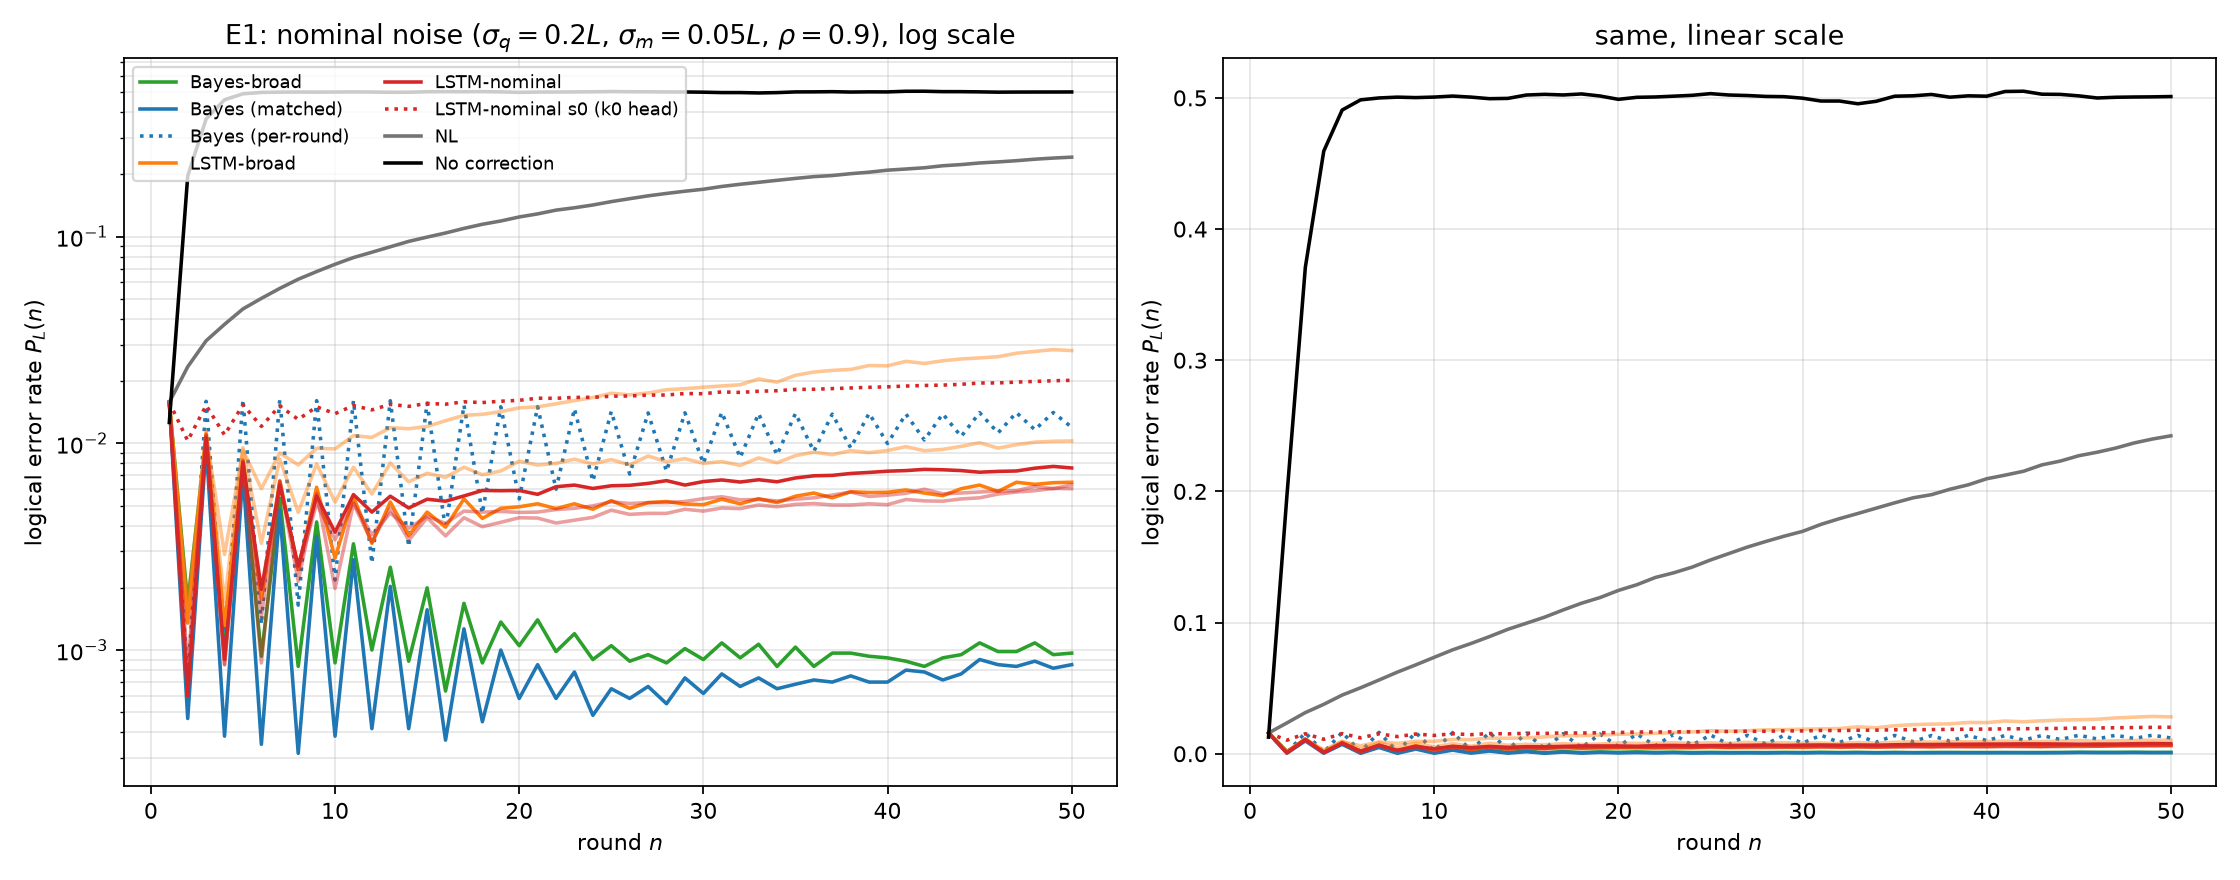
\includegraphics[width=\textwidth]{E1_ler_vs_round.png}
\caption{E1: logical error rate after each round at $\sigma_q=0.2L$,
$\sigma_m=0.05L$, $\rho=0.9$ (\EoneBayesTrials{} trials, common noise).
Faint lines are the individual LSTM seeds.}
\label{fig:e1}
\end{figure}

\begin{table}[H]
\centering\small
\begin{tabular}{lrrrr}
\toprule
Decoder & $P_L(10)$ & $P_L(50)$ & time-avg.\ error & paired diff.\ vs Bayes \\
\midrule
No correction & $0.501$ & $0.501$ & $0.481$ & $+0.480$ {\scriptsize($\pm1\!\times\!10^{-3}$)} \\
NL & $0.073$ & $0.242$ & $0.144$ & $+0.142$ {\scriptsize($\pm2\!\times\!10^{-3}$)} \\
Bayes (matched) & $3.8\!\times\!10^{-4}$ & $8.5\!\times\!10^{-4}$ & $1.5\!\times\!10^{-3}$ & -- \\
Bayes (per-round) & $2.2\!\times\!10^{-3}$ & $0.012$ & $0.011$ & $+9.2\!\times\!10^{-3}$ {\scriptsize($\pm6\!\times\!10^{-4}$)} \\
Bayes-broad & $8.7\!\times\!10^{-4}$ & $9.7\!\times\!10^{-4}$ & $1.9\!\times\!10^{-3}$ & $+3.7\!\times\!10^{-4}$ {\scriptsize($\pm1\!\times\!10^{-4}$)} \\
\textbf{LSTM-nominal (mean of seeds)} & $3.0\!\times\!10^{-3}$ & $6.6\!\times\!10^{-3}$ & $5.5\!\times\!10^{-3}$ & $+4.0\!\times\!10^{-3}$ {\scriptsize($\pm4\!\times\!10^{-4}$)} \\
LSTM-nominal s0 & $3.7\!\times\!10^{-3}$ & $7.6\!\times\!10^{-3}$ & $6.3\!\times\!10^{-3}$ & $+4.8\!\times\!10^{-3}$ {\scriptsize($\pm4\!\times\!10^{-4}$)} \\
LSTM-nominal s1 & $3.4\!\times\!10^{-3}$ & $6.3\!\times\!10^{-3}$ & $5.3\!\times\!10^{-3}$ & $+3.8\!\times\!10^{-3}$ {\scriptsize($\pm4\!\times\!10^{-4}$)} \\
LSTM-nominal s2 & $2.0\!\times\!10^{-3}$ & $6.0\!\times\!10^{-3}$ & $4.9\!\times\!10^{-3}$ & $+3.4\!\times\!10^{-3}$ {\scriptsize($\pm4\!\times\!10^{-4}$)} \\
LSTM-nominal s0 (per-round head) & $0.014$ & $0.020$ & $0.017$ & $+0.015$ {\scriptsize($\pm9\!\times\!10^{-4}$)} \\
\textbf{LSTM-broad (mean of seeds)} & $5.8\!\times\!10^{-3}$ & $0.015$ & $0.010$ & $+8.7\!\times\!10^{-3}$ {\scriptsize($\pm4\!\times\!10^{-4}$)} \\
LSTM-broad s0 & $2.8\!\times\!10^{-3}$ & $6.5\!\times\!10^{-3}$ & $5.4\!\times\!10^{-3}$ & $+3.9\!\times\!10^{-3}$ {\scriptsize($\pm4\!\times\!10^{-4}$)} \\
LSTM-broad s1 & $9.4\!\times\!10^{-3}$ & $0.028$ & $0.017$ & $+0.016$ {\scriptsize($\pm7\!\times\!10^{-4}$)} \\
LSTM-broad s2 & $5.2\!\times\!10^{-3}$ & $0.010$ & $8.2\!\times\!10^{-3}$ & $+6.6\!\times\!10^{-3}$ {\scriptsize($\pm4\!\times\!10^{-4}$)} \\
\bottomrule
\end{tabular}
\caption{E1 at the nominal point. The paired difference is the mean per-trial
difference in time-averaged error from matched Bayes, with its 2-SE
uncertainty. For the seed means the uncertainty shown is that of seed~0.}
\label{tab:e1}
\end{table}

Memory changes the picture completely (Figure~\ref{fig:e1},
Table~\ref{tab:e1}):
\begin{itemize}
  \item \textbf{Nearest lattice} accumulates errors steadily and reaches
    $P_L(50)=\EoneNLLERfifty$.
  \item \textbf{Matched Bayes} reaches $P_L(50)=\EoneBayesLERfifty$, which is
    \EoneBayesEvents{} errors in \EoneBayesTrials{} trials. Its time-averaged
    error is \EoneGain{} times smaller than NL's.
  \item \textbf{Bayes-broad} gets within about 25\% of matched Bayes without
    knowing the parameters ($\EoneBayesBroadMean$ against $\EoneBayesMean$).
  \item \textbf{LSTM-nominal} is trained at this exact point. It reaches a
    time-averaged error of $\EoneLSTMnomMean$, which is \EoneLSTMoverBayes{}
    times that of matched Bayes but still about 26 times better than NL. The
    three seeds lie within about 30\% of each other (3.3--4.2 times matched
    Bayes), a much smaller spread than for the broad seeds.
  \item \textbf{LSTM-broad} reaches $\EoneLSTMbroadMean$ on average, with a
    large spread between seeds: seed~0 matches LSTM-nominal and seed~1 is
    3 times worse. All three broad models finished their full 40-epoch
    schedule, and their validation losses differ little (Table~\ref{tab:training}).
    The spread therefore reflects how differently models trained on the whole
    box handle this particular corner of it, not undertraining.
\end{itemize}

Both ablations show that revising past decisions matters. Bayes restricted to
per-round decisions has error $\EoneBayesPRMean$, about 7 times worse than
full Bayes. The LSTM's per-round head ($k=0$) has error $\EoneLSTMkzeroMean$,
about 2.7 times worse than its cumulative head. Section~\ref{sec:why} explains
the zig-zag in the early rounds.

%----------------------------------------
\subsection{E2: stronger correlation}

\begin{figure}[H]
\centering
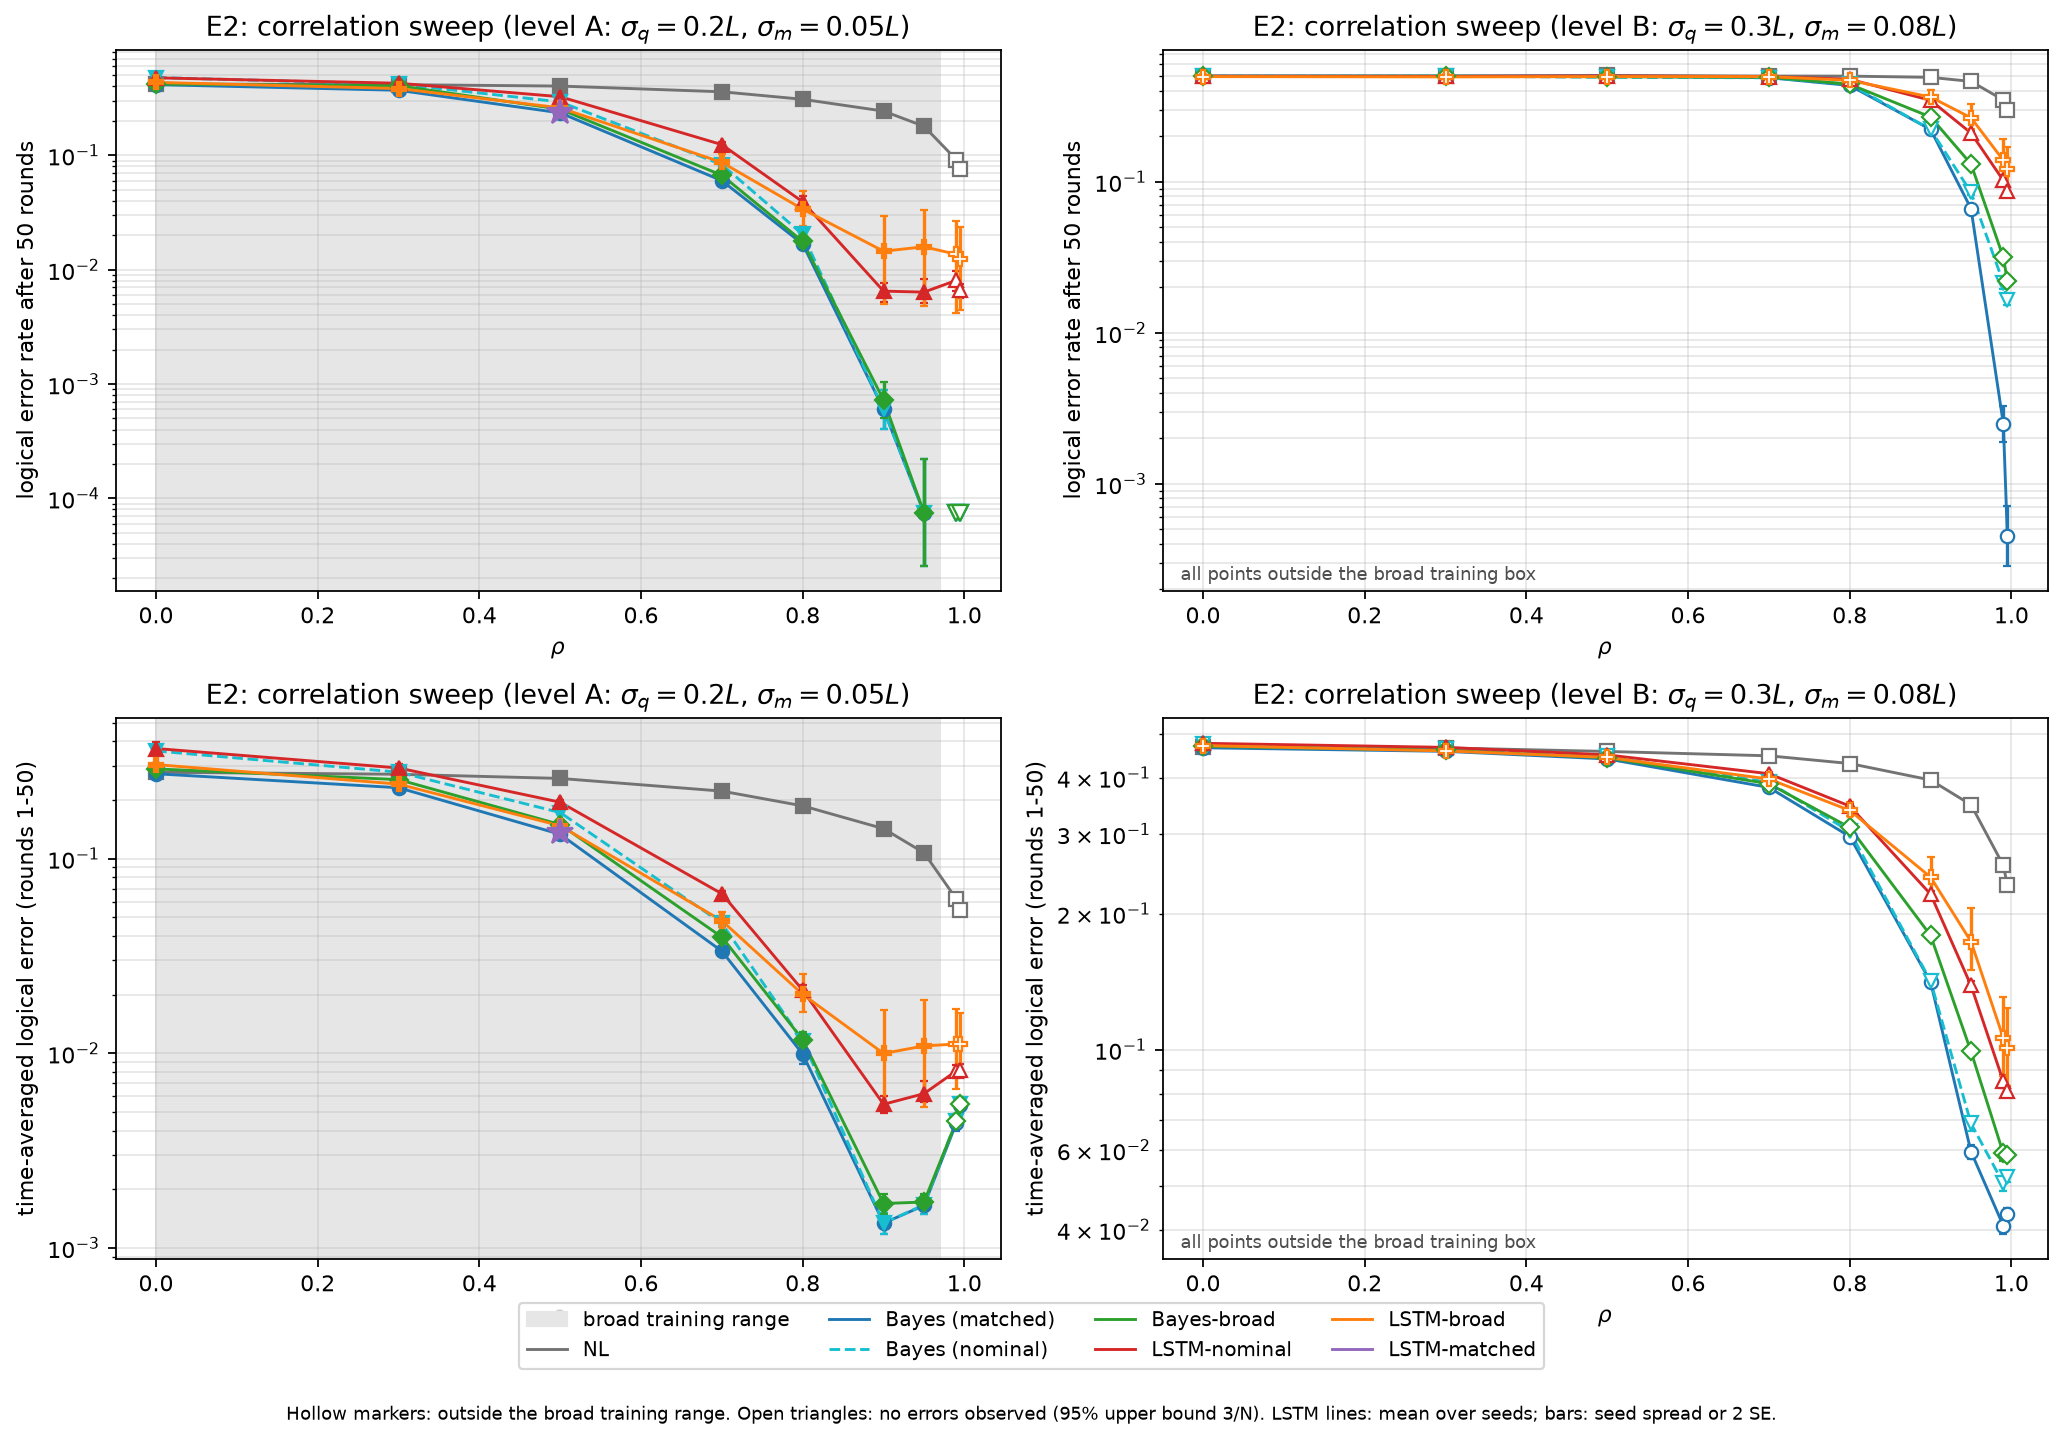
\includegraphics[width=\textwidth]{E2_rho_sweep.png}
\caption{E2: correlation sweep at two noise levels. Top: $P_L(50)$. Bottom:
time-averaged error. The shaded band is the $\rho$ range of the broad
training box. At level~B, $\sigma_q=0.3L$ lies outside the box
($\sigma_m=0.08L$ sits at its upper edge), so every point there is out of
distribution for both broad decoders.}
\label{fig:e2}
\end{figure}

\begin{table}[H]
\centering\small
\resizebox{\textwidth}{!}{\begin{tabular}{lrrrrrrr}
\toprule
$\rho$ & NL & Bayes (matched) & Bayes (nominal) & Bayes-broad & LSTM-nominal & LSTM-broad & LSTM-matched \\
\midrule
0.0 & $0.278$ & $0.273$ & $0.357$ & $0.289$ & $0.368$ & $0.304$ & -- \\
0.3 & $0.271$ & $0.231$ & $0.278$ & $0.255$ & $0.292$ & $0.241$ & -- \\
0.5 & $0.258$ & $0.133$ & $0.172$ & $0.150$ & $0.195$ & $0.147$ & $0.136$ \\
0.7 & $0.222$ & $0.033$ & $0.047$ & $0.040$ & $0.066$ & $0.048$ & -- \\
0.8 & $0.187$ & $9.9\!\times\!10^{-3}$ & $0.012$ & $0.012$ & $0.021$ & $0.020$ & -- \\
0.9 & $0.142$ & $1.3\!\times\!10^{-3}$ & $1.3\!\times\!10^{-3}$ & $1.7\!\times\!10^{-3}$ & $5.5\!\times\!10^{-3}$ & $10.0\!\times\!10^{-3}$ & -- \\
0.95 & $0.107$ & $1.6\!\times\!10^{-3}$ & $1.7\!\times\!10^{-3}$ & $1.7\!\times\!10^{-3}$ & $6.2\!\times\!10^{-3}$ & $0.011$ & -- \\
0.99 & $0.062$ & $4.4\!\times\!10^{-3}$ & $4.5\!\times\!10^{-3}$ & \textit{$4.5\!\times\!10^{-3}$} & $8.1\!\times\!10^{-3}$ & \textit{$0.011$} & -- \\
0.995 & $0.054$ & $5.4\!\times\!10^{-3}$ & $5.5\!\times\!10^{-3}$ & \textit{$5.5\!\times\!10^{-3}$} & $8.2\!\times\!10^{-3}$ & \textit{$0.011$} & -- \\
\bottomrule
\end{tabular}}
\\[4pt]
\resizebox{\textwidth}{!}{\begin{tabular}{lrrrrrrr}
\toprule
$\rho$ & NL & Bayes (matched) & Bayes (nominal) & Bayes-broad & LSTM-nominal & LSTM-broad & LSTM-matched \\
\midrule
0.0 & $0.468$ & $0.466$ & $0.475$ & \textit{$0.469$} & $0.476$ & \textit{$0.471$} & -- \\
0.3 & $0.465$ & $0.457$ & $0.462$ & \textit{$0.460$} & $0.467$ & \textit{$0.458$} & -- \\
0.5 & $0.457$ & $0.440$ & $0.446$ & \textit{$0.443$} & $0.449$ & \textit{$0.443$} & -- \\
0.7 & $0.447$ & $0.380$ & $0.390$ & \textit{$0.388$} & $0.408$ & \textit{$0.397$} & -- \\
0.8 & $0.430$ & $0.296$ & $0.304$ & \textit{$0.310$} & $0.346$ & \textit{$0.338$} & -- \\
0.9 & $0.395$ & $0.141$ & $0.142$ & \textit{$0.179$} & $0.221$ & \textit{$0.241$} & -- \\
0.95 & $0.348$ & $0.060$ & $0.069$ & \textit{$0.099$} & $0.139$ & \textit{$0.173$} & -- \\
0.99 & $0.256$ & $0.041$ & $0.051$ & \textit{$0.059$} & $0.085$ & \textit{$0.106$} & -- \\
0.995 & $0.231$ & $0.043$ & $0.052$ & \textit{$0.058$} & $0.081$ & \textit{$0.101$} & -- \\
\bottomrule
\end{tabular}}
\caption{E2: time-averaged logical error. Top: level A ($\sigma_q=0.2L$,
$\sigma_m=0.05L$). Bottom: level B ($\sigma_q=0.3L$, $\sigma_m=0.08L$).
Italics mark points outside the broad training box.}
\label{tab:e2}
\end{table}

\paragraph{Memory pays off more as correlation grows, up to $\rho\approx0.9$.}
At level~A, matched Bayes improves on NL by a factor of
$\resratio{E2}{A_rho0.0}{NL}$ at $\rho=0$, $\resratio{E2}{A_rho0.7}{NL}$ at
$\rho=0.7$ and $\resratio{E2}{A_rho0.9}{NL}$ at $\rho=0.9$. (Each value is
NL's error divided by matched Bayes's error at that $\rho$.) Beyond
$\rho=0.9$ the factor shrinks ($\resratio{E2}{A_rho0.95}{NL}$ at $\rho=0.95$,
$\resratio{E2}{A_rho0.995}{NL}$ at $\rho=0.995$), because NL's error keeps
falling while matched Bayes's error rises slightly. The small gain at
$\rho=0$ comes from the measurement-noise correlation in~\eqref{eq:z}:
$z_t$ and $z_{t+1}$ share $\nu_t$.

At very high correlation ($\rho\ge0.99$), Bayes shows no errors after
round~50 ($P_L(50)$ is \resfifty{E2}{A_rho0.99}{Bayes (matched)}), yet its
time-averaged error rises again, to $\res{E2}{A_rho0.99}{Bayes (matched)}$.
These errors are not confined to the first rounds. In about 1\% of trials
the logical state is wrong after every odd round and right after every even
round, all the way to round~49. $P_L(50)$ is zero only because round 50 is
even. Section~\ref{sec:why} explains this odd/even pattern.

\paragraph{Wrong memory is worse than no memory.}
At $\rho=0$ every decoder that assumes strong correlation does worse than the
memoryless baseline:
\begin{itemize}
  \item Bayes (nominal), which assumes $\rho=0.9$, has error
    $\res{E2}{A_rho0.0}{Bayes (nominal)}$, against
    $\res{E2}{A_rho0.0}{NL}$ for NL.
  \item LSTM-nominal has error $\res{E2}{A_rho0.0}{LSTM-nominal}$.
\end{itemize}
The broad decoders, which have seen low-$\rho$ noise, stay close to NL there
(Bayes-broad $\res{E2}{A_rho0.0}{Bayes-broad}$, LSTM-broad
$\res{E2}{A_rho0.0}{LSTM-broad}$). Even so, neither matches the matched
filter's $\res{E2}{A_rho0.0}{Bayes (matched)}$.

\paragraph{A matched LSTM is nearly optimal at moderate correlation.}
At $\rho=0.5$, the LSTM trained at exactly that point reaches
$\res{E2}{A_rho0.5}{LSTM-matched}$, which is only
$\resratio{E2}{A_rho0.5}{LSTM-matched}\times$ matched Bayes. LSTM-nominal at
the same point (out of distribution) has error
$\res{E2}{A_rho0.5}{LSTM-nominal}$.

\paragraph{The ML gap tends to grow as errors become rarer.}
Broadly, LSTM-nominal's error relative to matched Bayes grows as Bayes's own
error falls, though not monotonically. Relative to matched Bayes,
LSTM-nominal's error is
\begin{itemize}
  \item $\resratio{E2}{A_rho0.9}{LSTM-nominal}\times$ at $\rho=0.9$ on level~A,
    where Bayes has error $\res{E2}{A_rho0.9}{Bayes (matched)}$;
  \item $\resratio{E2}{B_rho0.9}{LSTM-nominal}\times$ at $\rho=0.9$ on level~B,
    where Bayes has error $\res{E2}{B_rho0.9}{Bayes (matched)}$.
\end{itemize}
The ratio is lower at points where correlation is very high and errors are
more common (A, $\rho=0.99$: $\resratio{E2}{A_rho0.99}{LSTM-nominal}\times$),
and higher at B, $\rho=0.95$ ($\resratio{E2}{B_rho0.95}{LSTM-nominal}\times$).

At level~B the broad decoders are out of distribution in $\sigma_q$, and at
the edge of their training range in $\sigma_m$. For $\rho\ge0.8$ at level~B,
Bayes-broad does worse than Bayes (nominal), e.g.\
$\res{E2}{B_rho0.9}{Bayes-broad}$ against $\res{E2}{B_rho0.9}{Bayes (nominal)}$
at $\rho=0.9$. For $\rho\le0.7$ it is slightly better. Both assume
$\sigma_m'=0.05L$, so the gap comes from Bayes-broad's $(\rho',\sigma_q')$
grid ($\sigma_q'\le0.25L$, against the true $0.3L$).

%----------------------------------------
\subsection{E3 and E4: stronger displacement and measurement noise}

\begin{figure}[H]
\centering
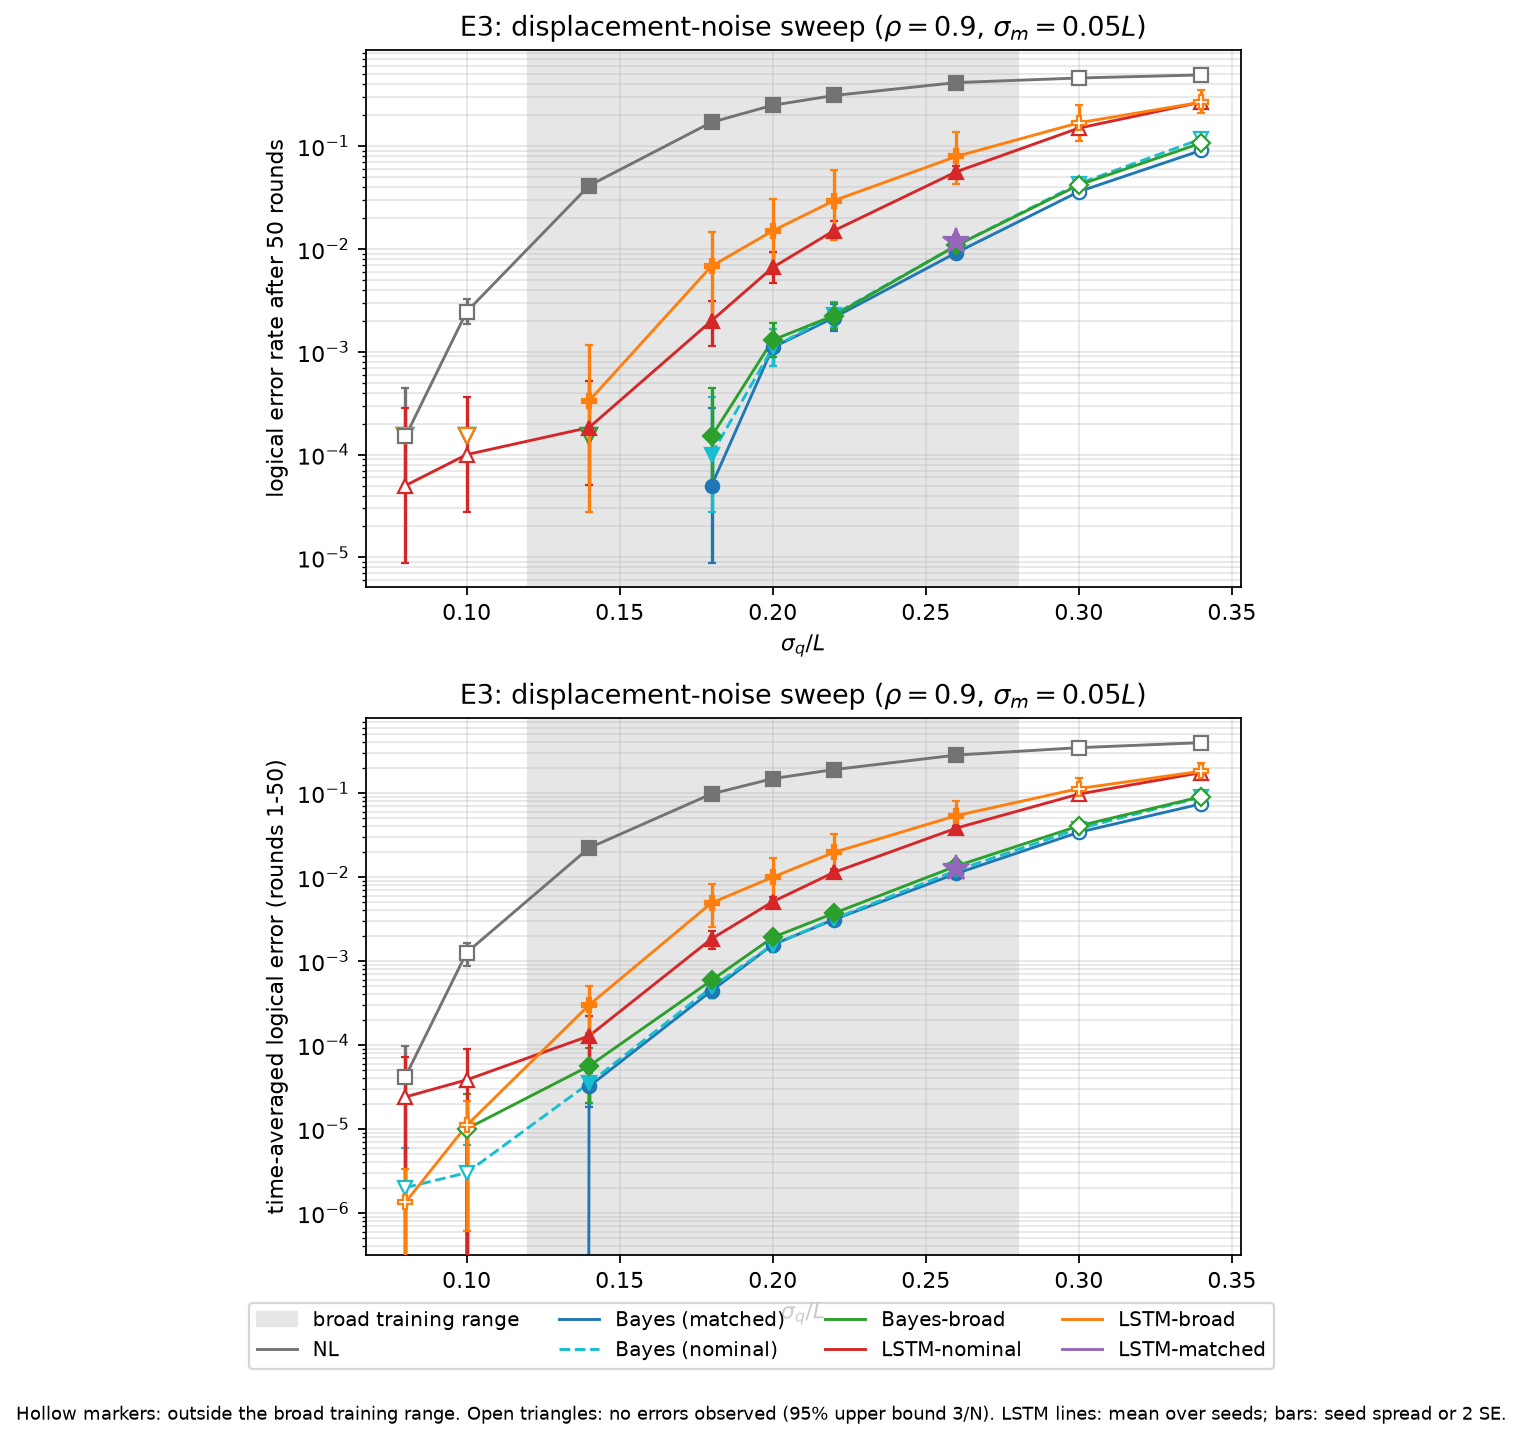
\includegraphics[width=0.95\textwidth]{E3_sigma_q_sweep.png}
\caption{E3: displacement-noise sweep at $\rho=0.9$, $\sigma_m=0.05L$.}
\label{fig:e3}
\end{figure}

\begin{figure}[H]
\centering
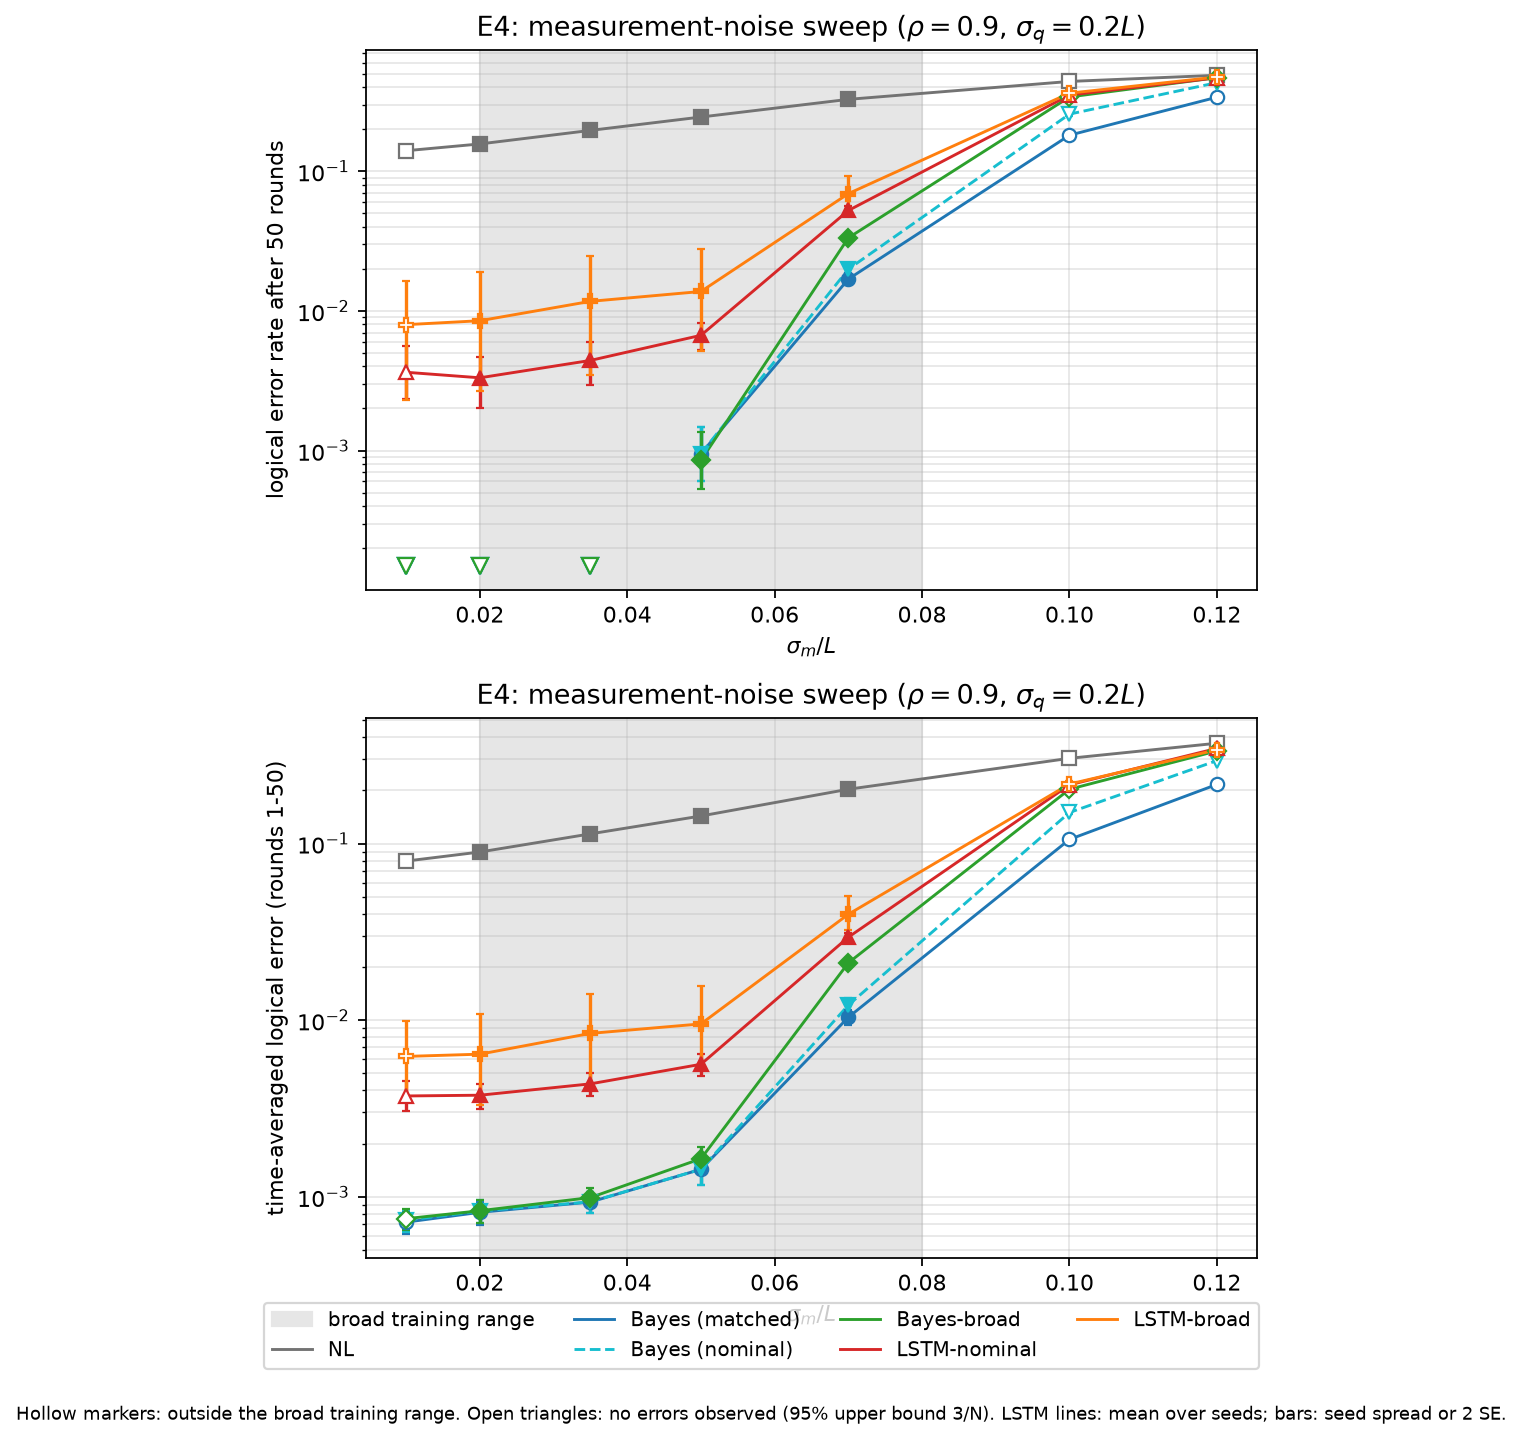
\includegraphics[width=0.95\textwidth]{E4_sigma_m_sweep.png}
\caption{E4: measurement-noise sweep at $\rho=0.9$, $\sigma_q=0.2L$.}
\label{fig:e4}
\end{figure}

\begin{table}[H]
\centering\small
\resizebox{\textwidth}{!}{\begin{tabular}{lrrrrrrr}
\toprule
$\sigma_q/L$ & NL & Bayes (matched) & Bayes (nominal) & Bayes-broad & LSTM-nominal & LSTM-broad & LSTM-matched \\
\midrule
0.08 & $1.5\!\times\!10^{-4}$$^\dagger$ & $<1.5\!\times\!10^{-4}$ & $<1.5\!\times\!10^{-4}$ & \textit{$<1.5\!\times\!10^{-4}$} & $5.0\!\times\!10^{-5}$$^\dagger$ & \textit{$<1.5\!\times\!10^{-4}$} & -- \\
0.1 & $2.4\!\times\!10^{-3}$ & $<1.5\!\times\!10^{-4}$ & $<1.5\!\times\!10^{-4}$ & \textit{$<1.5\!\times\!10^{-4}$} & $1.0\!\times\!10^{-4}$$^\dagger$ & \textit{$<1.5\!\times\!10^{-4}$} & -- \\
0.14 & $0.041$ & $<1.5\!\times\!10^{-4}$ & $<1.5\!\times\!10^{-4}$ & $<1.5\!\times\!10^{-4}$ & $1.8\!\times\!10^{-4}$ & $3.3\!\times\!10^{-4}$ & -- \\
0.18 & $0.170$ & $5.0\!\times\!10^{-5}$$^\dagger$ & $1.0\!\times\!10^{-4}$$^\dagger$ & $1.5\!\times\!10^{-4}$$^\dagger$ & $2.0\!\times\!10^{-3}$ & $6.8\!\times\!10^{-3}$ & -- \\
0.2 & $0.249$ & $1.1\!\times\!10^{-3}$ & $1.1\!\times\!10^{-3}$ & $1.3\!\times\!10^{-3}$ & $6.6\!\times\!10^{-3}$ & $0.015$ & -- \\
0.22 & $0.310$ & $2.1\!\times\!10^{-3}$ & $2.3\!\times\!10^{-3}$ & $2.2\!\times\!10^{-3}$ & $0.015$ & $0.029$ & -- \\
0.26 & $0.414$ & $9.2\!\times\!10^{-3}$ & $0.011$ & $0.011$ & $0.056$ & $0.079$ & $0.012$ \\
0.3 & $0.459$ & $0.036$ & $0.043$ & \textit{$0.042$} & $0.150$ & \textit{$0.168$} & -- \\
0.34 & $0.492$ & $0.091$ & $0.117$ & \textit{$0.107$} & $0.268$ & \textit{$0.267$} & -- \\
\bottomrule
\end{tabular}}
\\[4pt]
\resizebox{0.9\textwidth}{!}{\begin{tabular}{lrrrrrr}
\toprule
$\sigma_m/L$ & NL & Bayes (matched) & Bayes (nominal) & Bayes-broad & LSTM-nominal & LSTM-broad \\
\midrule
0.01 & $0.140$ & $<1.5\!\times\!10^{-4}$ & $<1.5\!\times\!10^{-4}$ & \textit{$<1.5\!\times\!10^{-4}$} & $3.6\!\times\!10^{-3}$ & \textit{$8.0\!\times\!10^{-3}$} \\
0.02 & $0.157$ & $<1.5\!\times\!10^{-4}$ & $<1.5\!\times\!10^{-4}$ & $<1.5\!\times\!10^{-4}$ & $3.3\!\times\!10^{-3}$ & $8.5\!\times\!10^{-3}$ \\
0.035 & $0.196$ & $<1.5\!\times\!10^{-4}$ & $<1.5\!\times\!10^{-4}$ & $<1.5\!\times\!10^{-4}$ & $4.4\!\times\!10^{-3}$ & $0.012$ \\
0.05 & $0.244$ & $9.5\!\times\!10^{-4}$ & $9.5\!\times\!10^{-4}$ & $8.5\!\times\!10^{-4}$ & $6.7\!\times\!10^{-3}$ & $0.014$ \\
0.07 & $0.327$ & $0.017$ & $0.020$ & $0.033$ & $0.052$ & $0.069$ \\
0.1 & $0.440$ & $0.181$ & $0.257$ & \textit{$0.340$} & $0.351$ & \textit{$0.362$} \\
0.12 & $0.487$ & $0.339$ & $0.431$ & \textit{$0.468$} & $0.467$ & \textit{$0.473$} \\
\bottomrule
\end{tabular}}
\caption{E3 (top) and E4 (bottom): $P_L(50)$; 20{,}000 trials per point.}
\label{tab:e34}
\end{table}

\paragraph{Displacement noise.}
All errors rise steeply with $\sigma_q$ (Figure~\ref{fig:e3}). Wherever
errors are resolved ($\sigma_q\ge0.14L$), the ordering of the nominal and
broad decoders never changes: matched Bayes is best, then Bayes (nominal) and
Bayes-broad, then LSTM-nominal and LSTM-broad, then NL. The exception is the
LSTM trained at $\sigma_q=0.26L$, which is level with the model-based filters
at that point. The model-based filters are remarkably
insensitive to a wrong $\sigma_q$ here. Bayes (nominal) assumes
$\sigma_q=0.2L$ and is within 20\% of matched Bayes up to $\sigma_q=0.34L$.

At $\sigma_q=0.26L$ the matched LSTM (error
$\res{E3}{sq0.26}{LSTM-matched}$) is again close to matched Bayes
($\resratio{E3}{sq0.26}{LSTM-matched}\times$). LSTM-nominal is
$\resratio{E3}{sq0.26}{LSTM-nominal}\times$ matched Bayes at that point.

\paragraph{Measurement noise.}
Measurement noise is the harder axis (Figure~\ref{fig:e4}). Once $\sigma_m$
reaches about $0.07L$, the syndrome no longer pins down the error well, and
every decoder degrades quickly. At $\sigma_m=0.10L$:
\begin{itemize}
  \item Bayes (nominal), which assumes $\sigma_m=0.05L$, has error
    $\res{E4}{sm0.1}{Bayes (nominal)}$, against
    $\res{E4}{sm0.1}{Bayes (matched)}$ for matched Bayes.
  \item Bayes-broad, whose components all assume $\sigma_m'=0.05L$, has error
    $\res{E4}{sm0.1}{Bayes-broad}$. That is still about 6\% better than the
    LSTMs (LSTM-broad $\res{E4}{sm0.1}{LSTM-broad}$, LSTM-nominal
    $\res{E4}{sm0.1}{LSTM-nominal}$), but most of its earlier lead is gone.
\end{itemize}

%----------------------------------------
\subsection{E5: Bayes with a mis-specified model}

\begin{figure}[H]
\centering
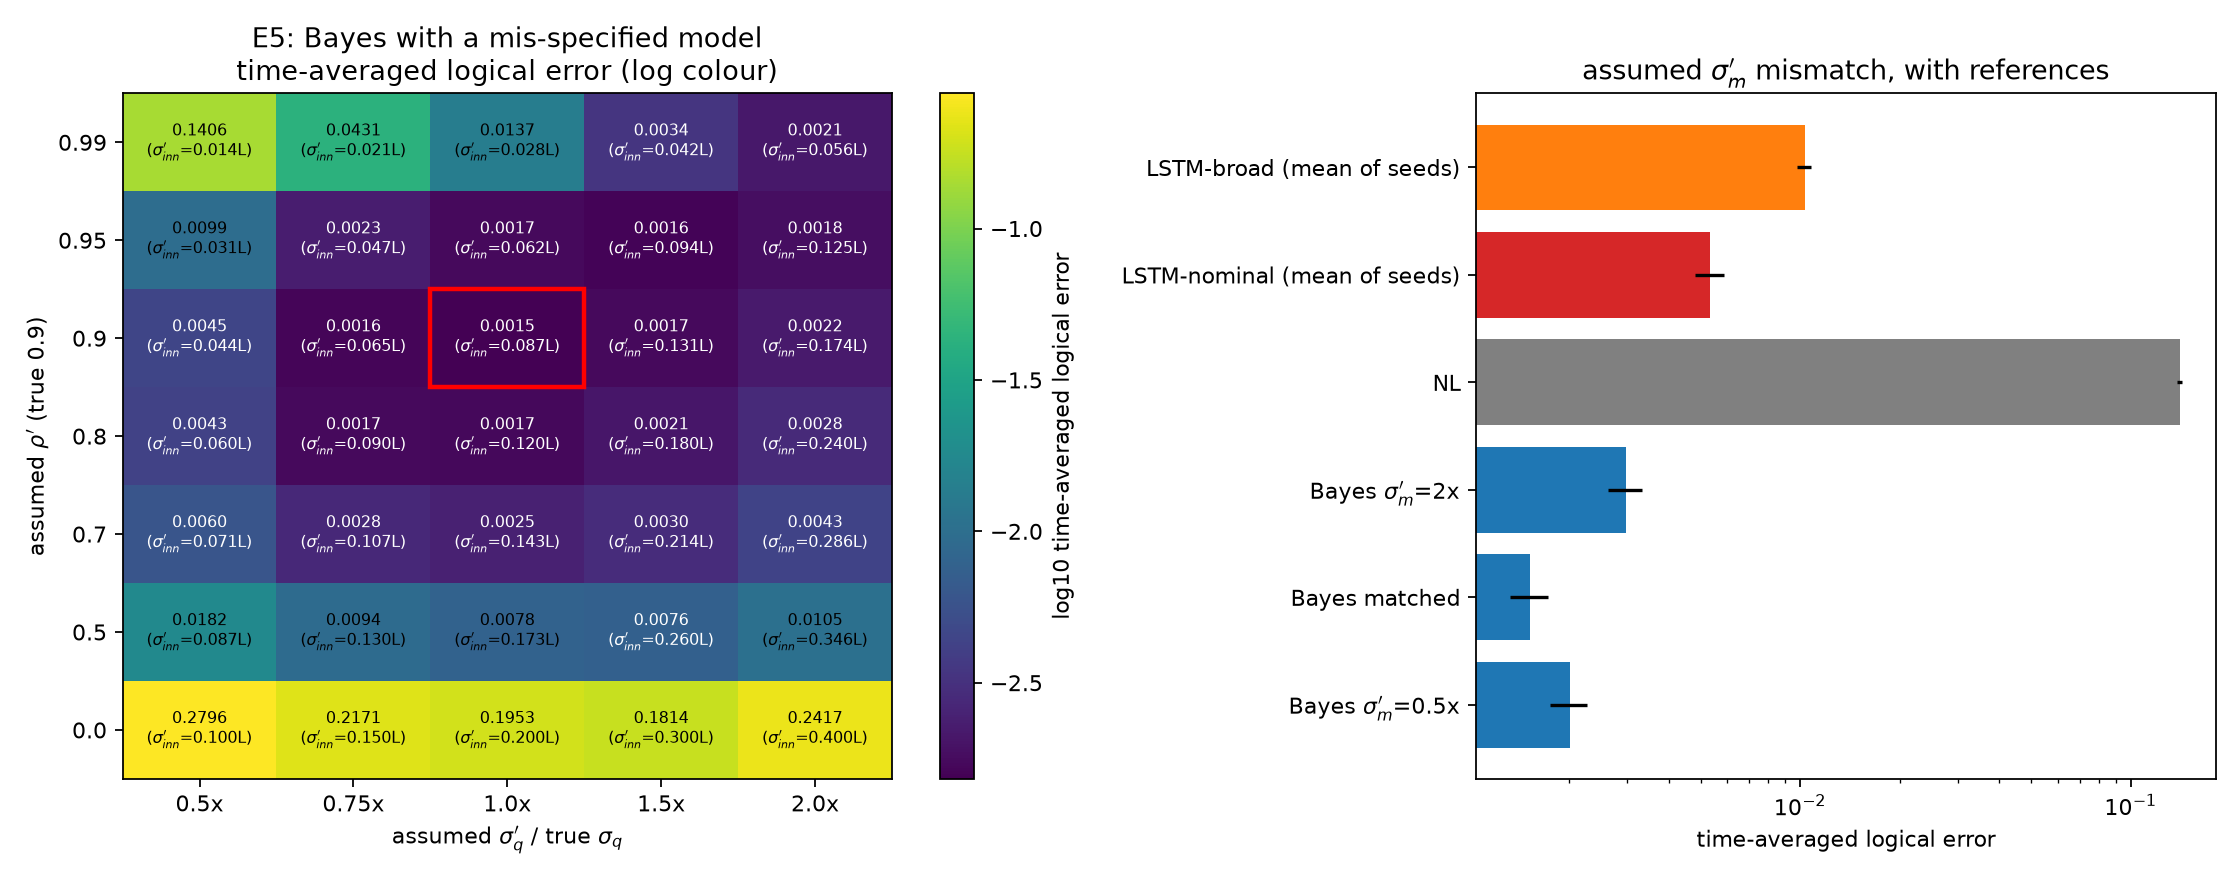
\includegraphics[width=\textwidth]{E5_mismatch.png}
\caption{E5: time-averaged error of Bayes filters with wrong assumed
parameters, at the nominal truth (\EfiveTrials{} trials, common noise). Each
cell gives the innovation standard deviation implied by the assumed
parameters; the true value is $0.087L$ (red box).}
\label{fig:e5}
\end{figure}

\begin{table}[H]
\centering\small
\begin{tabular}{lrrrrr}
\toprule
$\rho'$ \textbackslash{} $\sigma_q'/\sigma_q$ & 0.5 & 0.75 & 1.0 & 1.5 & 2.0 \\
\midrule
0.0 & $0.280$ & $0.217$ & $0.195$ & $0.181$ & $0.242$ \\
0.5 & $0.018$ & $9.4\!\times\!10^{-3}$ & $7.8\!\times\!10^{-3}$ & $7.6\!\times\!10^{-3}$ & $0.010$ \\
0.7 & $6.0\!\times\!10^{-3}$ & $2.8\!\times\!10^{-3}$ & $2.5\!\times\!10^{-3}$ & $3.0\!\times\!10^{-3}$ & $4.3\!\times\!10^{-3}$ \\
0.8 & $4.3\!\times\!10^{-3}$ & $1.7\!\times\!10^{-3}$ & $1.7\!\times\!10^{-3}$ & $2.1\!\times\!10^{-3}$ & $2.8\!\times\!10^{-3}$ \\
0.9 & $4.5\!\times\!10^{-3}$ & $1.6\!\times\!10^{-3}$ & \textbf{$1.5\!\times\!10^{-3}$} & $1.7\!\times\!10^{-3}$ & $2.2\!\times\!10^{-3}$ \\
0.95 & $9.9\!\times\!10^{-3}$ & $2.3\!\times\!10^{-3}$ & $1.7\!\times\!10^{-3}$ & $1.6\!\times\!10^{-3}$ & $1.8\!\times\!10^{-3}$ \\
0.99 & $0.141$ & $0.043$ & $0.014$ & $3.4\!\times\!10^{-3}$ & $2.1\!\times\!10^{-3}$ \\
\bottomrule
\end{tabular}
\caption{E5: time-averaged error against the assumed $\rho'$ (rows) and
$\sigma_q'/\sigma_q$ (columns). The truth is $\rho=0.9$; the matched cell is
in bold.}
\label{tab:e5}
\end{table}

The filter tolerates moderate mismatch well. Every model with
$0.8\le\rho'\le0.95$ and $0.75\le\sigma_q'/\sigma_q\le1.5$ stays within
$1.6\times$ of the matched error. Near the true correlation, the assumed
innovation standard deviation $\sigma_q'\sqrt{1-\rho'^2}$ (printed in each
cell) is a useful guide, but it does not determine the error by itself:
\begin{itemize}
  \item \textbf{Overestimating it by raising $\sigma_q'$ is cheap.} With
    $\sigma_q'=2\sigma_q$ the error only rises to $\EfiveSqTwoMean$. Getting
    a similar overestimate by lowering $\rho'$ costs much more: $\rho'=0.5$
    gives $\EfiveRhoHalfMean$.
  \item \textbf{Underestimating it is expensive.} A filter that thinks the
    displacement is more predictable than it is becomes overconfident. With
    $\rho'=0.99$ the error is $\EfiveRhoHighMean$; with $\rho'=0.99$ and
    $\sigma_q'=0.5\sigma_q$ it collapses to NL's level
    ($\res{E5}{nominal}{Bayes rho'=0.99 sq'x0.5}$).
  \item \textbf{Assuming no correlation ($\rho'=0$)} is worse than NL
    ($\EfiveRhoZeroMean$ against $\EfiveNLMean$). The filter then commits to
    the wrong cell whenever the current syndrome is ambiguous, and it never
    uses the history that would have resolved it.
  \item \textbf{A wrong measurement noise} costs up to about a factor of 2
    at the two values tested ($\sigma_m'=0.5\sigma_m$: $\EfiveSmHalfMean$;
    $\sigma_m'=2\sigma_m$: $\EfiveSmTwoMean$).
\end{itemize}
Measured against this scale, LSTM-nominal ($\EfiveLSTMnomMean$, at its own
training point) is about as good as a Bayes filter with a moderately wrong
model, e.g.\ $\rho'=0.7$ and $\sigma_q'=0.5\sigma_q$. Many mis-specified
filters beat it, and some severely mis-specified ones do not.

%----------------------------------------
\subsection{E6: regime-switching noise}

\begin{figure}[H]
\centering
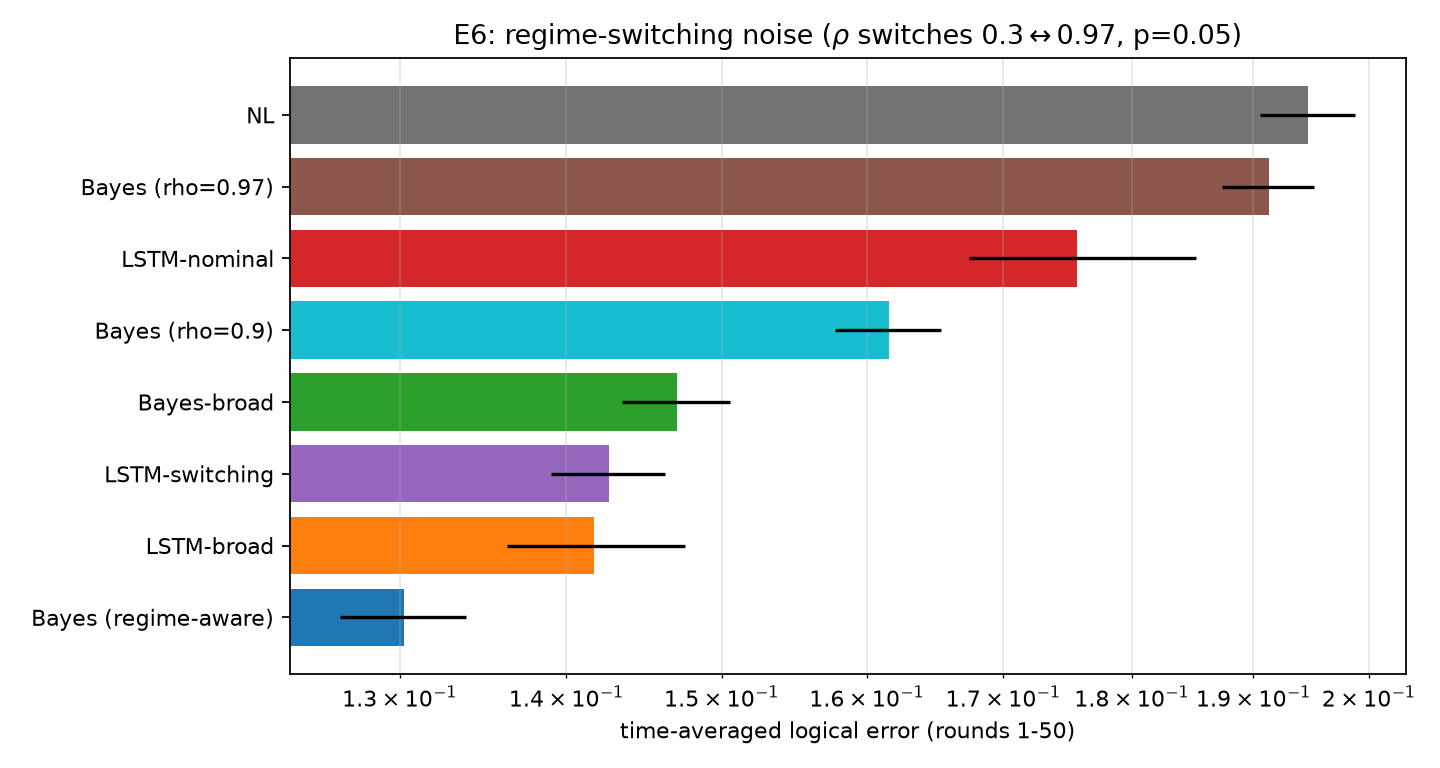
\includegraphics[width=0.75\textwidth]{E6_switching.png}
\caption{E6: the correlation switches between $\rho=0.3$ and $\rho=0.97$ with
probability 0.05 per round. Bars show the 2-SE test-noise uncertainty plus,
for the LSTM seed means, the spread between seeds.}
\label{fig:e6}
\end{figure}

\begin{table}[H]
\centering\small
\begin{tabular}{lrrr}
\toprule
Decoder & $P_L(10)$ & $P_L(50)$ & time-avg.\ error \\
\midrule
NL & $0.101$ & $0.320$ & $0.195$ \\
Bayes (regime-aware) & $0.061$ & $0.226$ & $0.130$ \\
Bayes (rho=0.9) & $0.081$ & $0.269$ & $0.162$ \\
Bayes (rho=0.97) & $0.099$ & $0.312$ & $0.191$ \\
Bayes-broad & $0.065$ & $0.251$ & $0.147$ \\
LSTM-nominal (mean of seeds) & $0.091$ & $0.290$ & $0.176$ {\scriptsize[0.17,\,0.18]} \\
LSTM-broad (mean of seeds) & $0.065$ & $0.246$ & $0.142$ {\scriptsize[0.14,\,0.14]} \\
LSTM-switching & $0.068$ & $0.247$ & $0.143$ \\
\bottomrule
\end{tabular}
\caption{E6: switching noise (20{,}000 trials, common noise).}
\label{tab:e6}
\end{table}

Under noise whose correlation switches between regimes, the decoder that
models the switching is best: regime-aware Bayes has error
$\EsixBayesregimeawareMean$, against $\EsixNLMean$ for NL. This is the
setting where the proposal expected machine learning to help when the
Bayesian model is wrong, and it does. LSTM-broad ($\EsixLSTMbroadMean$) beats
every \emph{fixed-model} Bayes filter:
\begin{itemize}
  \item $\rho=0.9$: $\EsixBayesrhozeronineMean$;
  \item $\rho=0.97$: $\EsixBayesrhozeroninesevenMean$, worse than LSTM-nominal;
  \item Bayes-broad: $\EsixBayesbroadMean$.
\end{itemize}
An LSTM trained on the switching noise itself ($\EsixLSTMswitchingMean$) is
no better than the broad one. So the LSTM's advantage over the fixed filters
here comes from having seen varied correlations, not from learning this
specific process.

%----------------------------------------
\subsection{E7: computational cost}

\begin{table}[H]
\centering\small
\begin{tabular}{llrrr}
\toprule
Decoder & device & batch & ms / round & trial-rounds / s \\
\midrule
Bayes (matched) & cuda & 1 & 3.43 & 292 \\
Bayes (matched) & cuda & 4096 & 13.3 & 3.08e+05 \\
Bayes-broad & cuda & 1 & 22.6 & 44.2 \\
Bayes-broad & cuda & 4096 & 122 & 3.36e+04 \\
LSTM-nominal s0 & cuda & 1 & 1.5 & 668 \\
LSTM-nominal s0 & cuda & 4096 & 13 & 3.15e+05 \\
NL & cpu & 1 & 0.00644 & 1.55e+05 \\
NL & cpu & 512 & 0.0188 & 2.72e+07 \\
Bayes (matched) & cpu & 1 & 0.873 & 1.15e+03 \\
Bayes (matched) & cpu & 512 & 53.1 & 9.65e+03 \\
Bayes-broad & cpu & 1 & 4.77 & 210 \\
Bayes-broad & cpu & 512 & 437 & 1.17e+03 \\
LSTM-nominal s0 & cpu & 1 & 0.944 & 1.06e+03 \\
LSTM-nominal s0 & cpu & 512 & 1.93 & 2.66e+05 \\
\bottomrule
\end{tabular}
\caption{E7: decoding cost per round, measured on an otherwise idle
\GPUname{} and the host CPU. Batch 1 gives the latency of one decoder instance;
the large batch gives throughput.}
\label{tab:e7}
\end{table}

For a single trial on the CPU, NL takes microseconds, while matched Bayes and
the LSTM both take about a millisecond per round
($\tim{Bayes (matched)}{cpu}{1}{latency}$ and
$\tim{LSTM-nominal s0}{cpu}{1}{latency}$~ms). Batched, the picture differs by
device:
\begin{itemize}
  \item \textbf{GPU:} the LSTM and the grid filter have similar throughput
    ($\tim{LSTM-nominal s0}{cuda}{4096}{throughput}$ against
    $\tim{Bayes (matched)}{cuda}{4096}{throughput}$ trial-rounds/s).
  \item \textbf{CPU:} the LSTM's throughput is about 27 times the filter's.
\end{itemize}
Batched, Bayes-broad (8 components) costs as much as 8--9 single filters; for
a single trial it costs about 5.5--6.6 times one filter. Training each LSTM
took 6--11~minutes of wall time for 40 epochs, measured while the GPU was
shared with the Bayes evaluations (Table~\ref{tab:training}). The filter's cost grows with
the grid ($n_x\times n_\varepsilon$ cells per trial) and would grow further
with more hidden variables, e.g.\ for regimes or the $p$ quadrature. The
LSTM's cost is fixed by its size.


%-------------------------------------------------------------------
\section{Why: diagnostics}\label{sec:why}

\begin{figure}[H]
\centering
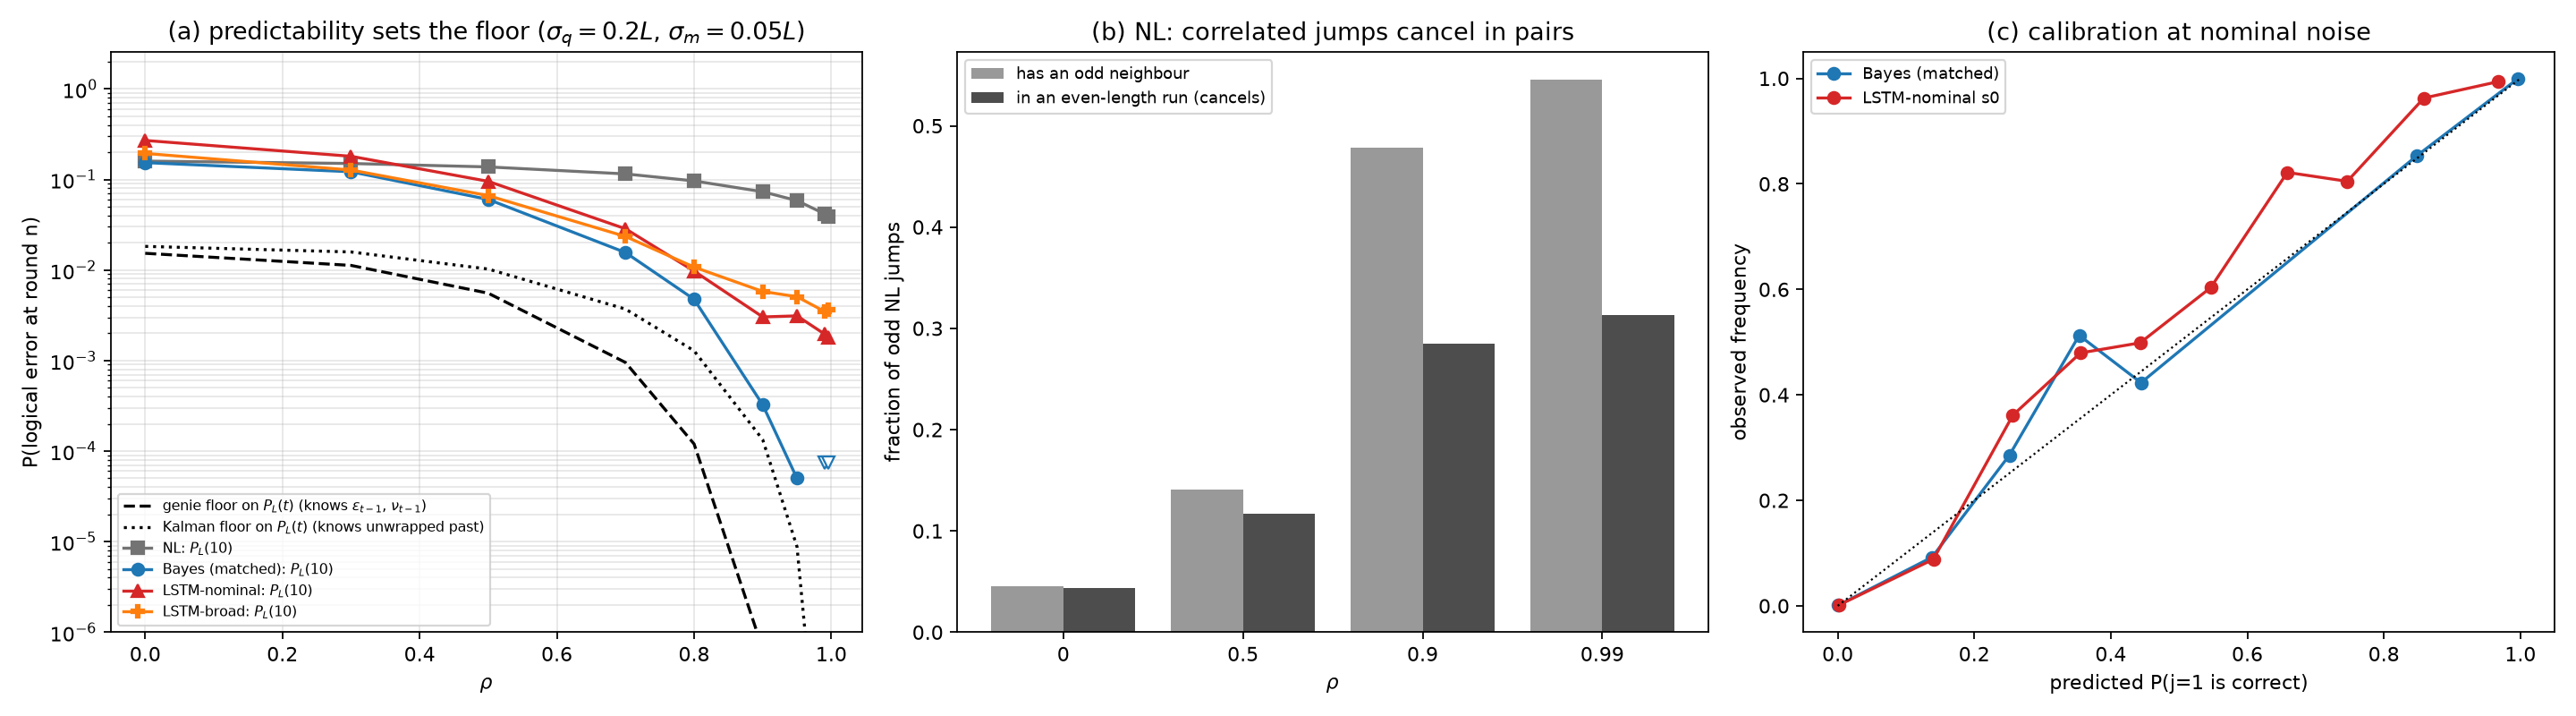
\includegraphics[width=\textwidth]{E8_diagnostics.png}
\caption{E8 diagnostics. (a) $P_L(10)$ against $\rho$ (level~A), with two
analytic floors: a genie that knows $\varepsilon_{t-1}$ and $\nu_{t-1}$, and
the optimal (Kalman) predictor given the \emph{unwrapped} past. (b) NL's odd
jumps cluster as correlation grows. (c) Calibration of the per-round
probability $P(j_t=1\text{ is correct})$ at the nominal point.}
\label{fig:e8}
\end{figure}

\paragraph{Why memory helps: predictability.}
With $c_t=s_t+j_tL$, the only uncertainty in round $t$ is which lattice cell
$z_t=\varepsilon_t+\nu_t-\nu_{t-1}$ fell into~\eqref{eq:z}. The history
predicts $\varepsilon_t$ with an innovation standard deviation of
$\sigma_q\sqrt{1-\rho^2}$, which shrinks from $\sigma_q$ at $\rho=0$ to almost
nothing at $\rho\to1$. Figure~\ref{fig:e8}(a) shows that the per-round floors
follow this.
\begin{itemize}
  \item A decoder that knew the unwrapped past would err in about 1.8\% of
    rounds at $\rho=0$, but only about $10^{-4}$ at $\rho=0.9$.
  \item Matched Bayes tracks this floor at high $\rho$. At $\rho=0.9$ its
    $P_L(10)$ is within a factor of about 3 of the Kalman floor, which knows
    strictly more than the decoder.
  \item At low $\rho$ the gap is wide because errors accumulate over the
    10~rounds.
\end{itemize}

\paragraph{Why NL also improves with $\rho$.}
NL's per-round jump probability does not depend on $\rho$
(\nolinkurl{docs/sim_validation}), yet its $P_L(50)$ falls as $\rho$ grows. The
reason is that correlated jumps come in runs (Figure~\ref{fig:e8}(b)):
\begin{itemize}
  \item at $\rho=0$, \EpairZero{} of odd jumps have an odd neighbour;
  \item at $\rho=0.9$, \EpairNominal{} do, and \EcancelNominal{} sit in
    even-length runs whose parities cancel.
\end{itemize}
This is the same effect reported in the simulator validation.

\paragraph{Why the early rounds zig-zag.}
When $\rho$ is close to 1, a large $\varepsilon$ near $\pm L/2$ is nearly
frozen. The first syndrome cannot tell which cell it is in. If the decoder
guesses wrong, the error then flips the logical state every round until the
evidence (the slow drift of $\varepsilon$) resolves it. This is the odd/even
pattern of Figure~\ref{fig:e1}, and the $\rho\to1$ limit derived in
\texttt{docs/sim\_validation}. Bayes resolves most such cases within a few
rounds. At $\rho\ge0.99$, however, about 1\% of trials have a displacement so
close to the cell boundary that the slow drift never settles it, and those
trials stay wrong after every odd round. That is why $P_L(50)$ (an even round)
vanishes there while the time-averaged error does not.

\paragraph{Why revising decisions matters.}
A decision that looked right given $s_1..s_t$ can be shown wrong by
$s_{t+1},s_{t+2},\dots$ once the drift of $\varepsilon$ becomes visible. The
cumulative rule $J_t=\hat K_t$ undoes such mistakes, while per-round rules
lock them in. The ablations quantify this at the nominal point:
\begin{itemize}
  \item Bayes: $\ErevBayes$ (cumulative) against $\ErevBayesPR$ (per-round);
  \item LSTM: $\ErevLSTM$ against $\ErevLSTMkzero$.
\end{itemize}
In every LSTM, validation selected the cumulative head
(Table~\ref{tab:training}).

\paragraph{Where the LSTM loses to Bayes.}
At the nominal point, the two decoders disagree in only $\EdiagDisagree$ of
trial-rounds. When they disagree, Bayes is right \EdiagBayesRight\% of the
time, and its posterior is almost always decisive there; it is the LSTM's
output that sits close to 0.5. The LSTM's errors are therefore concentrated
in rare rounds that the exact posterior settles clearly but the network has
not learned: rounds with an odd nearest-lattice jump, where these decisions
arise, are only about 2\% of the training data.

This fits the pattern in E2 and E3: the LSTM approaches Bayes where errors
are common (matched LSTM within 2--17\% at $\rho=0.5$ and at
$\sigma_q=0.26L$), and falls behind where they are rare. The LSTM's
probabilities are also biased low (Figure~\ref{fig:e8}(c)). From a predicted
value of about 0.25 upwards, observed frequencies exceed its predicted
$P(j_t=1)$ by up to about 0.15, so it is under-confident above 0.5 and
over-confident towards $j_t=0$ between 0.25 and 0.5. Bayes is approximately
calibrated.

\paragraph{Generalisation over time.}
Run for 200 rounds, all memory decoders keep working well past their
50-round training length (Figure~\ref{fig:e8h}). Errors accumulate slowly:
\begin{itemize}
  \item matched Bayes: $\EhzBayesFifty\to\EhzBayesTwohundred$;
  \item LSTM-nominal: $\EhzLSTMnomFifty\to\EhzLSTMnomTwohundred$;
  \item NL: $\EhzNLFifty\to\EhzNLTwohundred$.
\end{itemize}

\begin{figure}[H]
\centering
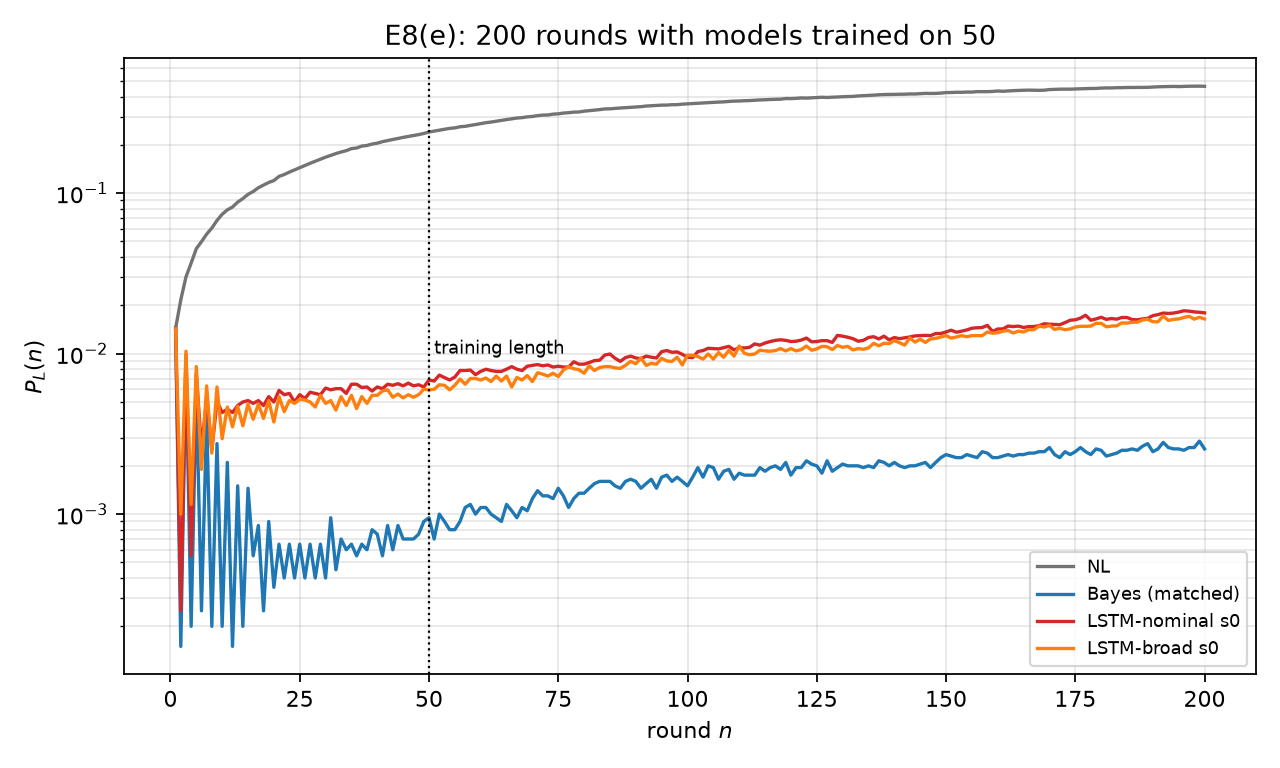
\includegraphics[width=0.62\textwidth]{E8_horizon.png}
\caption{E8(e): 200 rounds at the nominal point; the LSTMs were trained on
50-round sequences.}
\label{fig:e8h}
\end{figure}


%-------------------------------------------------------------------
\section{Discussion: when does each method win?}\label{sec:discussion}

\paragraph{Memory helps, and more so the more correlated the noise.}
Once $\rho\gtrsim0.5$, every decoder in the parameter sweeps (E2--E4) beats
nearest lattice, by up to two orders of magnitude at $\rho\approx0.9$. Badly
mis-specified filters (E5) are the exception. The gain follows the
predictability of the next displacement, $\sigma_q\sqrt{1-\rho^2}$
(Section~\ref{sec:why}). Much of it, though not most, comes from being able
to \emph{revise} earlier decisions. At the nominal point, predicting the next
displacement alone gives a factor of about 13 for Bayes (about 9 for the
LSTM), and revision adds a further factor of about 7 (about 2.7 for the LSTM).

\paragraph{When the model is right, Bayes wins.}
With the correct noise model, the grid filter is the optimal syndrome-only
decoder for this action set, and it was best at every test point. The best
LSTMs come within 2--17\% of it where logical errors are common (matched
models at $\rho=0.5$: 2\%; at $\sigma_q=0.26L$: 17\%). They fall 3--4 times
behind where errors are rare (the nominal point): the decisive rounds are
rare in the training data, and the network has not learned them.

\paragraph{When the model is moderately wrong, Bayes usually still wins.}
A filter whose assumed parameters are moderately off loses little: every
model with $0.8\le\rho'\le0.95$ and $0.75\le\sigma_q'/\sigma_q\le1.5$ stays
within $1.6\times$ of the matched error. Overestimating $\sigma_q$ is cheap.
Underestimating the innovation noise, lowering $\rho'$ substantially, or
ignoring the correlation is expensive, and can be worse than no memory at all
(E5).

In the parameter sweeps, the fixed nominal filter stayed close to matched
Bayes over a wide range of $\sigma_q$ and for $\rho\ge0.8$. Averaged over
LSTM seeds, its error was at or below that of the nominally trained LSTM at
every sweep point; at $\rho=0$ the two were within the LSTM seed spread.

A Bayesian average over a coarse grid of models (Bayes-broad) matched or beat
the broadly trained LSTM at most test points, including most of level~B,
where both are out of distribution. The exceptions are weak-to-moderate
correlation inside the training box: the LSTM was better at level~A with
$\rho=0.3$ for all three seeds, and slightly better at $\rho=0.5$.

\paragraph{When the model is structurally wrong, ML helps.}
Under regime-switching correlation (E6), every fixed-model filter is
mis-specified, and the LSTM trained on varied noise beat all of them. Only a
filter that models the switching did better. This is the clearest support in
our data for the proposal's hypothesis that machine learning helps when the
Bayesian model is inaccurate. The advantage came from training on varied
correlations rather than on the switching process itself.

\paragraph{Generalisation needs varied training.}
\begin{itemize}
  \item A network trained at one point degrades away from it. At $\rho=0$ it
    is worse than NL on average over seeds, because it applies memory that is
    not there.
  \item Training on a broad box removes most of that failure, at the cost of
    some in-distribution performance and a larger spread between seeds.
  \item The same holds for Bayes: a single assumed model is fragile in the
    same places, and averaging over models removes most of the problem. At
    $\rho=0$, Bayes-broad is still slightly worse than NL.
\end{itemize}

\paragraph{Cost.}
On a GPU, both memory decoders process about $3\times10^5$ trial-rounds per
second, with a latency of a few milliseconds per round. On a CPU, the
single-trial latency is similar (about 0.9~ms per round for both), but for
batched decoding the LSTM's throughput is about 27 times the grid filter's.
The filter's cost grows with the number of hidden variables, which favours
learned decoders for richer noise models. The LSTM, in turn, needs training
data and about 6--11 minutes of GPU time per model.

\paragraph{Answer to the research question.}
In this setting, machine learning did not outperform a correctly specified
Bayesian filter, and it rarely outperformed a mildly mis-specified one. The
exception is a model-averaged filter at weak correlation. A broadly trained
LSTM is nevertheless a robust, cheap and assumption-light decoder:
\begin{itemize}
  \item it beats nearest-lattice decoding by large factors under correlated
    noise;
  \item it beats mis-specified filters when the true noise is structurally
    different from what the filter assumes.
\end{itemize}


%-------------------------------------------------------------------
\section{Limitations and future work}\label{sec:limits}

\paragraph{Model scope.}
\begin{itemize}
  \item \emph{One quadrature, classical shifts.} Everything is in the $q$
    quadrature with classical shifts on an ideal (infinite-energy) code.
    Finite-energy envelopes, $p$-quadrature noise, photon loss and ancilla
    noise inside the syndrome-extraction circuit are not modelled. The
    finite-$\Delta$ state in \texttt{quantum/encoding.py} is the natural next
    step for checking the shift model.
  \item \emph{Discrete corrections.} Decoders choose only the parity $j_t$ of
    a correction $s_t+j_tL$. A decoder that also estimates $\nu_t$ and applies
    a continuous fine correction could reduce the residual further. This
    restriction is what makes the syndrome history independent of the
    decoder (Section~\ref{sec:model}), so it simplifies training and makes
    the comparisons paired, but it is a real limitation.
  \item \emph{One family of correlated noise.} The noise is a stationary
    Gaussian AR(1), plus one two-regime switching variant. Heavier tails,
    drifts and non-stationary noise were not tested.
\end{itemize}

\paragraph{Decoders.}
\begin{itemize}
  \item \emph{Architecture search.} The LSTM architecture and training recipe
    were fixed in advance and not tuned. A larger model, more data or a
    curriculum could close part of the gap to the Bayes filter.
  \item \emph{Bayes-broad coverage.} Bayes-broad averages over 8 fixed AR(1)
    models with $\sigma_m'=0.05L$. It therefore covers the broad box less
    densely than the broad LSTM's training data, in particular in $\sigma_m$.
\end{itemize}

\paragraph{Statistics.}
\begin{itemize}
  \item \emph{Small error rates.} Where matched Bayes makes almost no errors
    (high $\rho$ at the nominal noise level), $P_L(50)$ is only bounded from
    above. Such points are marked in the tables, and the comparisons there
    rely on the time-averaged error.
  \item \emph{LSTM seeds.} LSTM-nominal and LSTM-broad have 3 seeds each, so
    their seed spread is only indicative. The matched and switching LSTMs
    were trained with a single seed, so their seed-to-seed variation is not
    measured.
\end{itemize}

\paragraph{Out of scope for this run.}
\begin{itemize}
  \item \emph{Reinforcement learning.} The DQN decoder (proposal, item~4)
    was not built. With the parity action set used here, actions do not
    affect future observations, so the decoding problem is a contextual
    bandit with a known optimal policy (matched Bayes). An RL decoder would
    become more interesting with continuous corrections or with noise that
    reacts to the corrections.
  \item \emph{Experimental data.} Testing on recorded GKP syndrome data
    (e.g.\ Campagne-Ibarcq \emph{et al.}~\cite{campagne}) was not attempted.
\end{itemize}

\paragraph{Compute.}
The run used one laptop RTX~5080. LSTM training and the Bayes evaluations ran
concurrently on it, so the timings in E7 were measured separately, after
training finished.


%-------------------------------------------------------------------
\appendix
\section{Reproducing the results}\label{sec:repro}

Everything lives on the local branch \nolinkurl{experiment/decoder-comparison}
(worktree \nolinkurl{/home/babay/programs/QC/qkp-experiment}). From the repo
root, with the \texttt{.venv} created by \texttt{uv} (CUDA~12.8 PyTorch):
\begin{verbatim}
QKP_MODE=quick .venv/bin/python -m pytest -q        # tests
.venv/bin/python -m training.train_lstm              # LSTMs -> checkpoints/
.venv/bin/python -m experiments.run_all              # E0-E8 -> results/cache/
.venv/bin/python -m experiments.analyze              # CSV, figures, summary.json
.venv/bin/python -m writeup.make_tables              # tables/macros for this report
cd writeup && xelatex report.tex && xelatex report.tex
\end{verbatim}
\texttt{QKP\_MODE=quick} runs the whole pipeline on small sizes, using only
the development random streams and writing to \texttt{results/quick/}.

\begin{table}[H]
\centering\small
\begin{tabular}{lllrr}
\toprule
Model & chosen head & stop & epochs & minutes \\
\midrule
lstm\_broad\_s0 & full & max epochs & 40 & 7.6 \\
lstm\_broad\_s1 & full & max epochs & 40 & 11.2 \\
lstm\_broad\_s2 & full & max epochs & 40 & 11.2 \\
lstm\_matched\_rho0.5\_s0 & full & max epochs & 40 & 11.1 \\
lstm\_matched\_sq0.26\_s0 & full & early stop & 38 & 10.7 \\
lstm\_nominal\_s0 & full & max epochs & 40 & 5.6 \\
lstm\_nominal\_s1 & full & max epochs & 40 & 6.2 \\
lstm\_nominal\_s2 & full & max epochs & 40 & 6.7 \\
lstm\_switching\_s0 & full & max epochs & 40 & 10.9 \\
\bottomrule
\end{tabular}
\caption{LSTM training. Training stops at 40 epochs (cosine schedule),
through early stopping, or at a 30-minute wall-clock guard. Models that hit
an earlier 10-minute guard while sharing the GPU were retrained so that all
final models finish their schedule. The head is chosen on validation data.}
\label{tab:training}
\end{table}

%-------------------------------------------------------------------
\begin{thebibliography}{9}
\bibitem{gkp} D.~Gottesman, A.~Kitaev, J.~Preskill, ``Encoding a qubit in an
  oscillator,'' \emph{Phys.\ Rev.\ A} \textbf{64}, 012310 (2001).
  \url{https://arxiv.org/abs/quant-ph/0008040}
\bibitem{grimsmo} A.~L.~Grimsmo, S.~Puri, ``Quantum error correction with the
  Gottesman--Kitaev--Preskill code,'' \emph{PRX Quantum} \textbf{2}, 020101
  (2021). \url{https://arxiv.org/abs/2106.12989}
\bibitem{wan} K.~H.~Wan, A.~Neville, S.~Kolthammer, ``Memory-assisted decoder
  for approximate Gottesman--Kitaev--Preskill codes,'' \emph{Phys.\ Rev.\
  Research} \textbf{2}, 043280 (2020). \url{https://arxiv.org/abs/1912.00829}
\bibitem{puviani} M.~Puviani \emph{et al.}, ``Non-Markovian feedback for
  optimized quantum error correction,'' \emph{Phys.\ Rev.\ Lett.}
  \textbf{134}, 020601 (2025).
\bibitem{fukui} K.~Fukui, A.~Tomita, A.~Okamoto, K.~Fujii, ``High-threshold
  fault-tolerant quantum computation with analog quantum error correction,''
  \emph{Phys.\ Rev.\ X} \textbf{8}, 021054 (2018).
  \url{https://arxiv.org/abs/1712.00294}
\bibitem{campagne} P.~Campagne-Ibarcq \emph{et al.}, ``Quantum error
  correction of a qubit encoded in grid states of an oscillator,''
  \emph{Nature} \textbf{584}, 368--372 (2020).
\end{thebibliography}

\end{document}
